%------------------------------------------------------------------------------%

\documentclass[11pt,a4paper]{article}
\usepackage[top=25mm, bottom=20mm, left=25mm, right=25mm]{geometry}
\usepackage[onehalfspacing]{setspace}
\usepackage{amsmath,amssymb,amsfonts,amsthm}
\usepackage{graphicx,rotating}
\usepackage{setspace}
\usepackage[utf8]{inputenc}
\usepackage{fontenc}
\usepackage{natbib}
\usepackage{url,hyperref}
\usepackage{microtype}
\usepackage{tikz}
\usepackage{nameref}
\usepackage{epigraph}
\usepackage{etoolbox}
\usepackage{booktabs}
\usepackage{lscape}
\usepackage{float}
\usepackage{pbox}
\usepackage{caption}
\usepackage{breqn}
\usepackage{mathtools}
\usepackage{enumitem}
\usepackage{tikz-qtree}
\usepackage{caption}
\usepackage{bm}\usepackage{scalerel,stackengine}
\usepackage[font={small,it}]{caption}
\usepackage{url}
\usepackage{blkarray}
\usepackage{lscape}
\usepackage[title]{appendix}

\setlength{\textwidth}{16cm} \setlength{\textheight}{23.5cm}
\setlength{\oddsidemargin}{0cm} \setlength{\topmargin}{-1cm}
\setlength{\footskip}{1cm} \pagenumbering{arabic}
\setlength{\parindent}{0.3cm}

\hypersetup{pdfpagemode=FullScreen, colorlinks=true, final=true, linkcolor = blue, urlcolor = blue, citecolor = blue,bookmarksdepth=3}
\newcommand*{\fullref}[1]{\hyperref[{#1}]{\autoref*{#1} \nameref*{#1}}}
\graphicspath{ {images/} }

\stackMath
\newcommand\reallywidehat[1]{%
\savestack{\tmpbox}{\stretchto{%
  \scaleto{%
    \scalerel*[\widthof{\ensuremath{#1}}]{\kern.1pt\mathchar"0362\kern.1pt}%
    {\rule{0ex}{\textheight}}%WIDTH-LIMITED CIRCUMFLEX
  }{\textheight}% 
}{2.4ex}}%
\stackon[-6.9pt]{#1}{\tmpbox}%
}

\DeclareMathOperator*{\argmax}{arg\,max}

\newcommand{\abbrlabel}[1]{\makebox[3cm][l]{\textbf{#1}\ \dotfill}}
\newenvironment{abbreviations}{\begin{list}{}{\renewcommand{\makelabel}{\abbrlabel}}}{\end{list}}

\setlength{\parskip}{0pt}

\newcommand{\expect}{\operatorname{E}\expectarg}
\DeclarePairedDelimiterX{\expectarg}[1]{[}{]}{%
  \ifnum\currentgrouptype=16 \else\begingroup\fi
  \activatebar#1
  \ifnum\currentgrouptype=16 \else\endgroup\fi
}

\newcommand{\distas}[1]{\mathbin{\overset{#1}{\kern\z@\sim}}}%
\newsavebox{\mybox}\newsavebox{\mysim}
\newcommand{\distras}[1]{%
  \savebox{\mybox}{\hbox{\kern3pt$\scriptstyle#1$\kern3pt}}%
  \savebox{\mysim}{\hbox{$\sim$}}%
  \mathbin{\overset{#1}{\kern\z@\resizebox{\wd\mybox}{\ht\mysim}{$\sim$}}}%
}
\makeatother

\newcommand{\innermid}{\nonscript\;\delimsize\vert\nonscript\;}
\newcommand{\activatebar}{%
  \begingroup\lccode`\~=`\|
  \lowercase{\endgroup\let~}\innermid 
  \mathcode`|=\string"8000
}

\newcommand*\diff{\mathop{}\!\mathrm{d}}


%Line spacing command from Enumerate
\setlist[enumerate]{itemsep=0mm}
%------------------------------------------------------------------------------%

\begin{document}

%------------------------------------------------------------------------------%


\begin{titlepage}
	\begin{center}
		{\Large \textbf{University of Augsburg, \\Technical University of Munich, \\University of Bayreuth}} \\
		\rule{150mm}{0.2mm} \\
			\vspace{15mm}
		{\Large A Master Thesis (M.Sc. with hon.) \\ in Finance and Information Management on:} \\
			\vspace{15mm}			
		{\bfseries\LARGE{An Analysis of Model-Agnostic Interpretability Machine Learning Techniques}} \\
			\vspace{20mm}
		{\Large submitted on the $31^{st}$ of July, 2020 \\
				\vspace{20mm}
		\Large by Philipp Knöpfle \\
		\Large (Matriculation number: 1280130) \\
		\Large Bitschlinstr. 19 \\
		\Large 86150 Augsburg \\
			\Large \href{mailto:knoepflephilipp@gmail.com}{knoepflephilipp@gmail.com} \\
			\vspace{2mm}}
				\vspace{30mm}	
		{\Large \emph{Primary advisor: Prof. Dr. Yarema Okhrin}} \\
				\vspace{3mm}	
		{\Large \emph{Chair for Statistics}} \\
			\vspace{3mm}
		{\Large \emph{Faculty of Business and Economics}} \\
		\vspace{3mm}
		{\Large \emph{University of Augsburg}}
	\end{center}
\end{titlepage}
	
%------------------------------------------------------------------------------%
\newpage\null\thispagestyle{empty}\newpage
%------------------------------------------------------------------------------%

\pagenumbering{Roman}
\setcounter{page}{2}
\tableofcontents  \setcounter{tocdepth}{1}
\newpage
\addcontentsline{toc}{section}{\listfigurename}
\addcontentsline{toc}{section}{List of Tables}
%\addcontentsline{toc}{section]{\listtablename}

\listoffigures
\listoftables
%\addcontentsline{toc}{section}{\listtablename}
%\newpage
%------------------------------------------------------------------------------%

\section*{List of Acronyms}
\begin{singlespacing}
\begin{abbreviations}
\item[AI] Artificial intelligence
\item[ALE] Accumulated local effect
\item[GDPR] General Data Protection Regulation 
\item[ICE] Individual conditional expectation
\item[LIME] Local interpretable model-agnostic explanation
\item[ML] Machine learning
\item[PDP] Partial dependence plot
\item[St. Dev.] Standard deviation
\item[SVM] Support vector machine
\item[RSS] Residual sum of squares
\item[SSE] Squared sum of the errors
\item[SST] Squared sum of the total variance 

\end{abbreviations}
\end{singlespacing}
\newpage

%------------------------------------------------------------------------------%
\begin{abstract}
\noindent\begin{sloppypar} The aim of this scientific work is to introduce the reader into the field of interpretable ML. In this thesis we, therefore, discuss interpretability in ML from a holistic perspective and showcase several types of interpretable ML models. Interpretability in ML becomes relevant, when there is an incompleteness in the ML task's problem formalization \citep{doshi2017towards}. Since there is no clear consensus on a formal definition of interpretability in ML, we develop our own understanding of the term interpretability and cognates by reviewing the literature. We substantiate this definition by describing several exemplified personas, characteristics, and classification schemes of interpretability in ML. Moreover, we explain two intrinsically interpretive models and five model-agnostic interpretability techniques for regression and classification tasks. For each technique we describe the theoretical background, showcase an empirical example, and discuss its respective advantages and disadvantages. W.r.t. intrinsically interpretive ML models, we discuss linear regression and decision trees for classification. For model-agnostic interpretability techniques we discuss the following methods: partial dependence plots of \cite{friedman2001greedy}, individual conditional expectation curves of \cite{goldstein2015peeking}, \citeauthor{apley2016visualizing}'s (\citeyear{apley2016visualizing}) accumulated local effects, global surrogate models in \citet{molnar2019interpretable}, and local interpretable model-agnostic explanations of \citet{ribeiro2016should}. In a discussion section we give recommendation on how to include these interpretable models in a researcher-oriented ML workflow.
\end{sloppypar}\end{abstract}
\newpage

%------------------------------------------------------------------------------%


\pagenumbering{arabic}
\setcounter{page}{1}

%------------------------------------------------------------------------------%
\setlength\epigraphwidth{7cm}
\setlength\epigraphrule{0pt}


\makeatletter
\patchcmd{\epigraph}{\@epitext{#1}}{\itshape\@epitext{#1}}{}{}
\makeatother

\epigraph{``The real risk with artificial intelligence isn't malice but competence."}{--- \textup{\citet{hawking2018brief}}}

%------------------------------------------------------------------------------%
\section{Introduction}
\subsection{Research Context}
Over the last decades Machine Learning (ML) research has focused on the creation and advancement of efficient and accurate learning algorithms \citep{alpaydin2020introduction,jordan2015machine, lipton2018troubling,mitchell2006discipline1}. Investigations about ML's current impact, its recent accomplishments, as well as its future potential and repercussions permeate an extensive array of scientific fields, e.g. biology, economics, law, medicine, philosophy, psychology, and social sciences.\footnote{ For reviews on biology see \citet{hunter1993artificial}, \citet{tarca2007machine}; for economics see \citet{athey2018impact}, \citet{mullainathan2017machine}; for law see \citet{lehr2017playing}, \citet{surden2014machine}; for medicine see \citet{deo2015machine}, \citet{obermeyer2016predicting}; for philosophy see \citet{anderson2011machine}, \citet{thagard1990philosophy}; for psychology see \citet{dwyer2018machine}, \citet{harlow2016big}; and for social sciences see \citet{hindman2015building}, \citet{lazer2009computational}.}
 According to the 2019 Stanford AI Index Report, the volume of peer-reviewed AI papers has grown by more than $300\%$ between $1998$-$2018$ accounting for approximately $3\%$ of all peer-reviewed journal and $9\%$ of published conference publications \citep{stanford2019}. Recently, an ever expanding substantial segment of the ML literature started to analyse the distinct role interpretability has in ML.\footnote{ For literature reviews on the topic, see among others \citet{adadi2018peeking}, \citet{arrieta2020explainable}, \citet{guidotti2018survey}, \citet{mueller2019explanation}, and \citet{tjoa2019survey}.} In particular, its aim is to examine the phenomena of interpretability and explainability in ML, to foster an understanding of interpretability in the scholarship, to create new more interpretable ML algorithms, and to develop interpretability techniques in order to make existing ML models more transparent. 

From a practical perspective the amount of ML applications is permeating our lives more and more. Recommender systems tell us which clothes we wear best. Our shopping needs are anticipated by online retail companies. Autonomous cars are already driving on our highways and soon ML might dictate what food is best for our health.\footnote{ For an assortment of academic publishings about ML and fashion see \citet{hsiao2019}, \citet{Kang2017}, \citet{sanchis2016}, and \citet{thomassey2018}. See \citet{Lee2017} for an anticipatory shipping model and see \cite{spiegel2012} for a patent on ML anticipatory package shipping. See \citet{EUNION2018} and \citet{NSUSDT2020} for regulatory assessments of the current situation of autonomous driving in the European Union and United States respectively. For literature on personalized nutrition via ML see \citet{nunes2016}, \citet{sonnenburg2015}, and \citet{von2015siri}.} In a McKinsey global survey with over $2,000$ executives consulted, $47\%$ report to have embedded at least one ML capability in their standard business processes, while $71\%$ expect ML investments to increase significantly in the next years \citep{mckinsey2018b}. Additionally, as a further McKinsey report states, AI could potentially increase global economic output by $\$13$ trillion until 2030 making up an annual average global gross domestic product contribution of $1.2\%$ \citep{mckinsey2018}.\footnote{As a comparison, the steam engine's productivity, arguably the principal driving force behind the First Industrial Revolution, reached a peak $0.41\%$ contribution to productivity during the high phase of British industrialization between $1850$-$1870$ \citep{crafts2004}. ML could be almost thrice as productivity-enhancing.} ML truly stands out as the transformation-bolstering technology of our age.

\subsection{Central Problem}

There is, however, one paramount encumbrance when it comes to the dispersion of ML technologies. With more and more AI applications penetrating our daily lives, we slowly start transferring our decision-making authority to ML algorithms \citep{nokelainen2018mind,varshney2016engineering}. Hence, we should ask ourselves, if we actually understand ML algorithms and models enough to entrust them with the increasingly important decisions they make for us \citep{ribeiro2016should}. As stated in the epigraph, when asked about the future of AI, theoretical physicist Stephen Hawking emphasized the central role that our own competence will play in ML's and AI's development. Are we competent enough to understand the ML models which we create today? To what extent can we comprehend why a ML algorithm chose alternative A over B? How can we interpret a ML model, its implicitly learned knowledge, and its decisions? Are there tools which could help us?

A cursory look into the ML literature reveals that many stakeholder groups in ML struggle with the interpretability of ML models and a definition thereof \citep{preece2018stakeholders}. Not only the constantly increasing demanded technical knowledge but also the inherent obfuscation of ML model structure motivated by model performance improvements constitute major barriers towards model understanding \citep{lipton2018troubling}. Furthermore, with the recent successes in the fields of deep learning and reinforcement learning, it is only plausible to assume that ML algorithms will get exponentially more complex in the future \citep{lipton2018troubling}.\footnote{ For recent accomplishments in deep learning see \citet{goodfellow2014generative}, \citet{ha2017neural}, \citet{lecun2015deep}, and \citet{suwajanakorn2017synthesizing}; and for reinforcement learning see \citet{littman2015reinforcement}, \citet{neftci2019reinforcement}, \citet{silver2018general}, and \citet{vinyals2019grandmaster}.} This is especially problematic for if the model's internal logic is hidden to its user base, they cannot validate, interpret, or understand the model's rationale and more importantly its - in many cases influential - decisions. It is becoming increasingly more difficult to acquire a deeper understanding of a ML model's behaviour and in particular how different features affect the model predictions. Only input and output and not the internal workings are observable by the de facto majority of ML application users. The general public and governments express their concerns by frequently portraying ML models as "opaque" and "black boxes" \citep{castelvecchi2016can} or even "black art" \citep{domingos2012few} systems. 

More and more academic research shows that not being able to perceive a system's core functions and fundamental operating principles may lead to a loss of trust in the system, higher levels of suspicion, and lower levels of the system's general acceptance.\footnote{ See \citet{braithwaite1998trust}, \citet{cook2001trust}, \citet{kramer2004trust}, and \citet{kramer1995trust}. While this work mainly comes from a well established corpus in the fields of organizational psychology and behavioural economics, it seems straightforward to argue that a ML model is just another decision-making entity in a model thereof which replaces agents and with which other agents can interact.} Multiple studies have shown that the ability to explain decisions is the most desirable feature of decision support systems \citep{gregor1999explanations,teach1981analysis,ye1995impact}. Further empirical studies in the field of recommender systems investigating the importance of explanations to users persistently show that explanations significantly raise user confidence and trust \citep{bilgic2005explaining,herlocker2000explaining,pu2007trust,sinha2002role}. The innate intransparency of most ML models, thus, poses a major factor of uncertainty propagation and a paramount obstruction of ML's future development.

What is more, from a ML engineering perspective improving interpretability appears only interesting when it helps improving the understanding of the system such that it can be optimized w.r.t. to a designated metric, e.g. accuracy, running time, etc. \citep{tomsett2018interpretable}. Companies working with proprietary ML applications face the conflict - well known in economics - of disclosing their technological artefact and risking their competitive business advantage versus not disclosing it and suffering economic consequences as well as potentially incurring large societal repercussions in the form of obstructed technological potential \citep{scotchmer1991standing,wright1983economics}. Most companies simply do not have the incentive to disclose their ML models and the knowledge therein. In Europe this is certainly also due to the inconclusive present situation of the European Patent Law on Artificial Intelligence (AI) and ML which currently fails to protect patentable and disclosable ML inventions.\footnote{ For a discussion on this topic see \citet{shemtov2019invai} and \citet{ravid2017artificial}. At present, AI and ML are treated as "mathematical methods" under Art. 52(2a) in the European Patent Convention, which are as such not patentable unless they are tied to the control of a technical system or process, therefore, gaining technical character and moving ML inventions into the domain of a patentable inventions. For example, a new ML algorithm cannot be patented per se, while a training method that causes an existing ML algorithm to converge quicker to its optimum may be recognized as solving a technical problem and, thus, qualify for European patent protection. Even though, a report commissioned by the European Patent Office \citep{shemtov2019invai} states that a person designing a ML system with the ML system's invention in mind is an inventor and, thus, her work should be legally protected, there is currently no patent legislation which can protect the pre-trained and proprietary knowledge of a ML model initiated by an inventor in any specific area of application in the European Union.} 

Indeed, companies profit considerably from the intellectual property contingent on the black box characteristic of their ML algorithms \citep{rudin2019stop}. They only choose to open their ML black box to the public when they experience external pressure, because of notable occurrences such as algorithmic failure to comply with ethics or social norms.\footnote{ See \citet{obermeyer2019dissecting} where the authors identify systematic discrimination against black patients by a US health care system algorithm and see \citet{datta2015automated} for an example of the Google Ads algorithm systematically hiding advertisements of high paying job openings from women.} Opacity is often viewed as essential in protecting intellectual property, but this rationale is at odds with the requirements of many domains in which ML models are used which include among others public health or safety. ML engineers should not only be interested in the accuracy of their predictions but also in the transparency of their model. They should be invested in the human understandability of the model's decision as well as the full disclosure of the model's decision process. 

The impact of the negative consequences on society and the economy caused by the lack of interpretability in ML are a largely uncharted territory in economic and associated research. The very common ML practice of "explorimentation", i.e. fine-tuning a model to see what performs best, may be a pragmatic and appropriate approach for the early stages of development but does not aid in establishing scientific progress in the field of ML and associated areas. Therefore, an increasing voice in the ML community demands more interpretability of ML models, see \citet{adadi2018peeking,arrieta2020explainable,bibal2016interpretability,doshi2017towards,guidotti2018survey,lipton2018mythos,mueller2019explanation,ribeiro2016model, tjoa2019survey} among others. For the sake of the research progress and the transparency of scientific discoveries it is essential to promote interpretability in ML and make it accessible to a large audience. Hence, when discussing recent advancements in ML today, one necessarily has to incorporate interpretability, next to performance-related factors, because the former constitutes a major factor of importance. To put it plainly: Interpretability and explanations in ML are not a luxury or curious side feature but are becoming more and more a necessity and crucial factor which has to be considered throughout the entire ML analysis. 

\subsection{Literature Review}

Even though the domain of ML research is a very active and open field, its community has only recently started to explore systems considering non-performance related criteria such as, for instance, fairness \citep{binns2017fairness,chouldechova2017fairer,corbett2018measure,friedler2019comparative}, reproducability \citep{gundersen2018reproducible,Hutson2018,patil2016statistical}, providing the right to explanation \citep{goodman2017european}, security \citep{barreno2010security,madry2017towards,otte2013safe}, or preventing technical debt \citep{sculley2015hidden}. The importance of interpretability and explainability in ML has been emphasized in numerous publications over the past decade \citep{arrieta2020explainable,bibal2016interpretability,doshi2017towards,guidotti2018survey, lipton2018mythos,ribeiro2016model,tjoa2019survey,van2013research,vellido2012making}. Today, there is a large consensus between academia and most private company research to make ML algorithms generally more interpretable and more explainable to every stakeholder across the ML application user life cycle. This has resulted in an expanding corpus of academic literature in the interpretability and ML nexus, also labelled as the field of "Explainable Artificial Intelligence" or short "XAI" \citep{arrieta2020explainable}. Roughly speaking, this field of literature's main objectives can be separated into three categories: 1.) analyse interpretability and explainability in ML from a conceptual perspective, 2.) to create interpretable ML algorithms, and 3.) to develop model-specific and model-agnostic interpretability techniques to make existing ML models more transparent and their knowledge more accessible to a broader user base. Numerous interpretability approaches of the latter emerge almost weekly. According to \citet{du2019techniques} and \citet{guidotti2018survey} these interpretability techniques can be broadly separated into four categories, which we will explain in the following.

First, one can replace the black box with "transparent" box design. That is, one can ex-ante use an intrinsically interpretive ML algorithm, such as linear regression or decision trees, as a substitute model for the original one. Second, one can use model-agnostic interpretability techniques to derive a global explanation which gives an understanding about the entire model's behaviour and knowledge. For instance, one can train a "surrogate" model on the training data observations and corresponding predictions of an initial ML model to approximate the effects in the black box.\footnote{ The idea behind surrogate models to approximate physically and computationally more expensive models with affordable surrogate models comes originally from the field of engineering \citep{queipo2005surrogate}. For an application in the area of ML see \citet{dasari2019random}.} Third, one can find an explanation for a specific example observation, i.e. a local explanation for a specific data instance. Fourth, one can examine the ML algorithm itself w.r.t. interpretability. This includes finding a local or global inherent explanation by analysing the algorithm and its internal model structure or by finding techniques to make a specific algorithm itself more interpretable. While the latter approach requires a significant amount of algorithm-specific knowledge, alternative two and three only assume familiarity with certain model-agnostic interpretability techniques. Method one demands proficiency in intrinsically interpretive ML models. 

Since its inception the interpretability and ML nexus has never been static, but has always exhibited a state of flux. With numerous interpretability techniques emerging almost monthly, only a small fraction find traction in the scientific community. According to \citet{doshi2017towards} and \cite{murdoch2019definitions}, these techniques usually vary in their methodological complexity and their interpretive practicability. Furthermore, the conceptualization of interpretability and associated terms, such as explainability, is still a hardly resolved issue in the literature \citep{lipton2018mythos}. Therefore, interpretability techniques also regularly differ in their fundamental understanding of interpretability and explainability. As a consequence of this, we observe a chaotic cluster of the concept of interpretability in ML and, hence, an unstructured complex of interpretability approaches. What is more, since there is no uniform panacea technique to cure model intransparency \citep{rudin2019stop}, it is plausible to assume that not a single interpretability technique can mitigate the black box problem but a set of interpretability techniques can complement each other and, thus, offer a transparent and intelligible look into the black box. Albeit various literature reviews attempting to summarize and consolidate different interpretability techniques and their understanding of interpretability \citep{adadi2018peeking,arrieta2020explainable,carvalho2019machine,guidotti2018survey,molnar2019interpretable,mueller2019explanation,tjoa2019survey}, the practical success and evaluation of such techniques often remains uncharted. In addition, the relationship between techniques continues to be investigated. It is unclear if and how certain interpretability techniques may complement or substitute each other.

In conclusion, it can be stated that an observer who is interested in using interpretability techniques faces a quite challenging task when selecting the appropriate method or model in a specific context, application, or for a particular target audience. Therefore, ML models in many cases remain a black box despite there being a plethora of knowledgeable interpretability techniques. To our knowledge, there is no academic literature which provides a comprehensive academic review and introduction of the concept of interpretable ML and ML interpretability techniques w.r.t. general user practicability and accessibility. We hope to provide remedy to this within this thesis.

\subsection{Research Objectives}
Set against the above-mentioned background, the aim of this master thesis is to clarify the understanding of interpretability in ML, to provide a comprehensive technical review of recent and popular interpretability techniques, as well as to discuss how to include these techniques in a researcher-oriented ML workflow\footnote{ The term researcher-oriented simply designates a workflow in which other informative criteria than ML accuracy and algorithm efficiency are also considered.}. Hence, we define the following central research objective:
\newpage

\begin{center}
\emph{Develop an understanding of interpretability in Machine Learning and identify model-agnostic interpretability techniques in the Machine Learning literature which facilitate the general intelligibility and transparency of Machine Learning algorithms, establish how they function, and determine how to integrate these techniques into a researcher-oriented workflow.}
\end{center}

\noindent We decompose our central research objective so as to answer the central research questions which it implies. This separation allows us to identify the constituents and subsidiary objectives assisting the resolution of our central research question. We define the subsequent subsidiary objectives.

\begin{enumerate}
   \item[\textbf{O1:}] \textbf{Define Machine Learning and associated terminology} \\
   \noindent In this primary subsidiary objective the goal is to derive a clear understanding of ML and relevant terminology which is necessary to facilitate a differentiation between the plethora of existing ML and interpretability techniques. A thorough perception of the nature and goals of ML systems is necessary to delineate the role of interpretability therein. A clear definition of ML is mandatory which is why we first discuss definitions of ML. During this, we want to foster the reader's conceptual understanding of ML which is unfortunately, due to the technical nature of the field, a sometimes neglected perspective \citep{lipton2018troubling}. Yet, it is one we require for discussions vis-\`{a}-vis qualitative aspects of ML such as interpretability. Eventually, we introduce necessary ML terminology which is required for conceiving the following interpretability sections when it comes to discussions of how interpretability factors in ML architecture. We assume the reader to be familiar with basic technical ML concepts, such as test-train splits, variance-bias tradeoffs, general model building, evaluation practices, and feature engineering.\footnote{ See \citet{hastie2009elements}, \citet{ISLR}, and \citet{kuhn2013applied} for an introduction with a focus on statistical learning or the textbooks mentioned in chapter \ref{sec:2MLS2}.} Objective O1 results in the following two subsidiary objectives.
   \begin{enumerate}[topsep=0ex,leftmargin=3.6\labelsep]
     \item Define Machine Learning from a conceptual perspective
     \item Define Machine Learning terminology necessary for understanding interpretability discussions
   \end{enumerate}
\end{enumerate}

\begin{enumerate}[resume]
   \item[\textbf{O2:}] \textbf{Establish a systematic understanding of interpretability and explainability in Machine Learning} \\
   \noindent In this subsidiary objective the aim is to unify the at first seemingly contradicting and complex concepts of ML and interpretability. Hence, we motivate and analyse the central phenomenon of interpretability and associated concepts in ML.\footnote{ The focus in our analysis is on interpretability and explanations in ML and not the general science behind giving explanations. \citet{brown2013explanation} provide an extensive review of explanations in social science. See \citet{bunge1998philosophy} for a review of explanations in the philosophy of science.} Interpretability is a demand-side driven aspect of ML \citep{doshi2017towards}. Therefore, it is also important to investigate stakeholders of interpretable ML and their requirements profile to derive important interpretability characteristics and desiderata. Thereupon, we explain dimensions of interpretability to work out an understanding of the different types of interpretability techniques. Eventually, we describe the selection process of the interpretability techniques reviewed in this work. The aim of this objective is, thus, to promote an extensive understanding of interpretability in ML but not to present a taxonomy thereof.\footnote{ To our knowledge there is no taxonomy of interpretability in ML to this date.}
   \begin{enumerate}[topsep=0ex,leftmargin=3.6\labelsep]
	 \item Motivate interpretable Machine Learning
	 \item Discuss definitions of interpretability in Machine Learning
	 \item Describe stakeholders in interpretable Machine Learning
	 \item Derive interpretability characteristics in Machine Learning
     \item Establish a terminology and classification of interpretability techniques
	 \item Describe selection process of reviewed interpretability techniques
   \end{enumerate}
\end{enumerate}

\begin{enumerate}[resume]
   \item[\textbf{O3:}] \textbf{Review and discuss interpretability techniques} \\
   \noindent With the purpose of working towards an introductory framework of interpretability techniques, in a first step, we examine two classical ML methods (linear regression and decision trees for classification) w.r.t. interpretability. Second, we review recently developed statistical and heuristic techniques which are designed to facilitate interpretability post-hoc the model training. That is, we explain their theoretical properties, illustrate these techniques with an empirical example, and discuss the technique's respective advantages and disadvantages. This subsidiary objectives results in a detailed review of intrinsically interpretive and state-of-the-art interpretability techniques. Our goal is to describe these techniques and showcase how to implement interpret them s.t. they can eventually be used in a researcher-oriented workflow.\footnote{ We do not evaluate these techniques w.r.t. their general practical success, since the latter is still currently researched and beyond the scope of this thesis. \citet{doshi2018considerations}, \citet{gilpin2018explaining}, and \citet{mohseni2018survey} provide interesting introductions to the field of interpretability in ML evaluation.} 
   \begin{enumerate}[topsep=0ex,leftmargin=3.6\labelsep]
     \item Explain intrinsically interpretive Machine Learning techniques
     \item Review theoretical background and explain selected post-hoc model-agnostic interpretability techniques
     \item Showcase interpretability techniques with empirical examples
     \item Discuss the respective main advantages and limitations of each interpretability method
     \end{enumerate}
\end{enumerate}

\begin{enumerate}[resume]
   \item[\textbf{O4:}] \textbf{Discuss how to incorporate interpretability methods in a Machine Learning workflow} \\
   \noindent It is imperative to demonstrate how the distinct interpretability techniques can be integrated into a researcher-oriented workflow. This subsidiary question will result in a set of best-practise interpretability implementation recommendations.
   \begin{enumerate}[topsep=0ex,leftmargin=3.6\labelsep]
   	 \item Describe how interpretability can be integrated into a researcher's workflow
     \item Discuss which types of interpretability methods are suited under which circumstance
     \item Discuss limitations of the techniques
     \end{enumerate}
\end{enumerate}

\subsection{Research Methodology}

As stated in the previous section, one main goal of this thesis is to analyse the concept of interpretability in ML and to showcase relevant interpretability techniques. During this process, we want to interpret and explain a ML model with an interpretability technique as best as possible while maintaining high standards of practicability and accessibility. That is, ideally we identify techniques which can be used for a variety of ML models and facilitate a ML model's interpretability to a larger audience. For these reasons we choose to focus on model-agnostic interpretability techniques for supervised learning tasks. Model-agnostic interpretability techniques are characterized by high general applicability, explanation flexibility, representation flexibility, and the promotion of inter-model comparability \citep{ribeiro2016model}. Furthermore, they exhibit high levels of generalisability. After learning the model-agnostic technique once, it can be applied to any conventional supervised ML algorithm. We motivate our selection of model-agnostic interpretability techniques in this thesis on the basis of their popularity in the literature. We choose this method since a definition of inclusion criteria of interpretability techniques via quantitative or interpretability properties is hardly possible, because of their heterogeneous and complex nature. Moreover, there is a research gap between interpretability techniques and their application success which is why we cannot justify our selection in this regard. 

There are three central components of a ML model which can be interpreted: the input data, the model itself including its structure as well as its parameters, and the output (predictions). The data itself is instrumental in determining interpretability and, hence, an important contributing factor. An extensive understanding of the data can be gained in the data pre-processing phase during explanatory analyses and visualizations which are independent from the actual model training. In this thesis we assume data interpretability as given when we introduce the interpretable models and do not discuss data pre-processing techniques or other techniques to make the data itself more interpretable or discuss shortcomings of techniques when the data is not interpretable. We confine our analysis to the ML model and its output. In order to make the ML model itself more explainable, we identify the following five model-agnostic interpretability techniques in a literature review: partial dependence plots (PDP) \citep{friedman2001greedy}, individual conditional expectation (ICE) curves \citep{goldstein2015peeking}, accumulated local effects (ALE) \citep{apley2016visualizing}, global surrogate models \citep{molnar2019interpretable}, and local interpretable model-agnostic explanations (LIME) \citep{ribeiro2016should}. During this review, we will lay our focus on techniques developed especially for tabular data, i.e. structured and balanced data.\footnote{ While we focus on tabular data only, this does not mean that the techniques introduced cannot be used for non-tabular data as well. \citeauthor{ribeiro2016should}'s (\citeyear{ribeiro2016should}) LIME technique, for instance, can be used for text and image data as well.} Since the latter has a clear data representation, it is the most common form of data and, therefore, particularly suited for interpretability. Text, audio or graphical data demand specific interpretability techniques as they are after all very different in nature and have different requirements w.r.t. interpretability. 
\newpage

The main contribution of this thesis is to give an extensive understanding of the concept of interpretability in ML and to review and explain the previously mentioned interpretability techniques. Regarding the latter we will proceed as follows: First, we will explain the theoretical background of each technique. Consequently, we will give examples of the technique on an example data set, after which we will discuss the practical applicability and informative value of the respective technique. This discussion will be aggregated at the end of each subsection into a brief section of advantages and disadvantages for each technique. All findings gathered throughout the evaluation of intrinsically interpretive ML models and post-hoc model-agnostic interpretability techniques will be condensed into a final discussion of the practical application of model-agnostic interpretability techniques in a researcher-oriented ML workflow. A researcher-oriented ML workflow simply describes to us a ML analysis which considers other informative criteria, next to algorithm efficiency and accuracy, as well.


\subsection{Structure of this Thesis}
This thesis is further structured as follows. Chapter \ref{sec:2MLS} discusses ML definitions from a conceptual perspective and defines the terminology needed throughout this thesis. In chapter \ref{sec:3IAE} we extensively discuss the concepts of interpretability and cognates. During this, we motivate why and in which contexts we need interpretability, discuss definitions of interpretability in ML, describe stakeholders in interpretable ML, derive interpretability characteristics, present the terminology of interpretability in ML in order to work out a classification scheme of interpretability techniques, and motivate the selection of interpretability techniques explained in the following chapters. We introduce the abalone data set which will be used primarily throughout this thesis in chapter \ref{sec:4DATA}. We start with the review of intrinsically interpretive ML methods in chapter \ref{sec:5IIM}. In this section we discuss linear regression and decision trees for classification in order to introduce intrinsically interpretive techniques. In chapter \ref{sec:6PHMAIT} we analyse post-hoc model-agnostic interpretability techniques. We review and discuss partial dependence plots \citep{friedman2001greedy}, individual conditional expectation curves \citep{goldstein2015peeking}, accumulated local effects \citep{apley2016visualizing}, global surrogate models \citep{molnar2019interpretable}, and local interpretable model-agnostic explanations \citep{ribeiro2016should} respectively. 
We will propose and discuss a set of recommendations for the integration of post-hoc model-agnostic interpretability techniques in a researcher-oriented workflow in section \ref{sec:8Discussion}. The appendix \ref{sec:appa} contains further figures and tables. More detailed explanations for certain techniques can be found in appendix \ref{sec:appb}. All statistical calculations are computed with the statistical programming language $R$. The appendix \ref{sec:appc} contains a description of the different $R$ packages which were used to produce the findings of this thesis.

\newpage
\section{Machine Learning}\label{sec:2MLS}

Getting a precise understanding of the scope and objectives of ML is impervious when discussing ML and interpretability with a conceptual lens. Moreover, it also facilitates discussions about interpretability techniques in the later chapters. We discuss ML from a general perspective in the first sub-chapter in order to foster a common basis of understanding of the term. General definitions of ML offer an explanation on the nature and scientific approach of the field. Understanding a machine's learning process is a necessary prerequisite to comprehend what type of knowledge a model acquires during its training and the potential interpretability offers in making this knowledge more transparent. Therefore, we first look at individual ML definitions and highlight individual emphases. In a second step, we compare and summarize these definitions to give an overview over ML definitions.

In the second sub-chapter, we define and discuss important conceptual ML terms in order to develop an accurate apprehension of ML models and their components as well as to delineate the scope of this thesis. This is necessary, since it has been recently observed in ML scholarship that terminological uncertainties pervade the field, as frequently established technical terms are overloaded with new meanings or terms with colloquial connotations get chosen \citep{lipton2018troubling}. The goal of this section is to establish a solid basis and precise terminology for the discussions of ML and interpretability in the subsequent chapters.

\subsection{General Definition of Machine Learning}\label{sec:2MLS2}

As the field of ML is wide-spun and heavily opinionated \citep{jordan2015machine}, establishing a single definition or unified opinion of ML is an ambitious effort. There are hardly any definitive sources of reference for ML. The majority of journal publications refrains from referencing a definition of ML. Instead of analysing conceptual issues and perspectives which could shine a light on the nature of the field and its historic challenges, literature surveys written in the domain of ML confine themselves rather on a ML application purpose, e.g. financial market prediction \citep{henrique2019literature} and software fault prediction \citep{malhotra2015systematic}, or a learning paradigm, e.g. reinforcement learning \citep{kaelbling1996reinforcement} and semi-supervised learning \citep{zhu2005semi}. Furthermore, it is not customary in the ML research community to document recent scientific advances in ML literature sub-strands in a definitive source of reference.\footnote{ Such is common in other sciences, for example, the field of economics where a series of collected, organised and synthesized synopses of recent advances in economic research are published periodically in a compendium-like structure, e.g. the handbook of economic forecasting by \citet{elliott2013handbook}.} Furthermore, to our knowledge, there is no published dedicated taxonomy or ontology of ML to this date. Therefore, we turn to standard ML introductory textbooks for graduates and undergraduates as a main source of information, as they are the default reference work and routinely provide a definition and discussion of the concept of ML in order to build an understanding of the topic prior to explaining ML algorithms.

For instance, \citet{bishop2006pattern} argues that ML is concerned with pattern recognition in data which, according to him, is an old and fundamental problem statement in science. He defines pattern recognition as "[...] the automatic discovery of regularities in data through the use of computer algorithms and with the use of these regularities to take actions such as classifying the data into different categories" (\citeauthor{bishop2006pattern}, \citeyear{bishop2006pattern}, p. 1). \citet{bishop2006pattern} further reasons that pattern recognition originally stems from the field of engineering, while ML originates from the domain of computer science. To him, however, both disciplines "are two facets of the same field" (\citeauthor{bishop2006pattern}, \citeyear{bishop2006pattern}, p. vii) with similar goals which have undergone considerable development in the past years. 

Another example from a standard introductory ML textbook comes from \citet{murphy2012machine} who defines ML as "[...] set of methods that can automatically detect patterns in data, and then use the uncovered patterns to predict future data, or to perform other kinds of decision making under uncertainty (such as planning how to collect more data!)" (\citeauthor{murphy2012machine}, \citeyear{murphy2012machine}, p. 1). Further, he claims that ML is inherently related to statistics and data mining even though all three fields differ in their terminology and emphasis on specific aspects to a small degree. In particular, he mentions that data mining is concerned with the creation of more interpretable models, whereas in ML there is more emphasis on accurate models \citep{murphy2012machine}.

Most definitions in ML emphasize one particular aspect of ML. \citet{bishop2006pattern} and \citet{murphy2012machine}, for instance, define ML from an operational point of view. According to them, ML is concerned with the automatic identification of patterns and how to use these for the prediction of out-of-sample data or the, admittedly rather vague, "performing of other kinds of decision-making under uncertainty" (\citeauthor{murphy2012machine}, \citeyear{murphy2012machine}, p. 1). To both authors, the concept of pattern recognition is responsible for how a machine's learning process operates. Accordingly, they do not discuss the term "learning" any further. While \citet{bishop2006pattern} cites algorithms as the main tool of pattern recognition, \citet{murphy2012machine} lacks a description of and how pattern recognition is actually done. Both authors do not mention a computational aspect of ML in their definition at all, i.e. the efficiency and accuracy dimension which has become more important with the rise of more sophisticated learning algorithms.

On the other hand, \citet{mohri2018foundations} define ML "[...] as computational methods using experience to improve performance or to make accurate predictions [...] here, experience refers to the past information available to the learner, which typically takes the form of electronic data collected and made available for analysis" and "[...] consists of designing efficient and accurate prediction algorithms" (\citeauthor{mohri2018foundations}, \citeyear{mohri2018foundations}, p. 1). They point out that ML is closely related to data analysis and statistics, as they reason that the ML algorithm's success is highly contingent on the data being used. \citet{mohri2018foundations} further state that ML techniques are data-based techniques which combine essential concepts from computer science with concepts from statistics, probability theory, and optimization. To them, the main objective of ML is to design efficient and robust algorithms to generate accurate predictions for out-of-sample data.

\citeauthor{mohri2018foundations}'s (\citeyear{mohri2018foundations}) definition does emphasize the computational facet of ML compared to \citet{murphy2012machine}. The main goal of ML, according to \citet{mohri2018foundations}, is the design of algorithms with high efficiency and accuracy to predict unseen or future data. Yet, they do not specify how these algorithms reach this goal. That is, they do not describe the learning process of a ML system. Their definition of ML is rather short and open-ended. ML to them is a topic which simply cannot be defined in a couple of sentences but rather exhaustively to do justice to the ample scope of the field. Hence, it has to be noted that \citet{mohri2018foundations} do provide an extensive discussion of learning frameworks and learning tasks in their textbook. These discussions are just not factored into their definition. 

\citet{witten2005practical} completely refrain from explicitly defining ML, since the latter requires a definition of learning which they like to avoid, because it entails an extensive philosophical discussion. They consider the term "learning" to be a rather imprecise description of what ML techniques actually perform. According to them, learning is a complex concept and to what extent machines actually learn is still subject to extensive investigations. They claim that learning is "[...] to get knowledge of by study, experience, or being taught; to become aware by information or from observation; to commit to memory; to be informed of, ascertain; to receive instruction" (\citeauthor{witten2005practical}, \citeyear{witten2005practical}, p. 8). \citet{witten2005practical} suggest that "training" is a more suited term as "learning" involves active thinking and a pursued purpose which they deem ML algorithms to not possess. As a matter of fact, the authors rather use the term data mining over ML. Data mining to them is "[...] the process of discovering patterns in data [...] the process must be automatic or (more usually) semiautomatic [...] the patterns discovered must be meaningful in that they lead to some benefit - e.g., an economic advantage" (\citeauthor{witten2005practical}, \citeyear{witten2005practical}, p. 6).

While \citet{witten2005practical} do not explicitly define ML, their understanding of learning or in their terms "training" probably comes very close to a modern understanding of human learning processes as described, for instance, in \citet{melton2014categories}. \citeauthor{witten2005practical}'s (\citeyear{witten2005practical}) definition of data mining is similar to the ML definition in \citet{murphy2012machine} and \citet{bishop2006pattern}. All three emphasize the important role of automatic pattern recognition in ML. What is setting \citeauthor{witten2005practical}'s (\citeyear{witten2005practical}) definition apart from the others is the reference of the importance of meaningful patterns, e.g. an economic advantage. Unfortunately, they do not explicitly specify whether meaningfulness refers to the model's real world impact or to the model's knowledge acquisition process. Moreover, ML is a widely applicable tool to \citet{witten2005practical} which is why they do not mention a specific purpose of ML in their definition.

\citet{alpaydin2020introduction} also abstains from explicitly defining ML but rather continues to enumeratively describe ML characteristics. According to him, "machine learning also helps us find solutions to many problems in vision, speech recognition, and robotics [...]", "[...] is programming computers to optimize a performance criterion using example data or past experience [...]", "[...] uses the theory of statistics in building mathematical models, because the core task is making inference from a sample" (\citeauthor{alpaydin2020introduction}, \citeyear{alpaydin2020introduction}, p. 3). He further substantiates his description of the learning process by claiming that ML algorithms create approximations in the form of patterns or regularities which are used to make predictions about future activity.

The focus in \citeauthor{alpaydin2020introduction}'s (\citeyear{alpaydin2020introduction}) definition of ML is rather unique. He is among the few authors to include fields of application and, most notably, instead of discussing computational aspects, he cites making inference from a sample as one of the core tasks of ML in his definition. Even though he mentions ML utilizing statistical theory, this sharply contrasts the old adage in the field of data science stating that ML concentrates on prediction and statistics traditionally focusses on making inference from data \citep{breiman2001statistical,bzdok2018points}. It is likely that \citet{alpaydin2020introduction} rather refers to inference in the sense of extrapolating a learned pattern to a set of unobserved instances instead of describing causal inference. Yet, his choice of words is remarkably different from other authors.

\citet{mitchell2006discipline} argues that a machine or computer program "[...] is said to learn from experience E with respect to some class of tasks T and performance measure P, if its performance at tasks in T, as measured by P, improves with experience E" (\citeauthor{mitchell2006discipline}, \citeyear{mitchell2006discipline}, p. 2). \citeauthor{mitchell2006discipline}'s (\citeyear{mitchell2006discipline}) definition identifies three key features of a ML algorithm. The task T for which the model is used for, a performance metric P by which means the model is optimized for, as well as the learning experience E which includes the type of ML algorithm, the data used to train the model, and the ML task. As an example, he suggests that a task T corresponds to a computer playing checkers, the performance measure P designates the percentage of games won by the computer program, and the learning experience E represents the amount of games played by the program. 

Even though \citet{mitchell2006discipline} does not include an explanation of the scope of ML, his definition covers a detailed description of the learning process of a ML model. He substantiates his definition by extensively discussing the design of computer learning systems, concept learning, and computational learning theory. Moreover, he discusses several learning paradigms in his book and how they factor in the overall field of ML. According to \citet{mitchell2006discipline}, ML draws on concepts from an extensive array of fields including statistics, AI, philosophy, information theory, biology, cognitive science, computational complexity, and control theory. \citet{mitchell2006discipline} supplements his definition of ML further in \citet{mitchell2006discipline1} by claiming that a scientific domain is best described by the central question it researches. To him, ML answers the question: "how can we build computer systems that automatically improve with experience, and what are the fundamental laws that govern all learning processes?" (\citeauthor{mitchell2006discipline1}, \citeyear{mitchell2006discipline1}, p. 1). Among all six definitions outlined before, \citet{mitchell2006discipline} undertakes considerable efforts to provide a precise definition of ML.

While all six definitions mention an important facet of ML, they are far from establishing a unified consensus. It is genuinely challenging to establish a single definition or consensus in a field which gathers a community with such diverse opinions about the field and is as far reaching as ML \citep{jordan2015machine}. This is further substantiated by the fact that ML covers multiple distinct learning paradigms. Moreover, many authors in our "sample" have varying backgrounds and often use domain-specific terminology for similar terms. Therefore, it is not the goal of this section to synthesize the above mentioned six examples into a single definition but rather showcase how different contributors in the field emphasize specific facets of ML. In all six definitions reviewed a similar theme recurs highlighting three important aspects: (1) a machine automatically learns (2) from past experience in the form of electronic data (3) in order to improve its performance at executing a certain objective. The latter may be described as drawing inference \citep{alpaydin2020introduction}, optimizing a learning experience at a specific task \citep{mitchell2006discipline}, predicting new data \citep{alpaydin2020introduction,mohri2018foundations,murphy2012machine} or the general undertaking of actions \citep{bishop2006pattern}.

The learning process occupies a central position in almost all definitions, since it generalizes the fundamental problem task of predicting data by learning a pattern from historical experience. The latter predominantly takes shape in form of electronic data, which is used during the learning process by a ML technique or algorithm to build a ML model. This model is confined to a specific domain or purpose contingent on the data it was derived from in order to perform a certain action, such as prediction or classification. The ability to identify underlying relationships in data and generalize the knowledge a ML model has acquired on new data instances is an essential quality of ML which all six authors collectively emphasize.

However, several unresolved aspects in the definitions remain. Because of its multidisciplinarity and the background heterogeneity of its contributors, the discussion about the field of ML's relationship with other scientific disciplines will hardly ever be resolved. ML is a domain at the intersection of multiple scientific fields and, therefore, there will hardly be an all-purpose definition of ML \citep{rudin2019stop}. Additionally, since the modality of a ML's learning process depends on the learning paradigm, e.g. supervised or unsupervised, and ML encompasses multiple types of learning \citep{mitchell2006discipline}, most authors refrain from defining how a machine specifically learns. \citet{witten2005practical} even explicitly express concerns when it comes to using the term learning, implying that machines may not actually be able to learn in a way humans do. Perhaps more research in the field of AI will reveal to what extent a machine's learning process differs from those of living organisms.

From an interpretability perspective it is interesting to note that most definitions describe machines as pattern learners and not as gatherers of knowledge.\footnote{ Even though patterns may also constitute knowledge, the emphasis of the authors is usually on the technical notion of patterns instead of learning.} This sharply contrasts recent surveys of interpretability and ML which do claim that ML models capture considerable and valuable contextual knowledge to make increasingly important and complex decisions \citep{adadi2018peeking,arrieta2020explainable,carvalho2019machine,guidotti2018survey,mueller2019explanation,tjoa2019survey}. Moreover, multiple recent academic sources suggest that interpretability plays a major factor in ML in order to determine the causes behind a ML model's decision \citep{adadi2018peeking,arrieta2020explainable,carvalho2019machine,doshi2017towards,guidotti2018survey,kim2016examples,lipton2018mythos,mueller2019explanation,ribeiro2016model, tjoa2019survey}. This signifies a recent paradigm shift in the conception of ML as a mere pattern recognition and repetition automaton to a more personalized and autonomous learning entity. The increasing ability of ML to function independently on increasingly difficult tasks and the rise of more humanized ML applications may be causes for this. More interaction with ML in our everyday lives, where we encounter ML systems as self-sufficient points of contact inevitably entail a larger interest in their decision-making. Hence, it would seem sensible to update some of the previous ML definitions to raise awareness of qualitative characteristics of ML such as interpretability.\footnote{ Interestingly enough, \citet{murphy2012machine} is the only author to actually mention the term "interpretable" in a brief discussion of his ML definition. He claims, however, that interpretability is more related to the term "data mining", whereas ML is more concerned with building accurate models. This sharply contrasts the general consensus in the recent literature which poses a reconciliation between interpretability and ML.}

\subsection{Machine Learning Terminology}

The most central term in our analysis is the one of a ML model. \citet{awad2015machine} describe a model as a structure which summarizes a dataset for description or prediction. They identify the learning process as responsible for synthesizing the parameters and corresponding structure of a model from a given data set. In the same vein but in more detail, \citet{provost1998glossary} define a model as a structure and its associated interpretation which "[...] summarizes or partially summarizes a set of data, for description or prediction [...]" (\citeauthor{provost1998glossary}, \citeyear{provost1998glossary}, p. 273). They argue that a ML model for regression and classification is produced by applying a ML learning or in their terms "induction" algorithm to a data set. Executing this algorithm then produces a set of parameters following a structure pre-specified by the algorithm, i.e. the architecture of the model. A model, thus, consists of five central components, the input data set, the ML algorithm, the model structure, the parameters, and the output predictions. For instance, a ML model with a backpropagation neural network algorithm comprises: the training data, the backpropagation neural network algorithm, the network architecture (number of the nodes, type of activation function, type of propagation function, learning rate, etc.), the node weights, and the predictions. Models can be generally categorized as parametric, when the model can be described in terms of a finite set of parameters, or non-parametric, when the model and its underlying data distribution cannot be represented by a finite set of parameters \citep{awad2015machine}. In this thesis we will focus exclusively on parametrized ML models because of their popularity, even though the techniques introduced in chapter \ref{sec:6PHMAIT} can also be applied to most non-parametric techniques. From now on, we will use the term "model" as a description of ML models if not noted otherwise.\footnote{ Often the term "ML systems" gets equated with ML models. However, we use the former when describing an actually deployed instance of a ML model in a real-world setting with an application purpose and do not use the terms interchangeably.}

Parameters in this case refer to the parameters of the ML model and should not be mistaken for hyperparameters. The latter are inputs to the learning algorithm and, hence, a part thereof. Consider for example a regularization parameter in a ridge regression model or the learning rate of a neural network. The parameters we refer to are a product of the learning algorithm. A typical example would be the regression coefficients in a linear regression or the weights in a neural network. As a side note, from an interpretability perspective, model-specific interpretability techniques seek to make the ML model's parameters, their corresponding structure induced by the ML algorithm, or derivations thereof more interpretable, whereas model-agnostic interpretability techniques operate detached from a model-structure and -parameter level.

Another important term in our analysis is that of the ML algorithm. An algorithm is defined as a finite series of well-defined instructions which can be solved by a computing machine in order to answer a specific set of computable problems \citep{Mathvault2019}. A ML algorithm, often referred to as an induction or learning algorithm \citep{awad2015machine,provost1998glossary}, is an algorithm which takes specific training instances as input and generates a model which generalizes beyond these initial instances. The ML algorithm is responsible for the synthesis of the model structure and its parameters in order to develop a mapping between the input data and a designated outcome. Hinging on the realized mappings between the training data and the produced output during the training stage, ML algorithms can be largely classified into three categories\footnote{ This number usually varies depending on the definitions of types of learning (supervised, unsupervised, and reinforcement), the algorithm's nature of inference (inductive, deductive, and transductive), and the algorithm's learning technique (multi-task, active, online, transfer, and ensemble). For instance, \citet{awad2015machine} identify six types of learning (supervised, unsupervised, semi-supervised, reinforcement, transductive, and inductive), while \citet{mohri2018foundations} even mention seven (supervised, unsupervised, semi-supervised, transductive inference, online, reinforcement, and active). However, all definitions separate supervised and unsupervised learning, which is sufficient for the learning paradigm distinction in this thesis.} \citep{alpaydin2020introduction,murphy2012machine}: supervised, non-supervised, and reinforcement learning. We restrict our analysis to supervised learning algorithms, since the majority of ML algorithms falls under this category \citep{provost1998glossary} and it is arguably the most prominent type of learning paradigm in practice \citep{ISLR}. When we talk about ML in the following, we refer to supervised learning exclusively.

Supervised learning algorithms build a ML model by inferring underlying relationships between the input variables $\emph{x}$ and a designated output variable $y$\footnote{ Because of ML's multidisciplinarity many designations exist for the output $y$. It may also be referred to as the dependent variable, target (variable), outcome, label, or regressand. From hereinafter we will use these terms interchangeably, since there is no conceptual difference between them.}. As the training data $D$ with sample length $N$ used to train the ML model comprises the training variables $x$ as well as their corresponding target variables $y$, i.e. $D = \{(x_{i}, y_{i})\}~\forall~i = 1, ..., N$, the algorithm is dubbed as learning under supervision. Some supervised learning algorithms are black boxes, that is, the internals of the model are either observable but hardly interpretable to a human observer, e.g. a multi-layer perceptron neural network, or completely unknown, e.g. in a non-parametric ML algorithm. Supervised learning algorithms can be further separated according to their learning task into regression and classification. Regression algorithms produce a mapping or function between input variables and a real-valued output $y$, where $y \in \mathbb{R}$. A typical example for a ML regression task is the prediction of house prices based on properties of the house, e.g. number of stories, room sizes, construction year, etc. Classification algorithms differ from regression algorithms in that the response variable of them is a categorical or nominal variable from a finite set, i.e. $y \in \{1, ...., C\}$ where $C$ is the number of categories and $1 \leqq C < \infty$. A standard textbook example for a classification algorithm is plant species categorization based on their biological characteristics via decision rules. Classification algorithms may also produce probability estimates instead of discrete mappings. In this case the algorithm estimates for every observation $x_{i}$ a conditional probability estimate for every class $j$, where $y = \Pr(y_{j} \mid x)$. The prediction corresponds then to the class with the highest estimated probability. An example for this is spam detection with logistic regression, where the algorithm has to decide whether an email is spam or ham based on several email characteristics. In our analysis we will cover interpretability techniques applicable to both, regression and classification tasks. 

The input data of an algorithm consists of one or more features. One feature is also frequently referred to as a feature vector. \citet{awad2015machine} describe a feature vector as "an n-dimensional numerical vector of explanatory variables representing an instance of some object that facilitates processing and statistical analysis" (\citeauthor{awad2015machine}, \citeyear{awad2015machine}, p. 4). Feature vectors are also often times denoted as (independent) variables, predictors, covariates, features, explanatory variables, or regressands. In ML the terms attribute and feature are often times used interchangeably. Yet, strictly speaking, an attribute is a quantity describing an instance \citep{provost1998glossary}. Attributes have a domain defined by two available attribute types: categorical and continuous\footnote{ Continuous data is also often referred to as numerical. Categorical data includes dichotomous or boolean variables. Hence, it is also common in the literature to describe three attribute types: numerical, categorical, and dichotomous (boolean/binary).}, which determine the value assumed by an attribute \citep{provost1998glossary}. For example, "weather" is an attribute, whereas "sunny" is a value. A feature would be an attribute and its value combined, i.e. "weather = sunny". In the case of spam classification, features may be the length of the mail, name of the sender, header characteristics, the presence of keywords, etc. Informally, features are often described as the columns in a balanced data set. In this thesis we assume all features to be humanly understandable and naturally interpretable. The complete cross-section of several feature vectors in a data set describes a single data instance or observation. An instance corresponds to a single row in the input data structure. The final output of a supervised ML model may also be referred to as the prediction(s). Predicted variables are denoted throughout this thesis with a hat, such as $\hat{y}$. Our analysis exclusively covers tabular data, where every data instance shares the same set of features and each feature is either numerical, categorical, or dichotomous.
\newpage

\section{Interpretability}\label{sec:3IAE}

Interpretability is an abstract, multi-dimensional term which is currently subject to various scientific discussions in the interpretability-ML nexus \citep{adadi2018peeking,arrieta2020explainable,carvalho2019machine,doshi2017towards,guidotti2018survey,kim2016examples,lipton2018mythos,mueller2019explanation,ribeiro2016model, tjoa2019survey}. Understanding what interpretability in ML actually describes is not straightforward and requires an extensive discussion of the subject at hand \citep{lipton2018mythos}. Therefore, this section devotes itself to present a detailed and holistic description of interpretability and associated terms in ML from multiple perspectives. We explain why and under which application scenarios interpretability in ML systems is required in the first sub-chapter. Consequently, we define interpretability and cognates in ML while explaining the difficulties encountered in the course of this in the next sub-chapter. Since interpretability is a demand-driven concept \citep{doshi2017towards}, we describe certain stakeholder profiles in the third sub-chapter in order to foster an understanding of the different requirements for interpretability. An analysis of different conceptual interpretability characteristics or desiderata in the fourth sub-chapter provides insights into the different notions behind the need for interpretable models and further substantiates our definition of interpretability in ML. In the fifth sub-chapter we describe several classification schemes for interpretable models in order to introduce important terminology. Eventually, this chapter concludes with a motivation of the selected interpretability techniques in our review in the following chapters.

\subsection{Relevance of Interpretability}\label{sec:3IAEREL}

Numerous popular press outlets emphasize the importance of interpretability in ML- and AI-topical discussions \citep{alang2017,bornstein2016artificial,cooper2004inmates,core2006building,harford2014big, marcus2018deep,voosen2017ai}. In the same vein, a large and growing body in the ML literature and adjacent fields has called for more interpretability in ML, see \citet{adadi2018peeking,arrieta2020explainable,bibal2016interpretability,carvalho2019machine,doshi2017towards,guidotti2018survey,kim2016examples,lipton2018mythos,mueller2019explanation,ribeiro2016model, tjoa2019survey} among others. Furthermore, the 2019 Artificial Intelligence Index Report by \citet{stanford2019} identifies interpretability and explainability as one of the most frequently mentioned ethical challenges in AI. But why exactly does interpretability in ML matter? The scientific literature offers an abundance of reasons why interpretability in ML today is more relevant than ever.

A seminal study in this area comes from \citet{doshi2017towards}. They trace the need for interpretability back to an incompleteness in the ML task's problem formulation. For some ML models it is not enough to get the prediction (the what) but they also require an explanation of how the model arrived at the prediction (the why). According to them, incompleteness emerges when the real-world costs of a deployed model are not matched by the formal objective of the ML problem statement. For example, an algorithm for credit approval should concurrently optimize the probability of credit repayment while not discriminating based on ethnicity or gender. This incompleteness creates a fundamental barrier to ML optimization and evaluation as noted by \citet{doshi2017towards}. Incompleteness in this case should not be confused with uncertainty. The former is used to designate quantifiable variance in the estimation process, e.g. estimating parameters from a small-size sample, while incompleteness arises when the ML system produces an unquantifiable bias through circumstantial factors which cannot be accounted for in the ML system, e.g. the inclusion of domain-specific knowledge in a model selection process. \citet{doshi2017towards} suggest that interpretability is generally not needed when no substantial real-world consequences for improper results of a ML model can be expected and the observer possesses absolute trust in the ML model's decisions, since the problem is well-studied and has been extensively validated in practice. As an example for such a situation they mention the postal code digit recognition for automatic sorting in shipping companies. \citet{doshi2017towards} describe five scenarios when the effects of gaps in problem formalization are noticeable and interpretability is necessary: gaining scientific understanding, enabling safety, ensuring ethics, learning with mismatched objectives, and highlighting multi-objective trade-offs. We will describe these in the following.

First, the raison d'\^{e}tre of science is the acquisition of knowledge. Since there is no all-encompassing way to specify what knowledge is, the best option to obtain a ML model's information is to interpret or explain it in a humanly understandable way. Opening the ML black box to examine fundamental model blocks via model-agnostic interpretability techniques ensures that researchers understand not only the effects or predictions but also the fundamental causes which are responsible for a model's behaviour \citep{forde2019scientific}. Many disciplines working with ML algorithms, such as medicine, biology, or socio-economic sciences, do not only require an explanation for the acceptance and validation of the results but also for the purpose of scientific discovery \citep{guidotti2018survey}.

Second, when end-to-end systems for some complex ML tasks can only be incompletely tested for an exhaustive list of scenarios, the need for more safety necessitates interpretability. In some cases it might be hardly viable or impossible to receive complete robustness against the uncertainty of the training set not being sampled on the test distribution. From a design perspective the application of interpretable models, features or functions such as model-agnostic interpretability techniques can help identifying and excluding data points or patterns which could cause real-world harm following the model's deployment. This is supported by \citet{varshney2016engineering} who further claims that inherently safe designed ML systems should include a concept of epistemic uncertainty minimization as part of their optimization function.

Third, when historic data is tinged with stereotypes and past discrimination, a ML algorithm in training may overtake certain biases from the data. After deployment a ML model may engage in automated discriminatory behaviour against ethnicity, religion, or gender notwithstanding the fact that this behaviour might not be desired by the responsible ML engineer. Even if certain bias protection is implemented into a ML system, more interpretability can help capturing those biases which were not considered ex-ante. Hence, incompleteness arises in the case of ethics, because normative constraints are not part of the initial problem statement. Albeit several studies proposing techniques to identify unduly algorithmic behaviour \citep{adler2018auditing,calmon2017optimized,hajian2016algorithmic}, algorithmic discrimination is not a distant situation in the future but a problem today. This was recently demonstrated by multiple scientific studies: \citet{obermeyer2019dissecting}, for instance, found that a US health system algorithm systematically discriminates against black patients by providing them with less financial resources for health care-related treatments even though these patients exhibited the same health needs as - in other characteristics comparable - white patients. Another example comes from \citet{datta2015automated} who show that the Google Ads algorithm systematically hid high paying job advertisements from users it recognizes as women. Moreover, \citet{caliskan2017semantics} provide an in-depth analysis of a natural language processing algorithm implicitly learning gender and racial biases from a standard corpus of text from the world wide web.

Fourth, interpretability may facilitate obtaining the knowledge a ML model has learned even in cases when the ML model's prediction task is orthogonal to the information an observer is interested in. That is, even when a deployed ML system optimizes only a sub target of the main task, i.e. it executes a proxy function of the primary objective, more interpretability in whichever form can help reveal relevant epistemic insights. Consider for instance a ML model which optimizes product recommendations. A product designer might simply be interested in learning about types of customers which is per se unrelated from the optimization of recommendations. However, the model still might learn which items are frequently bought together by which customer giving valuable insight into the behaviour of specific consumers which could be relevant to the product designer.

Fifth, in case of multi-objective trade-offs, interpretability may showcase the exact dynamics of such trade-offs. \citet{doshi2017towards} mention privacy and prediction quality\footnote{ For a more detailed description of the trade-off see \citet{hardt2016equality}.} as an example of the latter. Recently, ML scholarship has started to explore ML systems with non-performance related objectives, such as fairness \citep{binns2017fairness,chouldechova2017fairer,corbett2018measure,friedler2019comparative}, reproducability \citep{gundersen2018reproducible,Hutson2018,patil2016statistical}, providing the right to explanation \citep{goodman2017european}, security \citep{barreno2010security,madry2017towards,otte2013safe}, or preventing technical debt \citep{sculley2015hidden}. Such criteria can create diametrically opposed objectives in the ML optimization function. Using interpretability to look into the trade-offs between these objectives can enable an observer to quantify and visualize such complex circumstances in ML systems. 

\citet{miller2019explanation} complements \citeauthor{doshi2017towards}'s (\citeyear{doshi2017towards}) analysis by two additional factors from a social learning perspective. One important reason he mentions is the human desire to learn and to discover meaning in ML models and their decisions. Explanations of ML systems can help reconcile contradictions or discrepancies between elements in our knowledge structures induced by the ML model's decision. Understanding how particular model properties or decisions transpire can facilitate learning about a model's behaviour in more detail. Second, \citet{miller2019explanation} suggests that humans require explanations in order to manage their social interactions with a ML model. Explanations can help unify expectations of a human observer and the model's output, thereby creating a shared understanding of the ML's decision process between the two. This may help humans better manage their expectations towards the model by receiving humanly understandable feedback in the form of explanations in order to improve ML performance.

Other scientists enrich the relevancy discussions of interpretability in ML by arguing that explanatory debugging \citep{adadi2018peeking,guidotti2018survey,kulesza2015principles,molnar2019interpretable,ribeiro2016model} and explanatory auditing \citep{adler2018auditing,tan2018distill} are additional arguments for interpretability in ML. Interpretability methods can straightforwardly be used as a debugging tool of faulty predictions in order to identify the cause of the error. Debugging ML algorithms or models is generally troublesome. Most models are trained after extensive pre-processing of the data and after cross-validating a ML model on multiple subsets of the data. It requires extensive efforts to identify simple semantic mistakes or fat-finger errors in the data or model. A famous example for explanatory debugging with interpretability techniques comes from \citet{ribeiro2016should}. They estimate a visual classifier of husky vs. wolf categorization based on example pictures with the dog or wolf in the front and different backgrounds. By using a visual interpretability technique they find that their classifier predicts new instances as a wolf when there is snow in the picture's background and husky when there is not. The classifier learned that background characteristics are more relevant than the head or corpus of the animals. This of course implies that the classifier will perform poorly on new data instances featuring the very likely case of huskies with a snowy background and wolfs without one. Interpretability techniques may be an excellent tool to identify such faulty predictors and help in building more causally related models \citep{guidotti2018survey}. 

Not only scientists but also regulators are interested in ML interpretability. The General Data Protection Regulation (GDPR), a recent legislation by the European Parliament effectively in force since May 2018, poses a "right to explanation" of algorithmically derived decisions to users, thereby reinforcing the epistemological pressure to apprehend the modus operandi of ML algorithms from a regulatory side \citep{goodman2017european}. Every European user who is significantly affected by the algorithmic decision making which is based on personal information of this user possesses this right to explanation. If the latter is not ensured, any automatic processing of user data is prohibited.\footnote{ See \citet{EUGDPR2016} for the European GDPR, in particular recital 71. See \citet{goodman2017european}, \citet{selbst2017meaningful}, and \citet{wachter2017right} for extensive legal discussions of the GDPR's impact on users and privacy regulations in the EU.} 

The United States follow the European regulatory footprints with the introduction of a comparable legislative initiative. The Algorithmic Accountability Act was introduced to US Congress in 2019. If passed, it would direct US federal authorities to develop regulations which require large corporations to regularly conduct impact assessments for high-risk automated decision systems. Such systems include ML models which pose a significant risk towards user data privacy and security. Unfair algorithmic decision making w.r.t. ethnicity, political view, religious belief, gender identity, etc. would, thus, be prohibited.\footnote{ See \citet{AAAct2019} for the original US congress bill of the Algorithmic Accountability Act. Moreover, \citet{hall2018art} points out that under current US regulation the following acts may also require ML model documentation and explanations when restricting a US citizen's fundamental rights: the Civil Rights Acts of 1964 and 1991, the Americans with Disabilities Act, the Genetic Information Nondiscrimination Act, the Health Insurance Portability and Accountability Act, the Equal Credit Opportunity Act, the Fair Credit Reporting Act, the Fair Housing Act, and Federal Reserve SR 11-7.} Considering all of this evidence, it seems fair to conclude that the concept of interpretability in ML is more relevant than ever and will only become more relevant in the future.

\subsection{The Struggle of Defining Interpretability}

Research into interpretability and explanations has a long history in the philosophy of science \citep{pitt1988theories}.\footnote{ Notable contributions in this field include among others \citet{hempel1948studies}, \citet{salmon1989four}, \citet{strevens2004causal}, and \citet{van1977pragmatics}.} According to \citet{mueller2019explanation}, there are four perspectives from which explanations may be analysed: From a logic point of view, as a type of deductive inference; from a mechanistic point of view, as a form of causal reasoning about mechanisms; from a statistical point of view, as a form of statistical inference; and from a relativist/pragmatist view. Unfortunately, the general propositions in this academic work are rather impracticable for application in the field of interpretability and ML. This is mainly, because the interpretability-ML nexus requires explanatory or justificatory notions about a particular incidence and the philosophy of science is generally concerned with the analysis of the causal nature of explanations, such as what is the scientific meaning behind explaining an incidence of events or phenomena \citep{krishnan2019against}. For instance, in their seminal contribution \citet{hempel1948studies} propose the deductive-nomological model, which states that scientific explanations follow a deductive structure. Giving a scientific explanation involves an argument which deduces the incidence of an event from general laws. Interpretability theorists in ML, however, require explanations which give a specific or intuitive reason or explanation of an algorithm or its decision. 

Interpretable systems in ML can generally be described as models where an observer can study and understand how inputs are semantically and mathematically mapped to outputs. That is, a model has to exhibit a certain amount of transparency w.r.t. its model structure and predictions to be considered as interpretable \citep{guidotti2018survey}. Interpretability can be, for example, achieved by using an intrinsically interpretive model such as we will describe in chapter \ref{sec:5IIM}. Just consider a regression model which can be interpreted by comparing the normalized regression coefficients in order to examine the relative importance of each feature in predicting the target output. Alternatively, one can utilize one of the dedicated interpretability techniques to achieve interpretability. For each respective option a certain understanding of the technical knowledge of the model or the interpretability technique is required. We will present a selection of model-agnostic interpretability techniques based on their popularity in the literature in chapter \ref{sec:6PHMAIT}. Yet, we still need a working definition of the term interpretability and cognates such as explainability, explanation, and transparency for our further analyses. 

Unfortunately, there is no universally agreed upon verbal or mathematical definition for interpretability in ML to this date.\footnote{ To our knowledge, the only scientific field which defines interpretability formally is meta-mathematics, particularly mathematical logic and model theory. See for instance \citet{visser1991formalization}, and \citet{vukovic1999principles}. Put simply, in this area interpretability describes the idea that a mathematical structure $S$, e.g. a mathematical set with a collection of finitary operations and relations which are defined on it, may be completely (or partially) formally represented in a different structure $T$.} Undeterred by the lack of a more precise definition of interpretability, publications frequently make assertions about the interpretability of various ML models or propose their own definition usually as a preliminary discussion and not a main thesis of a paper \citep{lipton2018mythos}. Arguably one of the most referenced definitions \citep{guidotti2018survey,molnar2019interpretable} comes from \citet{doshi2017towards}. They define interpretability "as the ability to explain or to present in understandable terms to a human" (\citeauthor{doshi2017towards}, \citeyear{doshi2017towards}, p. 2).\footnote{ \citet{arrieta2020explainable} define interpretability conceptually in a similar way as "the ability to explain or to provide the meaning in understandable terms to a human" (\citeauthor{arrieta2020explainable}, \citeyear{arrieta2020explainable}, p. 87). The only difference is that \citet{arrieta2020explainable} emphasize the provision of meaning, whereas \citet{doshi2017towards} underline the presentational aspect of interpretation.} This means that in order to make a ML model interpretable it has to be made more understandable from a qualitative and quantitative perspective such that it can be understood by a human audience. Unfortunately, the wording "understandable terms to a human" may be criticised as imprecise, since understanding is a highly subjective term which depends on the interpretive framework of each individual. If we want to formalize and compare notions of interpretability we need a precise formulation. What is more, \citeauthor{doshi2017towards}'s definition is fairly restrictive w.r.t a target audience. According to them, interpretable ML models need to be explainable to all humans with different academic backgrounds. This could describe a ML expert or the non-mathematical layperson. Obviously, both personas have a very diverse level of understanding when it comes to the subject matter at hand. The term interpretability does not only have different levels of complexity, but it is also plausible to assume that it targets different audiences \citep{kirsch2017explain}.

Another definition comes from \citet{kim2016examples} who propose that "a method is interpretable if a user can correctly and efficiently predict the method’s results" (\citeauthor{kim2016examples}, \citeyear{kim2016examples}, p. 7). This definition also implies a certain level of human understanding but it restricts interpretable methods to those which can be predicted by a user. Therefore, it reduces interpretability to human predictive power which seems reasonably narrow considering the limited information processing memory allocation of humans \citep{miller1956magical}.\footnote{ \citet{miller1956magical} finds that humans have a limited perception budget of $7 \pm 2$ objects. Research by \citet{cowan2010magical} suggests that this number has decreased to $4 \pm 1$ in recent times.} Furthermore, it seems sensible to differentiate between the type of interpretability based on the target audience of an interpretability method. For instance, a simple user applying for a credit in a bank with a ML credit scoring algorithm might be more interested in a simple explanation of a prediction along the lines of: "your credit request has been declined, because you have four credit cards with negative account balance and previous customers with the same credit card status have not repayed their loan". On the other hand, a ML expert might be more interested in the actual reasoning process of the model, for example: "if clients have a negative credit card balance on four accounts;, then the expected likelihood of repayment decreases by 28.3\% holding all other factors constant". A distinction in the types of interpretability levels, hence, seems sensible. \citeauthor{kim2016examples}'s (\citeyear{kim2016examples}) definition, however, does not make such a differentiation. Moreover, they state that methods need to be predicted efficiently but do not elaborate to what criterion efficiency actually refers. It is conceivable that they mean efficiency w.r.t. the ability of an observer to interpret a model in a reasonable amount of time. However, it may be difficult for a human to interpret, for instance, a large decision tree with multiple nodes, but that still does not change the fact that decision trees can be interpreted more easily than, for instance, a neural network. Surely, more complexity makes interpretation more complicated, but ML algorithms do not loose their innate status of interpretability because of increased model parameter complexity. This leads one to assume that there is more to interpretability than how accessible a model's coefficients and structure are but also how complex the model is.

Similar to \citet{kim2016examples}, \citet{biran2017explanation} declare that "[...] systems are interpretable if their operations can be understood by a human, either through introspection or through a produced explanation" (\citeauthor{biran2017explanation}, \citeyear{biran2017explanation}, p. 1). Taking one step back from users making predictions to users understanding the internal representation of a ML model, \citeauthor{biran2017explanation}'s (\citeyear{biran2017explanation}) definition focusses on the process through which the explanations of decisions, recommendations or actions are undertaken. Furthermore, they specify how a ML model can become more transparent, namely either by providing an additional explanation or by revealing the inner workings of a ML algorithm. Yet, the latter term necessarily entails a discussion about what introspection of an algorithm specifically means. For instance, one could interpret a ML model by looking at its structure and parameters or by explaining a single observation. Also, the same criticism applied to \citet{doshi2017towards} w.r.t. the ambiguity of the term understanding holds for \citet{biran2017explanation}. 

All taken together, the presented definitions suggest that interpretability represents a passive model characteristic which refers to the level or ability at which a ML model makes sense to a human observer \citep{arrieta2020explainable}. Additionally, it seems as if the definitions above do not capture the multi-dimensionality of interpretability vis-\'a-vis complexity of interpretability, the different types of potential interpretation, and levels of interpretability.

What is more, there is no general consensus what the terms interpretable and explainable specifically mean. Accordingly, some authors use the terms "interpretability" and "explainability" interchangeably \citep{arya2019one,koh2017understanding,silva2018towards}. This contributes further to conceptual inconsistencies and misunderstood terminology in the field \citep{arrieta2020explainable}. In their extensive literature meta-review \citet{mueller2019explanation} note that there is a distinction between interpretability and explainability but they never describe on what terms these two concepts essentially differ. Similarly, \citet{carvalho2019machine} acknowledge in their literature survey that there is a conceptual differentiation between the two terms but proceed to use them interchangeably "in the broad general sense of understandability in human terms" (\citeauthor{carvalho2019machine}, \citeyear{carvalho2019machine}, p. 7). \citet{miller2019explanation} even goes as far as to conceptually equate interpretability and explainability in his analysis of explanations in AI and ML from a social science perspective. All three examples seem contradicting and confusing from an outside perspective w.r.t. their distinction between important conceptual terms.

A contrasting position in the interpretability vs. explainability discussion is taken by \citet{arrieta2020explainable,biran2017explanation,doran2017does,guidotti2018survey,tjoa2019survey,tomsett2018interpretable}. According to them, the terms interpretability and explainability refer to two separate concepts. Consequently, there is a distinction between the adjectivized terms interpretable and explainable as well. To \citet{biran2017explanation} explainability is merely one mode in which an observer may make a model more interpretable through verbal or visual tools or techniques. Explainability describes the ability to give an explanation in the respective application and audience context, since this is often a difficult task as most models are not straightforwardly interpretable to observers. Other examples to make ML models more interpretable, according to \citet{biran2017explanation}, include model introspection or choosing a model which is inherently more interpretable. \citet{arrieta2020explainable} associate explainability with the concept of explanations as an interface between a human observer and a decision maker. That is, explainability ensures that the explanation is an accurate proxy of the decision maker and understandable to humans. To them, explainability is an active model characteristic "denoting any action or procedure taken by a model with the intent of clarifying or detailing its internal functions" (\citeauthor{arrieta2020explainable}, \citeyear{arrieta2020explainable}, p. 87). 

As illustrated above and suggested by \citet{krishnan2019against}, interpretability and associated terms such as explainability and transparency have not yet been given the kind of definition they would need in order for them to possess a scientifically precise meaning in solving the incompleteness in problem formalization mentioned in the previous sub-chapter. Technical descriptions of interpretability models and objectives which interpretability should solve are usually distinct in their conceptual understanding of the term itself. Their views on the nature and characteristics of interpretability are often conflicting. This suggests that interpretability is not a monolithic concept but rather represents several notions about a single concept. In his work "The mythos of model interpretability" \citet{lipton2018mythos} supports this notion by providing an in-depth analysis of the special situation of the concept of interpretability. Amongst other things, he argues that interpretability and associated terms such as explainability, understanding, model transparency, etc. are innately ambiguous concepts because of their abstract and imprecise meaning. \citet{krishnan2019against} extends this argument by claiming that definitions of interpretability and cognates rely on fuzzy terms such as "understanding", "comprehending", "intuition", "trust", "fidelity", and "transparency" which are to a large extent subject to interpretation themselves. \citet{krishnan2019against} finds a simple formulation for this: "one interpretability-like word is defined in terms of another interpretability-like word" (\citeauthor{krishnan2019against}, \citeyear{krishnan2019against}, p. 5).

On the other hand, \citet{carvalho2019machine} suggest that researchers struggle to define interpretability in ML, because it operates at the intersection of three different fields of science (data science, human science, and human computer interaction). Hence, there cannot be an all-purpose definition. This argument that interpretability is a domain-specific notion used at the intersection of multiple scientific fields which as a result cannot be universally agreed upon in a single definition is also shared by \citet{rudin2019stop}. The problem of defining interpretability is fundamentally a conceptual one. Interpretability is naturally an opinionated term and covers several individual objectives depending on the application purpose in the respective setting \citep{lipton2018mythos}. 

Despite these conceptual differences in defining imprecise terms, we follow the separation of interpretability and explainability according to \citet{arrieta2020explainable,biran2017explanation,guidotti2018survey,tomsett2018interpretable} in our analysis, since it allows us to make a more precise distinction between these two 	concepts and has been increasingly supported in the literature. Interpretability to us describes the general ability of a ML model to provide information about its internal workings and structure in a humanly understandable way.\footnote{ To be fair, it is hardly possible to circumvent using subjective terms, such as understanding, intuition, etc. in discussions of interpretability. We are aware of this issue, but since we want to give the reader a precise as possible understanding there is no way to circumvent using such terms at this current point in time of research. We want to emphasize that our definition does not claim complete scientific validity. It is merely a working definition sufficient for the purposes of this thesis.} Interpretability is not about understanding every single bit and number of the model for all data points. It is about knowing enough for a specific goal. Hence, every ML model possesses a natural level of interpretability. Some models such as linear regressions are considered as intrinsically more interpretable, since their coefficients can be accessed directly and suggest a straightforward linear relationship. Other models such as neural networks, provide hardly any information about their inner workings or structure to the outside and are, therefore, considered as less interpretable or not interpretable at all. 

On the other hand, explainability describes active actions or procedures with the intent of presenting a cause of a prediction outside the model in a humanly understandable way. While interpretability has its focus on the inner workings of a model, explainability centralizes the identification of causes of observations. Making a model more interpretable relates to raising its overall transparency by explaining its inner workings or predictions. Making a model more explainable means undertaking specific actions to shine light on the cause of a single or set of observations. Explainability is about knowing enough to give a justificatory notion about a certain model aspect.

The relationship between interpretability and explainability is best explained via an example. These two working definitions above imply that a model's level of interpretability can be raised via higher explainability, but higher interpretability does not cause increased explainability. For instance, if someone gives a justificatory explanation of an important observation, this can raise the overall model understanding of an observer. However, if someone provides general information about the internal working of a model, this does not help the observer to directly identify the cause of an observation. A reason for some studies not making the distinction between interpretability and explainability could be, that they are only interested in the overall interpretability of a ML model. Hence, not distinguishing between interpretability and explainability makes things considerably easier from a conceptual perspective, as the concept of interpretability somewhat covers explainability. For instance, technically some interpretability techniques specifically raise the explainability of a model, but since higher explainability positively influences interpretability they are also referred to as interpretability techniques.\footnote{ Another reason why most techniques which raise model interpretability are designated as interpretability and not explainability techniques is that the term interpretability is simply more popular among interpretability theorists \citep{preece2018stakeholders}.} However, making the distinction between the two terms is scientifically more precise.

Lastly, we specify what an explanation actually means in the interpretability-ML nexus. An explanation, to us, is a set of statements comprising information provided by a system. These statements are used to describe the reason for a decision or output for a performed task in order to make a model more explainable \citep{tomsett2018interpretable}. Explanations can be used by an observer to form an interpretation or increase the model's interpretability according to his understanding of the term. Explanations may have certain desirable characteristics which determine their success. We will not discuss these, since the topic of explanations in AI is a far-reaching subject in itself and our focus is on interpretability alone.\footnote{ \citet{robnik2018perturbation}, specifically their chapter 2, and \citet{carvalho2019machine}, specifically their chapter 4.5, give overviews of the properties of explanation methods in AI. \citet{mittelstadt2019explaining} offer a brief introduction of explanations in the philosophy of science with an application-oriented ML focus. Moreover, \citet{miller2019explanation} provides an overview of explanations in AI from a social science perspective.} 

We want to stress at this point that the arguments mentioned in this paragraph against individual definitions to not deny any legitimacy of the definitions in their application purposes. Each respective definition certainly may fulfil its definitive purpose of the paper it stems from. Yet, each definition taken alone can hardly contribute towards the main goal of this chapter which is to build a comprehensive understanding of the phenomenon interpretability. Simply stated, the above presented definitions hardly do any justice to the complexity and multidimensionality of interpretability in ML. After having established that interpretability can have different objectives for different communities, we first work out important stakeholder groups in ML. Thereupon, we describe several important qualities of interpretability as suggested by the academic literature in a next step to further enrich the understanding of the subject

\subsection{Stakeholders of Interpretability}

Demands of transparency are increasing from the various stakeholders in AI \citep{arrieta2020explainable}. Many different roles or stakeholder groups in AI have been proposed in the literature \citep{arrieta2020explainable,preece2018stakeholders,tomsett2018interpretable} which struggle with the interpretation of ML models \citep{preece2018stakeholders}. The analysis of such stakeholders groups, while sometimes stereotypical, can provide intelligible insights into the different requirements for interpretability of certain interest representatives. More often than not their interests in interpretability are usually not aligned and sometimes even orthogonal \citep{weller2019transparency}.

\citet{tomsett2018interpretable} are among the first to propose a basic role-based model for analysing interpretability in ML ecosystems. In their "interpretable to whom?"-framework they suggest six different roles for human or machine agents from the perspective of explanation recipients. First are creators which have developed the ML system. They either own the intellectual property of the ML system or are directly responsible for its implementation. This can include ML architects, engineers, or programmers. Creators generally want to improve the system's performance. The latter can be measured via quantitative criteria such as predictive accuracy, computational efficiency, and bias minimization or with qualitative factors such as safety. They use interpretability to improve their understanding of the ML system in order to optimize their preferred metric. Second, operators are agents which directly interact with and supervise the ML system. They are responsible for the inputting of correct data and the processing of the output. An operator could be, for instance, a business analyst regularly feeding new input data to a pre-trained ML model. Important and decision-relevant output information gets passed on by the operator to the executor. Operators are, therefore, interested in using interpretability to present all the available information to the executor in an understandable way. In particular circumstances, they may need further explanations from the system to address information-critical topics. Third, executors are agents who use the information by the ML system to make decisions. They are informed by the operators. Interpretability to them is only relevant in the form of information-related explanations. Fourth, decision-subjects are agents which are directly affected by the decision of the executor. They want interpretability in order to understand the information provided by the ML system. Fifth, data-subjects are agents who provide personal data for the training of the ML system. Usually, data- and decision-subjects coincide, there may be cases, however, where they do not. Data-subjects may want to know whether their personal data has led to a fair decision while not having their privacy violated. Sixth, examiners are agents responsible for the audit and inspection of a ML system. They require interpretability insofar as they want to generate explanations from the system to explore its output and internal workings. 

Overall, \citeauthor{tomsett2018interpretable}'s "interpretable to whom?"-framework offers a first overview of the different roles and relationships in a typical ML system workflow. While relatively rudimentary in the task description of each persona, this framework facilitates an understanding of the individual role requirements w.r.t interpretability. \citet{tomsett2018interpretable} consider their model as a first sketch to assign several notions of interpretability to designated roles in ML practice. However, from a research perspective it would be more informative to examine the interpretability requirements of important groups in ML. In a follow-up paper \citet{tomsett2018interpretable}, therefore, extend their first analysis to investigate the different stakeholder communities and their interpretability requirements around interpretable ML in \citet{preece2018stakeholders}. They describe four central stakeholder communities with different motives and requirements of interpretability in AI:\footnote{ Since most current AI systems are based on ML and explainable AI is often used as a synonym of interpretable ML, it is natural to apply their findings to ML.} developers, theorists, ethicists, and users.

Developers create ML applications. They coincide predominantly with practitioners applying ML models in their day-to-day work but can also include academics using ML models in their research. Developer activities cover implementing a ML algorithm in a new programming language, code reviewing existing implementations, or simply utilizing a ML model in their everyday work. The primary objective of developers for interpretability is quality assurance. That is, they use interpretability for debugging, evaluation, robustness improvements, and aid system testing of existing or newly implemented ML algorithms and models. Developers correspond the most to the system creators in \cite{tomsett2018interpretable}.

Second are theorists. It is the theorists' objective to advance the state of the art ML theory. They are not interested in building practical applications of ML. While theorists mostly tend to be part of academic research, many members of this community come from the industry as well. Theorists use interpretability in order to understand the central characteristics of ML algorithms better and to build ML systems with explainable properties. Developers are often theorists and vice versa. Accordingly, they also correspond to the system creators in \cite{tomsett2018interpretable}.

Ethicists are agents concerned with fairness, accountability, and transparency of AI systems. While the other two communities mainly comprise of technically oriented ML experts, this category includes stakeholders from other research domains, such as social scientists, legal experts, journalists, politicians or economists. Ethicists are mainly concerned with interpretability because of qualitative reasons. They require interpretability to determine assurance of fair and unbiased algorithm behaviour, accountability, audibility, legal compliance, and regulatory bodies. \citet{preece2018stakeholders} consider all six roles in their "interpretable to whom?"-framework to be somewhat part of the ethicist stakeholder group. They emphasise, however, that the explanation-inquisitive nature of the ethicist community particularly coincides with system examiners, creators as well as data- and decision-subjects.

Last but not least is the user group which describes people who, not unexpectedly, use ML systems. They need interpretability as a provider of explanations in order to help them understand the output/actions of the ML system such that they can decide whether or how to react to the output. The first three stakeholder groups are active contributors of the interpretability-ML nexus, whereas the user group is rather passive. Yet, flexible membership of an agent in the different stakeholder groups is also conceivable for this group sometimes even in relation to the same ML system. That is, a developer may also be a user of the same system she created. In terms of the "interpretable to whom?"-framework users are part of the decision executors, decision-subjects, and operators.

To summarize the findings in \citet{preece2018stakeholders}. In both of their publications they give a concise overview of the different stakeholder groups in ML and their interests in interpretability. Each stakeholder group seems to exhibit a different interpretability requirement profile. So far, we learned what types of stakeholders in interpretable ML exist and what their main demands or uses for interpretability are. We aim to translate these demands into important characteristics of interpretability in the following section.

%\newpage

\subsection{Characteristics of Interpretability}

As stated in the previous sub-chapter different tasks cause different requirements for interpretability. Generally speaking, we require interpretability when real-life tasks are not perfectly matched by the ML problem formulations which are intended to solve them. That is, interpretability becomes relevant when predictions and traditional ML metrics do not meet the real-world demands of the model. As a result, the term interpretability is frequently used to capture non-quantitative ML objectives which are deemed important by the observer but cannot be modelled formally \citep{lipton2018mythos}. These interpretability characteristics might help us to identify the different notions and purposes behind the need for interpretable models, i.e. intrinsically interpretive models and model-agnostic interpretability techniques. A considerable number of publications summarizes and describes several characteristics or desirable traits of interpretability \citep{arrieta2020explainable,doshi2017towards,guidotti2018survey,lipton2018mythos,mueller2019explanation,robnik2018perturbation}. These may also be denoted in the literature as goals of XAI \citep{arrieta2020explainable}, auxiliary criteria of interpretability \citep{doshi2017towards}, desiderata of interpretability \citep{doshi2017towards,guidotti2018survey}, objectives of interpretability \citep{lipton2018mythos}, or properties of ML explanations \citep{mueller2019explanation,robnik2018perturbation}. All designations, however, refer to the same concept. 
These characteristics describe essential qualities falling under the concept of interpretability. To give the reader an overview of  characteristics frequently mentioned in the literature, we will summarize the most important qualities as found in \citet{arrieta2020explainable,doshi2017towards,guidotti2018survey,lipton2018mythos,mueller2019explanation}. Sometimes the terms which the authors use to designate interpretability characteristics may be different, but they describe conceptually similar sentiments. When possible we, therefore, try to condense similar notions into a single characteristic to avoid unnecessary overlapping. 

Most studies support fairness as a desideratum of interpretable models \citep{arrieta2020explainable,doshi2017towards,guidotti2018survey,lipton2018mythos,mueller2019explanation}. Fairness in ML generally describes the implementation of social and ethical concepts in a model such that its results are independent of variables which may be considered as discriminatory-sensitive from a societal perspective \citep{verma2018fairness}, e.g. gender, ethnicity, age, etc. The concept of fairness has progressively moved into the focus of ML practitioners as an important criterion and is presently under active research efforts \citep{chouldechova2018frontiers}. Multiple successful methods to achieve fairness in ML systems have been proposed.\footnote{ See for instance \citet{zemel2013learning} for a fair classifier. \citet{kamiran2012data} present data preprocessing techniques for classification without discrimination. \citet{hardt2016equality} propose a fairness measure aligning with the goal of ML optimization functions.} This research changes or replaces existing ML algorithms and techniques to a large extent. However, interpretability can promote fairness by uncovering what knowledge a model has learned whilst leaving it (mostly) untouched. Moreover, \citet{arrieta2020explainable} suggest that interpretability and explainability can enable attaining and guaranteeing fairness in ML models by visualizing model structure and dependencies to investigate a ML model for biases. Fairness is an extremely important desirable trait of interpretability which is especially important to users affected by model decisions, ethicists, or regulatory bodies \citep{arrieta2020explainable}.

A related quality of fairness is privacy awareness. Privacy is an extremely delicate matter in data-intensive environments such as ML \citep{aldeen2015comprehensive}. \citet{arrieta2020explainable} and \citet{guidotti2018survey} note that not being able to capture the inner working of a ML model can be extremely problematic, since potential privacy violations cannot be checked. On the other hand, the ability to look into a ML model in such a detail as is possible with interpretability techniques can also result in serious privacy breaches \citep{arrieta2020explainable}. Currently, interpretable ML for privacy preservation is still subject to extensive research efforts \citep{baron2020interpretable,hildebrandt2019privacy,xiang2019interpretable}. Privacy will become an increasingly relevant topic especially in consideration of the growing ML applications in data-sensitive areas of everyday life. Regulatory entities, ethicists, and users affected by model decisions are most concerned with privacy from an interpretability perspective \citep{arrieta2020explainable}.

Developing trust or trustworthiness in a ML model via more interpretability is seen as another important quality of interpretability \citep{arrieta2020explainable,doshi2017towards,lipton2018mythos,mueller2019explanation}.\footnote{ From a linguistic stand point, trust and trustworthiness describe different things. While trust is used to designate confidence or reliance on a human or system, trustworthiness describes the state or characteristic of being trustworthy or reliable. In the interpretability-ML nexus both terms refer conceptually to the same quality and are used interchangeably.} Trust can be in general defined as a sentiment resulting from prior knowledge and experiences, which generate expectations concerning the reaction of a system or agent \citep{cahour2009does}. In the case of ML, trust may described as "the confidence of whether a model will act as intended when facing a given problem" (\citeauthor{arrieta2020explainable}, \citeyear{arrieta2020explainable}, p. 90). Thus, trust in this case means that a model always behaves as expected by the observer. Several authors note that trust is not only an important quality of interpretability but an important prerequisite for a ML model \citep{kim2015interactive,ribeiro2016should}. However, trust is a necessary but not a sufficient condition of interpretability, since some models may be trustworthy but not interpretable. 
Multiple studies have found that monotonicity can be a determinant of trust in a model \citep{martens2011performance,verbeke2011building}. Unfortunately, trustworthiness is not as easily quantifiable \citep{hoffman2018metrics,siau2018building} as other characteristics, such as fairness, which makes it a relatively soft quality. Most interested in the quality of trustworthiness are ML developers and users. \citep{arrieta2020explainable}.

Another major motive for interpretability is causality, as mentioned in \citet{arrieta2020explainable,doshi2017towards,lipton2018mythos,mueller2019explanation}. More and more research uses ML models as tools for making inference instead of their original purpose: prediction \citep{grimmer2015we}. An example for this is the work by \citet{kreif2019machine} who propose using ML models to estimate the counterfactuals in policy treatment evaluation. The correlations found between input and output data do not necessarily reflect cause and effect relationships, since there could always be confounding or omitted variables biasing any estimated causality. Moreover, causal inference from data requires strong assumptions of prior domain-related knowledge \citep{pearl2009causality}. Yet, the thought of a model with a causal relationship seems naturally more straightforward to interpret than a model based purely on correlations to some authors \citep{arrieta2020explainable,doshi2017towards,lipton2018mythos,mueller2019explanation}. \citet{arrieta2020explainable} assume that interpretability techniques may be used to validate a causal relationship or to provide initiation for a further causal analysis. Moreover, they could be used to generate hypotheses for a new analysis \citep{oquendo2012machine}. Causality is an important quality, especially to ML developers and ethically-oriented entities \citep{arrieta2020explainable}.

\citet{arrieta2020explainable} and \citet{lipton2018mythos} emphasize (information) transferability as an additional important quality. Higher transferability of model knowledge can be achieved by determining the boundaries which might affect a model in order to better understand and implement it. Besides, one of the most important reasons to understand the internal representation of a ML model is that it allows users to transfer this knowledge to another problem \citep{arrieta2020explainable}. Interpretability can facilitate generalizing from one ML model to another, especially in environments where the stakes and deployment costs are high, e.g. medicine or security \citep{lipton2018mythos}. For example, in \citet{kumar2018machine} the transferability component of interpretable ML models is used to predict new material properties of chemical materials in a cheap and accurate way. \citet{arrieta2020explainable} suggest that the transferability characteristic is most appreciated by domain experts using ML in their work as well as ML developers.

Moreover, \citet{arrieta2020explainable} and \citet{lipton2018mythos} assess informativeness as an important quality of interpretability. Most ML systems are used as decision support systems providing relevant decision information to the observer. What the ML model actually does is, however, to optimize a set of parameters in order to give an output prediction. In black-box ML systems this is the only source of information shared to the outside. Shining light on model knowledge stored inside the model structure can convey additional information and relevant insights for an observer. Interpretations do not necessarily have to explain a model's inner workings in order to be informative \citep{lipton2018mythos} but rather shine light on individual observations. Example-based interpretability techniques can, for instance, provide intuition about a model's rationale by giving an example for a single model prediction. The informativeness criteria is conceptually similar to transferability. Yet, where informativeness designates knowledge acquisition within a ML application or system, transferability allows knowledge extrapolation to a different ML model or even another scientific field. \citet{arrieta2020explainable} emphasize that informativeness is one of the most found arguments for interpretability in their literature survey. They note that informativeness is relevant to most target audiences in interpretable ML.

Robustness, reliability, and stability are often used to describe the confidence in a ML system which interpretability can raise \citep{arrieta2020explainable,doshi2017towards,guidotti2018survey}. Robustness in this context describes the ability of a model to exhibit similar levels of performance even against minor perturbations or variations in the input data or parameters \citep{guidotti2018survey}. Interpretable models should certainly exhibit robustness in order to guarantee interpretation and explanation consistency. \citet{arrieta2020explainable} underscore the importance of interpretability stability and even propose that interpretable models should exhibit an information measure about the confidence of its working regime. They mention domain experts, ML developers, and regulatory entities as main benefactors of robustness.

Usability of information \citep{doshi2017towards,guidotti2018survey} or accessibility in \citet{arrieta2020explainable}, is another important component of interpretability. It describes the extent to which end users can get involved in the development process of a ML model. Since interpretability enables an intuitive and non-mathematical understanding of a model, it facilitates the work of non-technical users which otherwise may be overwhelmed by the model complexity at first \citep{arrieta2020explainable}. Hence, usability can help non-technical observers the most. Interpretability via queryable techniques may be preferred over static explanations, because queryable techniques allow observers to access and use the information according to their intent \citep{guidotti2018survey}. Usability of information is a quality which is relevant for all stakeholders in interpretable ML.

Eventually, \citet{guidotti2018survey} mention that interpretability techniques with higher generalizability should be preferred as the same technique may be used in different application scenarios and, hence, indirectly make the case for model-agnostic interpretability techniques.

\subsection{Terminology of Interpretability Techniques}

In this section we explain how interpretability works on a modular level while presenting important interpretability terminology. This facilitates further discussions about interpretability techniques in the later chapters. Interpretability techniques can be distinguished according to the point in time in the model training process when they are used, the dimension which the technique tries to explain, and the scope of their interpretability. Each criterion will be discussed in the following sub-chapters. We will use these categorization schemes to classify the interpretability techniques reviewed in the subsequent chapters.

\subsubsection{Interpretability and the Model Building Process}

According to \citet{doshivelez2018Intro}, there are three opportunities for the interpretation of a ML model: pre-model (ex-ante), in-model (in tandem), and post-model (post-hoc). Pre-model interpretability techniques are used before the model training and are applied only to the data itself. Hence, they are model-agnostic. Getting a good grasp of the data before building the model is of paramount importance in the ML pipeline not only for reasons of interpretability but also for better model building. A good understanding of the data can be best achieved by selecting purposeful and intuitive features. These may be pre-processed such that they are humanly understandable and easily processable by the algorithm.\footnote{ In some cases attaining both, data interpretability and algorithm processability, can be difficult as there might be a trade-off between the two \citep{guidotti2018survey}.} The selection of a comprehensible and appropriate data basis is one way to make ML models more interpretable before the training process itself. Moreover, simply estimating a feature-sparse model can also help in raising the overall interpretability of a ML model ex-ante.

\citet{doshivelez2018Intro} state that pre-model interpretability is particularly concerned with exploratory data analysis methods such as can be found in \citet{tukey1977exploratory}. Typical exploratory data analysis includes among others: feature engineering, e.g. data transformations for predictors, dealing with missing values, data normalization, the removal/adding/binning of predictors; classic descriptive statistics; feature selection; or principal component analysis \citep{kuhn2013applied}. Furthermore, graphical representations of information can help in building a better understanding of the data. Data visualizations for more interpretability can be, for example, bar plots, density plots, scatter plots, box plots, mosaic plots, violin plots, etc. Generally, we assume that data interpretability is given during this thesis. 

In-model interpretability can be best accomplished by using intrinsically interpretive models, such as will be explained in chapter \ref{sec:5IIM}. Intrinsically interpretive models are models which naturally exhibit high levels of interpretability. For example, a linear regression with five features or a simple decision tree with three nodes can be naturally interpretive to observers. According to \citet{rudin2019stop}, intrinsic model interpretability is best achieved by using certain quantitative and qualitative model restrictions. She mentions the following important constraints: causality, monotonicity, sparsity, structural (generative), and physical constraints coming from domain knowledge. These constraints are also referred to in the literature as interpretability constraints \citep{du2019techniques}. In some cases when it might not be straightforward to judge how a feature $x$ can cause a target $y$, causality constraints facilitate identifying direct cause-effect relationships by restricting the model to only causally well-founded features to find meaningful relationships. On the other hand, monotonicity forces the feature to have a monotonic relationship with the target variable. That is, if a predictor respects the monotonicity constraint, an increase in the numeric value of the predictor either increases or decreases the probability of a classifier in a monotonic way. Sparsity forces a model to use relatively few features such that interpretation is easily manageable and model complexity does not overstrain the mental capacity of an observer. Structural and physical constraints require the model to adapt to the real-world conditions which the model tries to simulate. \citet{du2019techniques} note that intrinsic interpretability can designate the entire model itself or specific input-prediction mappings. \citet{lipton2018mythos} comments that intrinsically interpretive models are also sometimes denoted as transparent models. 

Post-model interpretability refers to techniques which make a ML model more interpretable after it has been trained. Post-model interpretability, commonly also referred to as post-hoc interpretability, comprises techniques which can analyse most types of models including black boxes and intrinsically interpretive models. Post-hoc interpretability techniques can be used for specific ML algorithms or model-agnostically. We will discuss types of post-hoc model-agnostic techniques in the next subsection in more detail and present selected techniques motivated by their prominence in the literature in section \ref{sec:6PHMAIT}. 

\subsubsection{Types of Interpretability Techniques}\label{sec:3IAE52}
Another way to categorize the types of interpretability techniques is to distinguish between model-agnostic and model-specific interpretability techniques. Model-agnostic interpretability techniques can be applied to almost all parametrized and supervised ML models. They are always used after the model training process. Such methods cannot access the model's internal structure and parameters but rely solely on analysing input-prediction mappings. Post-hoc interpretability techniques construct an explanatory more justified model architecture on a complex ML model which explains the model's behaviour \citep{du2019techniques}. Separating interpretability from the model causes several advantages as described in \citet{ribeiro2016model}: First, the choice of ML algorithm by the model creator is completely flexible, since model-agnostic techniques can be applied to virtually all ML algorithms. This implies, that an observer can choose a model with high accuracy and explain its decision without sacrificing predictive performance at the same time. Second, by separating the model and its explanation an observer has a completely free choice of the type of explanations he prefers to use in his analysis. She can select any model-agnostic technique offering various explanation types without restriction. Third, most model-agnostic interpretability techniques are flexible in their representation. That is, the model-agnostic interpretability technique can use different feature representations compared to the model under interpretation which has a fixed feature form. Thus, feature summaries or explanations of single observations are possible. Fourth, since model-agnostic techniques can be applied to any model, an observer is not being forced to commit to a specific ML model or algorithm but can deliberately change a ML model after the initial training. Fifth and lastly according to \citep{ribeiro2016model}, model-agnostic interpretability techniques facilitate the comparison of models and their interpretability. For instance, one can easily compare the explanations of a SVM and a random forest model using the same interpretability techniques and representations. On the other hand, model-specific interpretability techniques  limit themselves to a specific type of ML model, because they are designed to allow the interpretation of a specific ML algorithm. They are always used after the model has been trained. One advantage of model-specific ML techniques is that their interpretation can be tailored more closely to the algorithm and can, thus, uncover specific peculiarities of the algorithm \citep{du2019techniques}.\footnote{ For the interested reader, \citet{guidotti2018survey} provide a mathematical formulation of the model-agnostic and model-specific concepts in their chapter 4.1.} We will only discuss model-agnostic interpretability techniques in this thesis for the reasons stated in this chapter and in \citet{ribeiro2016model}.

Interpretability techniques can be furthermore differentiated w.r.t. the part of the model they aim to explain \citep{du2019techniques}. A model is said to offer global interpretability, when an observer can understand the entire model by examining the model structure and its parameters. Global interpretability can be achieved by either using an intrinsically interpretive model with interpretability constraints or by using a post-hoc interpretability technique. By explaining a model's internal structure global interpretability can make the entire ML model more transparent. Global interpretability techniques are often associated with the creation of summary statistics for features \citep{molnar2019interpretable}. They particularly thrive in models where many features or observations require interpretation.

On the other hand, local interpretability means that an observer can inspect a specific individual prediction of a model and is able to understand the model's behaviour w.r.t. that prediction decision. It is achieved by identifying the influence of each feature input contribution towards a specific model output. Local methods are, therefore, also referred to as attribution methods \citep{du2019techniques}. They are often associated with example based methods or case-based reasoning, as they explain a ML model by focusing on a particular instance \citep{molnar2019interpretable}. Such techniques are especially useful in sparse models with few instances. In conclusion, it can be stated that global interpretability generally refers to the whole model and is best used to explain multiple features and observations, whereas local interpretability refers to individual input-output mappings or small groups thereof and should be used in low-dimensional and sparse settings.\footnote{ This scale between global and local is, as most concepts in interpretability, relatively soft in its cut-off criteria. For instance, what if a model constitutes of only five observations and we explain three thereof with a local technique. Is the interpretation global or local? Technically, our local interpretation allowed us to understand more than half of the model which certainly helps in establishing global interpretability. Therefore, local interpretability techniques can also contribute towards global interpretability. This does generally not hold for the other way around.}

\subsubsection{Scope of Interpretability Techniques}

In the interpretability-ML literature there is a clear distinction between intrinsically interpretive models and post-hoc model-agnostic or -specific interpretability techniques applied to ML models. A similar but more granular rationale of how to categorize interpretability comes from \citet{lipton2018mythos} and is amended by \citet{arrieta2020explainable}. \citet{lipton2018mythos} differentiates between distinct levels of the scope of interpretability in ML models, namely transparency and post-hoc interpretability. This distinction is very similar to the in-model and post-model distinction of \citet{doshivelez2018Intro} but it describes the latter two concepts in more detail. It is frequently used to classify interpretable models in ML \citep{arrieta2020explainable,guidotti2018survey,molnar2019interpretable}. We will describe this classification in the following to supplement the classification types of interpretability techniques.

Transparency is responsible for ad-hoc explanations of how a model works in general. \citet{lipton2018mythos} describes transparency as "the opposite of opacity or blackbox-ness" (\citeauthor{lipton2018mythos}, \citeyear{lipton2018mythos}, p. 12). His characterization of transparency insinuates a sense of directly understanding the entire rationale of a model which coincides with the previously mentioned concept of intrinsically interpretive models. However, \citeauthor{lipton2018mythos}'s (\citeyear{lipton2018mythos}) understanding of transparency is more detailed as he describes how transparency has three different constituents: simulatability, decomposability, and algorithmic transparency.\footnote{ Please note, when we refer to transparency in this chapter we refer to \citeauthor{lipton2018mythos}'s understanding of the term. Outside of this chapter we mean the general understanding of the term transparency. We will explicitly make it clear when referring to \citeauthor{lipton2018mythos}'s understanding after this chapter.} Simulatability describes the ability of an entire model to be mentally "simulated" or contemplated by an observer. That is, the observer can absorb the information of the model, e.g. its structure and parameters, and comprehend the model step calculations in a reasonable amount of time. Therefore, according to \citet{lipton2018mythos}, sparse linear models are preferable over dense linear models. This implies that complex but low-parametrized models are more simulative than simple but heavily parametrized ones, such as a decision tree with over 100 nodes. This has also been suggested by \citet{tibshirani1996regression} before most interpretability discussions in ML started. \citet{lipton2018mythos} emphasizes the importance of understanding the complex relationship between a model's complexity (including the complexity of the model structure as well as parameter density) and the computational time and effort required by a human observer to understand a model. To him, this simulatability is a major determinant of interpretability.

Second, decomposability describes the extent to which any individual part of the model permits an intuitive interpretation. This refers to input data, parameters, and calculations. An example for an intuitive interpretation of a node in a decision tree might be a plain text description, such as "all individuals taller than two meters take the left branch, all others the right". The fact that every input is interpretable surely entails high requirements on the model. Yet, the concept to be able to directly understand and interpret individual components of a model facilitates overall model interpretability considerably \citep{lipton2018mythos}. Models with highly engineered features do not fulfil this characteristic. \citet{lipton2018mythos} notes, however, that the robustness of parameters and model structure has to be observed for decomposability to be meaningful, as the weights and coefficients for some models may vary considerably with feature selection and preprocessing. Decomposability is especially important for a granular understanding of the model.

Third, algorithmic transparency refers to the extent of transparency of the learning algorithm itself. According to \citet{lipton2018mythos}, algorithmic transparency specifically designates the degree of possible exploration by means of mathematical, particularly numerical, analysis of the ML algorithm. That is, to which extent can an observer follow the process after which the ML algorithm produces the ML model and its predictions. While the optimization of linear models is well researched and the structure of the error surfaces can be understood fairly well, most modern ML algorithms require solution approximation via heuristic optimization, e.g. stochastic gradient descent, in which the loss architecture cannot be entirely observed and has to be approximated. Hence, an observer cannot fully grasp how the model will behave in every circumstance. Algorithmic transparency does not directly cause a model to be more interpretable but understanding the optimization landscape can help in building more trust and robustness towards the ML model and, thus, indirectly support interpretability.

Post-hoc interpretability, on the other hand, is different from transparency and the three characteristics thereof mentioned above insofar, as it provides useful insights about the model and its learned knowledge to practitioners and end users of ML after the model training. Post-hoc interpretability methods are particularly useful for the interpretation of black box models but may also be used for intrinsically interpretive ML models. \citet{lipton2018mythos} notes that this type of interpretability comes close to how we humans rationalize our behaviour. He further suggests that there are four types of explanations which post-hoc interpretability employs: text explanations, visual explanations, local explanations, and explanations by example. These explanations refer to the results of post-hoc interpretability techniques rather than interpretability dimensions as for transparency.

Text explanations are useful for interpretation, since it is natural for humans to explain decisions verbally \citep{lipton2018mythos}. This includes a wide range of examples including finding a verbal pendant of a quantitative explanation or even training a ML model to translate a model's state representation into verbal strategy explanations as done in \citet{krening2016learning}. Text explanations score high on user trust and explanation quality and are, hence, preferred as explanation tools \citep{gilpin2018explaining}.

Visual explanations of post-hoc explainability are used to graphically capture a model's behaviour. Since the human imagination has its limits in three-dimensional space, most visualization techniques need dimensionality reduction techniques such that they can be visualized in a humanly interpretable manner \citep{arrieta2020explainable}. Often times visualization techniques are combined with other explanations to reach their full potential. As indicated by high ratings of trust and explanation quality, visual explanations are popular among users as well \citep{gilpin2018explaining}.

Another common approach is the use of local explanations. The idea behind this type of explanation is to reduce the model space to a smaller less complex solution subspace and consequently give an explanation therein. They correspond to explanations given with the rationale of local interpretability mentioned in section \ref{sec:3IAE52}. Local explanations can either explain the behaviour of a single observation-prediction pairing, the behaviour of a group of observation-prediction pairings, or the entire model behaviour.\footnote{Consider for instance the case, when an explanation of a single highly influential instance causes the predictions to shift from one sub-space to another.}

Explanations by example aim at making a model more understandable by showcasing a single data instance and their predictions as an example. Explanations via this class are usually more successful in conveying model-relevant information when they are representative examples of the model's internal knowledge. Humans frequently use explanations by example to justify their decisions. Therefore, example-based explanations are very popular among ML users and in the literature \citep{cai2019effects,molnar2019interpretable}.

\citet{lipton2018mythos} admits that his list of the types of post-hoc interpretability measures does not claim completeness. Consequently, \citet{arrieta2020explainable} propose to append two additional types of explanations to \citeauthor{lipton2018mythos}'s listing: explanations by simplification and feature relevance explanation.

Explanations by simplification comprises methods which estimate a new model based on the model to be explained. The new model tries to be less complex while exhibiting a similar prediction performance and aiming to resemble the model to be explained. Surrogate models which explain a complex model's behaviour by explaining its predictions with an intrinsically interpretive one are an example for this. 

Feature relevance explanations include techniques used to illustrate the internal mechanisms of a ML model by calculating or visualizing statistical figures describing the importance of the model's features. These scores describe the effect of a feature on the output of the entire model quantitatively and can be compared to assess the relative importance of each individual feature. \citet{arrieta2020explainable} state that feature relevance methods try to explain a model indirectly. Most of the techniques explained in chapter \ref{sec:6PHMAIT} such as partial dependence plots, individual conditional expectation curves, and accumulated local effects are an example for this.

Naturally it is conceivable that post-hoc interpretability explanations can be simultaneously part of multiple categories. For instance, a text-based explanation of the single most important instance in a ML model, ticks three boxes: textual, local, and by example.

\subsection{Motivation of the Selected Interpretability Techniques}
Our goal in this thesis is to develop an understanding of interpretability in ML and make ML models more interpretable. During this, we explain and review current interpretability techniques to introduce the reader to the field and showcase current state-of-the-art interpretability techniques. We explain in the previous section that there are two promising ways in making ML models more interpretable. Either use an intrinsically interpretive model or employ a post-hoc model-agnostic technique. In this subsection we motivate the selection of the reviewed models and techniques in section \ref{sec:5IIM} and \ref{sec:6PHMAIT}.

The most apparent way to get a model with high interpretability is to choose an intrinsically interpretive model. Therefore, we start in chapter \ref{sec:5IIM} by explaining two popular naturally transparent model, one for regression, the linear regression, and one for classification, decision trees. We choose the linear regression, because it is the most prominent work horse in statistics and ML. Its interpretability property has been emphasized by multiple textbook authors \citep{hastie2009elements,ISLR,stock2015introduction}. A similar rationale applies to decision trees for classification. They offer considerable decision transparency, because of their graphical representation and parameter structure. Moreover, they are easily accessible to non-ML-experts \citep{bishop2006pattern,ISLR}. Their straightforward interpretability and their applicability to classification and regression have been pointed out by multiple publications \citep{arrieta2020explainable,guidotti2018survey,molnar2019interpretable} and standard textbooks alike \citep{bishop2006pattern,hastie2009elements,ISLR}. They make incredibly suited examples for transparent models.

We start with transparent models for the following reasons. First, discussing intrinsically interpretive ML techniques represents an illustrative introduction into the topic as most naive models are somewhat familiar to the reader. We will not discuss these techniques in particular detail as most introductory textbooks do a way better job than we could in this brief section.\footnote{ See for instance \citet{ISLR}, particularly their chapter 3, for an undergraduate level introduction to linear regression and see \citet{hastie2009elements}, particularly their chapter 3, for a graduate level introduction of the linear regression. For decision trees see \citet{ISLR}, particularly their chapter 8.1, and \citet{hastie2009elements}, particularly their chapter 9.2.} Rather, we will focus on the theoretical background regarding the interpretability aspect of each model. That is, we want to make the reader aware of certain technical model peculiarities such that she is able to use the model with its full potential w.r.t interpretability. Second, more advanced interpretability techniques may be understood in more detail by contrasting them with simpler methods. Eventually, transparent models are an adequate alternative to more complex ones. Third, such simple models may be used as surrogate models for complex black box models, because of their straightforward interpretability as demonstrated in chapter \ref{sec:6PHMAIT}.

In chapter \ref{sec:6PHMAIT} we will introduce the reader to global post-hoc model-agnostic interpretability techniques. We chose the latter because of their impressive model, explanation, representation flexibility, their straightforward comparability \citep{ribeiro2016model}, and for the reasons stated in the previous sub-chapter. During this, we review and discuss partial dependence plots \citep{friedman2001greedy}, individual conditional expectation curves \citep{goldstein2015peeking}, accumulated local effects \citep{apley2016visualizing}, global surrogate models \citep{molnar2019interpretable}, and local interpretable model-agnostic explanations \citep{ribeiro2016should} respectively. We chose to select these methods based on their popularity in the literature. Table \ref{tab:1} highlights the selected methods and respective contributions mentioning their popularity. We start with PDPs, since they are the most popular and straightforward tools to interpret the effect of a feature by summarising its nature in a visual plot. Since in the PDP aggregation process a lot of information of individual observation may be lost, we also introduce ICE curves to showcase the local pendant to PDPs. ICE curves visualize the individual behaviour of each observation's partial dependence in a straightforward manner. Both PDPs and ICEs assume that features are not correlated which is problematic in most data sets, as inter-feature correlations are high and usually very complex. Thus, the results of PDPs and ICEs have to be generally interpreted with caution. Therefore, we also introduce a model-agnostic interpretability technique which is not prone to such an assumption, namely ALEs. ALEs have recently become a more attractive alternative to PDPs. Through the use of an adept aggregation and effect calculation process, ALEs are the most secure alternative to PDPs and ICEs in that they show the "true" nature of an effect while not being prone to correlation issues. Eventually, we round up our selection of interpretability techniques by showing how global and local surrogate models can be used to approximate a black box model via substitution of more interpretive models. We use the previously introduced techniques from section \ref{sec:5IIM} as example techniques. With these five techniques we hope to provide a brief but thorough introduction to the most prominent interpretability techniques currently in the literature.

\begin{table}
\centering
\caption{Overview of selected literature for post-hoc model-agnostic interpretability techniques}
	\label{tab:1}
\begin{tabular}{l|l} 
\hline \hline
Partial dependence plots (PDPs)            & \begin{tabular}[c]{@{}l@{}}\citet{adadi2018peeking,carvalho2019machine};\\ \citet{guidotti2018survey, hall2018art}; \\ \citet{molnar2019interpretable} \end{tabular}                                                                                                \\ 
\hline
Individual conditional expectations (ICE) & \begin{tabular}[c]{@{}l@{}}\citet{adadi2018peeking,carvalho2019machine}; \\\citet{hall2018art, molnar2019interpretable} \end{tabular}                                                                                                                      \\ 
\hline
Average local effects (ALE)               & \begin{tabular}[c]{@{}l@{}}\citet{carvalho2019machine,molnar2019interpretable} \end{tabular}                                                                                                                                                   \\ 
\hline
Global surrogate models                          & \begin{tabular}[c]{@{}l@{}}\citet{adadi2018peeking,carvalho2019machine};\\ \citet{molnar2019interpretable} \end{tabular}                                                                                                                                   \\ 
\hline
\begin{tabular}[c]{@{}l@{}} Local interpretable model-agnostic \\ explanations (LIME) \end{tabular}                                                                                                                                                  & \begin{tabular}[c]{@{}l@{}}\citet{adadi2018peeking, carvalho2019machine}; \\\citet{hall2018art, molnar2019interpretable}; \\ \citet{preece2018stakeholders, ribeiro2016model}; \\ \citet{robnik2018perturbation}; \\ \citet{tjoa2019survey,tomsett2018interpretable} \end{tabular}  \\
\hline \hline
\end{tabular}
\caption*{Source: Own research.}
\end{table}

\newpage

\section{Data Set}\label{sec:4DATA}

We will showcase the models and techniques mentioned in the last section empirically. During this, we use the abalone data set.\footnote{ The version of the data set used throughout this thesis can be obtained on \url{https://archive.ics.uci.edu/ml/datasets/Abalone}.} This data set, originally owned by the Department of Primary Industry and Fisheries in Tasmania, was donated by Sam Waugh to the public and is freely available in the UCI Machine Learning Repository \citep{waugh1995abalone}. The data set originally comes from a non-ML study \citep{nash1994population}. It has been extensively used in ML research and teaching because of its pedagogical usefulness. The data set comprises observations of abalones (lat.: haliotis) a type of edible, herbivorous sea snail. Abalones have a low, open spiral convex shell structure shaped like an ear. Depending on the species they can grow from $10-25$cm in length and up to $7.5$cm in depth. Their shells are glistening and iridescent in the inside which is why they are often used in the manufacturing of ornaments, particularly in Maori culture. They can be found in seas worldwide. Figure \ref{fig:0abalone} shows a blacklip abalone from the Tasmanian Sea such as one could look like in the abalone data set. 

\begin{figure}[h!]
\centering
  \includegraphics[width=0.5\linewidth]{../figures/fig_0_haliotis_rubra.png}
  \caption{Blacklip abalone (haliotis rubra)}
  \caption*{Source: \citet{peter2014abalone}, see \url{https://en.wikipedia.org/wiki/Haliotis\#/media/File:Haliotis_rubra_P2164176.JPG}. \newline Note: Photograph was taken at Mistaken Cape, Maria Island, Tasmania.}
  \label{fig:0abalone}
\end{figure}

The data set contains categorical and numerical data for eight attributes (\emph{Sex, Length, Diameter, Height, WholeWeight, ShuckedWeight, VisceraWeight,} and \emph{ShellWeight}) described in more detail in table \ref{tab:2}. The idea behind the data set is to predict the age of an abalone with its physical measurements. The age of an abalone can be determined by cutting through the shell and staining it such that the number of rings in the shell can be counted with a microscope. This is a troublesome activity and the abalone can be hurt or die in the process. Therefore, a ML algorithm can provide an easier (and more abalone friendly) alternative for estimating the age. The variable to be predicted for regression is the number of rings, \emph{Rings}. The variable is already present in the data set. For classification, we create the variable \emph{AgeCat} which we obtain by splitting the variable \emph{Rings} at its mean into two categories: if \emph{Rings} $>$ $mean_{Rings}$ then the abalone is considered as old and if \emph{Rings} $\leq$ $mean_{Rings}$ then it is considered as young. This split has no biological motivation whatsoever. The variable \emph{AgeCat} is rather just an indicator if an abalone is considered as young or old.\footnote{ We prefer to use a single data set for simplicity reasons and there is unfortunately no other variable which might present a suited candidate for showcasing a classification task. Moreover, since both variables somewhat refer to the same concept of age, we can compare the results of interpretable models for regression and classification tasks.}

Missing values in the data set were removed. The data set comes in already preprocessed form. The ranges of the continuous values have been scaled in the initial data set by dividing all numerical values by 200.\footnote{ The data set was initially pre-processed for use with an artificial neural network in 1995. The size of the data set was considered as large at the time, which is why the data was normalized to facilitate the processing of the data with a neural network. Today such pre-processing should not be necessary.} However, as we are more interested in the interpretation of the data set, we want the actual non-processed values of the data set. Therefore, we reverse this change by multiplying all numeric values (\emph{Length, Diameter, Height, WholeWeight, ShuckedWeight, VisceraWeight, ShellWeight}) by $200$. This is the only preprocessing necessary for our research purposes. In the following chapters we will try and explain some of the predictions made by black box ML models by justifying certain model behaviour with potential biological causes even though we are no expert in the subject of marine biology. The goal is to just showcase how this analysis can trigger certain thought processes w.r.t. the model. We do not aim to make any ground-breaking new insights in the biology of abalones.

Since the main task is to estimate the age of an abalone by predicting the number of rings, we will often use the informal phrase "X rings old" as a synonym to "X years old". While this is not technically true, the actual age of an abalone in years can, however, be obtained by dividing the number of rings by $1.5$. For the purposes of our work the formulation "X rings old" will suffice. During the analyses in chapter \ref{sec:5IIM} and \ref{sec:6PHMAIT} we will focus our analysis on the features \emph{WholeWeight}, \emph{ShuckedWeight}, \emph{Length}, and \emph{Sex} in order to have a manageable selection of features which we can in turn compare between techniques. We select these four variables because of their expressive effect behaviours.

\begin{table}[H]
\centering
\caption{Overview of the variables in the abalone data set}
	\label{tab:2}
\scalebox{0.9}{
\begin{tabular}{l|l|l|l}
\hline \hline
Variable      & Unit        & Data Type                            & Description                                                                                 \\ \hline \hline
Sex           & categorical & m (male), f (female), and i (infant) & Gender of the abalone                                                                       \\ \hline
Length        & numerical   & millimetre                           & Longest shell measurement                                                                   \\ \hline
Diameter      & numerical   & millimetre                           & Perpendicular to length                                                                     \\ \hline
Height        & numerical   & millimetre                           & Weight with meat in shell                                                                   \\ \hline
WholeWeight   & numerical   & grams                                & Whole abalone                                                                               \\ \hline
ShuckedWeight & numerical   & grams                                & Weight of meat                                                                              \\ \hline
VisceraWeight & numerical   & grams                                & Gut weight (after bleeding)                                                                 \\ \hline
ShellWeight   & numerical   & grams                                & Weight after being dried                                                                           \\ \hline
Rings         & integer     & \#                                    & $+$1.5 rings gives the age in years                                                           \\ \hline
AgeCat        & categorical & Yes/No                               & \begin{tabular}[c]{@{}l@{}}Binary variable \\ (Rings $>$ $mean_{Rings}$ $=$ Yes,\\ Rings $\leq$ $mean_{Rings}$ $=$ No)\end{tabular} \\ \hline \hline
\end{tabular}
}
\caption*{Source: Abalone data set.}
\end{table}

Table \ref{tab:3desc} contains descriptive statistics and table \ref{tab:3corr} a correlation matrix of the abalone data set. As can be seen there are $4,177$ observations in total. Each attribute exhibits a considerable amount of variation as indicated by the standard deviations (St. Dev.). The average abalone in our sample is $10.48$ cm long and $8.16$ cm wide. Around $66.29\%$ of abalones in our sample are between seven and eleven "rings old". A large fraction of abalones is, therefore, five to seven years old. The youngest abalone in our sample is eight months old, whereas the oldest one is nineteen years and four months old which is quite a considerable age for the average abalone. The split for the variable \emph{AgeCat} almost perfectly separates our sample in half as indicated by a mean of $0.498$ of the variable \emph{AgeCat}. There are $2,081$ observations which have more than nine rings and $2,096$ which have less than 9 rings. The feature \emph{Sex} has three different values. Contrary to what one may believe, this does not imply that abalones have three genders. The reason for the category Sex to have three values is the following: Abalones reach sexual maturity at age four to five years old and, therefore, can prior to this only be identified as infants \citep{prince1988recruitment}. Naturally, the correlations among size and weight measures are relatively high. As our analysis is rather explanatory than justificatory we deem the problem of multicollinearity to be rather small from an inferential standpoint. Moreover, multicollinearity is rarely an issue in ML, as it does not change the predictive power of a model. Yet, it does increase coefficient variance which may affect parameter interpretation. Therefore, we have to keep in mind that multicollinearity may be present in all further analyses.

\begin{table}[H]
\centering
\caption{Descriptive statistics of the abalone data set.}
	\label{tab:3desc}
\scalebox{0.9}{

\begin{tabular}{lccccccccc}
\hline \hline
Feature       	& N     & Mean  	& St. Dev. 	& Min.   	& Pctl(25) 	& Pctl(75) 	& Max. 	 	& Unit \\ \hline \hline
Length 			& 4,177 & 104.798 	& 24.019 	& 15 		& 90 		& 123 		& 163 		& millimetre (mm) \\ \hline
Diameter 		& 4,177 & 81.576 	& 19.848 	& 11 		& 70 		& 96 		& 130 		& mm \\ \hline
Height 			& 4,177 & 27.903 	& 8.365 	& 0 		& 23 		& 33 		& 226 		& mm \\ \hline
WholeWeight 	& 4,177 & 165.748 	& 98.078 	& 0.400 	& 88.300 	& 230.600 	& 565.100 	& grams \\ \hline 
ShuckedWeight 	& 4,177 & 71.873 	& 44.393 	& 0.200 	& 37.200 	& 100.400 	& 297.600 	& grams \\ \hline
VisceraWeight 	& 4,177 & 36.119 	& 21.923 	& 0.100 	& 18.700 	& 50.600 	& 152.000 	& grams \\ \hline
ShellWeight 	& 4,177 & 47.766 	& 27.841 	& 0 		& 26 		& 65.8 		& 201 		& grams \\ \hline
Rings 			& 4,177 & 9.934 	& 3.224 	& 1 		& 8 		& 11 		& 29 		& $\#$ \\ \hline
AgeCat 			& 4,177 & 0.498 	& 0.500 	& 0 		& 0 		& 1 		& 1 		& binary \\ \hline \hline
\end{tabular}
}
\caption*{Source: Own computation. \newline Note: Categorical variable \emph{Sex} has been excluded. St. Dev. denotes the standard deviation. Min. denotes the minimum value. Pctl(25) denotes the $25th$ percentile in the sample distribution. Pctl(75) denotes the $75th$ percentile in the sample distribution. Max. denotes the maximum value.}
\end{table}

\begin{table}[H]
\centering
\caption{Correlation (Pearson) matrix of the abalone data set.}
	\label{tab:3corr}
\scalebox{0.7}{
\begin{tabular}{@{\extracolsep{5pt}} cccccccccc} 
\\[-1.8ex]\hline \hline \\[-1.8ex] 
 & Length & Diameter & Height & WholeWeight & ShuckedWeight & VisceraWeight & ShellWeight & Rings & AgeCat \\ \hline
\hline \\[-1.8ex] 
Length & $1$ & $0.987$ & $0.828$ & $0.925$ & $0.898$ & $0.903$ & $0.898$ & $0.557$ & $0.515$ \\ 
Diameter & $0.987$ & $1$ & $0.834$ & $0.925$ & $0.893$ & $0.900$ & $0.905$ & $0.575$ & $0.530$ \\ 
Height & $0.828$ & $0.834$ & $1$ & $0.819$ & $0.775$ & $0.798$ & $0.817$ & $0.557$ & $0.505$ \\ 
WholeWeight & $0.925$ & $0.925$ & $0.819$ & $1$ & $0.969$ & $0.966$ & $0.955$ & $0.540$ & $0.529$ \\ 
ShuckedWeight & $0.898$ & $0.893$ & $0.775$ & $0.969$ & $1$ & $0.932$ & $0.883$ & $0.421$ & $0.447$ \\ 
VisceraWeight & $0.903$ & $0.900$ & $0.798$ & $0.966$ & $0.932$ & $1$ & $0.908$ & $0.504$ & $0.515$ \\ 
ShellWeight & $0.898$ & $0.905$ & $0.817$ & $0.955$ & $0.883$ & $0.908$ & $1$ & $0.628$ & $0.574$ \\ 
Rings & $0.557$ & $0.575$ & $0.557$ & $0.540$ & $0.421$ & $0.504$ & $0.628$ & $1$ & $0.733$ \\ 
AgeCat & $0.515$ & $0.530$ & $0.505$ & $0.529$ & $0.447$ & $0.515$ & $0.574$ & $0.733$ & $1$ \\ 
\hline \hline \\[-1.8ex] 
\end{tabular}
}
\caption*{Source: Own computation. \newline Note: All statistics are estimated as Pearson's correlation coefficient with $\rho_{x,y} = \frac{Cov(x,y)}{\sigma_{x}\sigma_{y}}$, where $Cov(x,y)$ is the covariance of $x$ and $y$, $\sigma_{x}$ is the standard deviation of $x$, and $\sigma_{y}$ is the standard deviation of $y$. Categorical variable \emph{Sex} has been excluded.}
\end{table} 

\newpage
\section{Intrinsically Interpretive Models}\label{sec:5IIM}
In this chapter we introduce and explain two intrinsically interpretive or "transparent" \citep{lipton2018mythos} ML models with a focus on interpretability. In the first sub-chapter we describe linear regression, whereas we devote the second sub-chapter to decision trees for classification. We start each sub-chapter, with a brief description of the theoretical background of each technique, after which we describe how to interpret the latter. Consequently, we showcase the respective technique on an empirical example from the abalone data set. During this, we focus on a particular set of features (\emph{WholeWeight, ShuckedWeight, Length} and \emph{Sex}) to allow the comparison of results between different techniques. Each chapter concludes with a discussion of the respective technique's advantages and disadvantages.
\subsection{Linear Regression}
\subsubsection{The Linear Regression Model}
The linear regression is arguably the most prominent model in statistics and ML. It is well-researched and often outperforms complex models in situations with small training sample sizes, low signal-to-noise ratio, or sparse data \citep{hastie2009elements}. Moreover, linear regressions provide a simple, linear, and interpretable description of input-output relationships. A linear regression model with the regression function $f(\mathbf{x})$ assumes that it is linear in its input $\mathbf{x}$, where $\mathbf{x}$ denotes the input vector with $p$-different features and length $N$. The function $f(\cdot)$ predicts the real-valued output $y$. Thus, a linear regression estimates a model $f(\mathbf{x})$ to predict in the following form:\footnote{ Throughout this chapter we follow the notation in \citet{hastie2009elements}.}

\begin{equation}
f(\mathbf{x})= \beta_{0} + \sum_{j=1}^{p} x_{ij}\beta_{j} + \epsilon_{i}.
\end{equation}

Subscript $i$ in $x_{ij}$ refers to observation $i$, while subscript $j$ refers to the number of variables with length $p$. The sample length is $N$. The error term $\epsilon_{i}$ is the prediction error we make when forecasting $y$. That is, it captures the difference of the model's predicted value $\hat{y}$ and the actual value $y_{i}$, i.e. $\epsilon_{i} = y_{i} - \hat{y}_{i}$. It catches other factors which are missing in the model, such as other variables causing variation in $y$, the true relationship most likely not being linear, and measurement error in the variables. A typical assumption in linear regression is that this error term $\epsilon_{i}$ is independent of $y$. The observations $x_{ij}$ can be quantitative inputs or transformations thereof (e.g. log, square-root, or higher exponents), dummy/categorical variables, or interaction terms (e.g. $x_{j} \cdot x_{j+1}$). The $\beta_{j}$'s are unknown linear coefficients which have to be estimated numerically. They describe the linear weight of feature $j$ in predicting $y$ and are estimated in the training process. The $\beta_{0}$ is also known as the intercept and gives the expected value of $y$ when all covariates are zero. Since the $\beta_{j}$'s are always linear and the input data $\mathbf{x}$ is assumed to be linear, the linear regression model is de facto linear. This property of linearity implies that the linear regression is also always monotonic, which facilitates the model interpretation considerably. Multiple methods exist to estimate the coefficients in a linear regression. By far the most popular is the ordinary least squares.\footnote{ See chapter 3.2 in \citet{hastie2009elements} for a more detailed review of least squares optimization.} In OLS the coefficients $\beta = (\beta_{0}, ..., \beta_{1}, ..., \beta_{p})$ are determined by minimizing the residual sum of squares (RSS):

\begin{eqnarray}
RSS(\beta) &=& \sum_{i=1}^{N} (y_{i} - f(x_{i}))^{2} \nonumber\\
&=& \sum_{i=1}^{N} (y_{i} - \beta_{0} - \sum_{j=1}^{p} x_{ij} \beta_{j})^{2}.
\end{eqnarray}

\subsubsection{Ordinary Least Squares Assumptions}
As with every model, the linear regression also comes with assumptions. In order for a linear regression model to be interpretable, these assumptions have to hold, even though this is often not the case in reality \citep{molnar2019interpretable}. Depending on which econometrics or statistics textbook one consults there are different opinions on the number of linear regression assumptions \citep{stock2015introduction}.\footnote{ These assumptions are sometimes also referred to in the context of the Gauss-Markov Theorem, which states that OLS is the best linear unbiased estimator, if the error terms $\epsilon$ in the linear regression have an expected value of zero given x, are uncorrelated, and have equal variances \citep{stock2015introduction}.} We will briefly discuss the linear regression assumptions in \citet{hayashi2000econometrics} from an interpretability perspective.

The first assumption states that the relationship between the dependent variable and the independent variables is linear. Since the individual regressor effects are additive, the predicted response is a linear combination of its features. This assumption is certainly one of the reasons why linear regressions are so popular in practice \citep{molnar2019interpretable}. Linear effects are easily accessible and interpretable compared to non-linear effects. Yet, linearity is also a very restrictive assumption, since in reality most relationships are often more complex.

The second assumption states that the conditional error term distribution $\epsilon_{i}$ given $x_{i}$ has a mean of zero, i.e. $E[\epsilon \mid x] = 0$. This assumption of strict exogeneity makes sure that there are no other systematic factors contained in the error term $\epsilon_{i}$ which have a biasing influence on the coefficients and ultimately the predictions. This assumption ensures that OLS is an unbiased estimator.\footnote{ Unbiasedness of an estimator describes the difference between the estimator's true value and its predicted value. If the difference of the two is zero, the predicted estimator is said to be unbiased. For a more detailed description of the concept of unbiasedness in the estimation of statistical parameters, see \citet{toutenburg2008induktive}, their chapter 6.} This is certainly a necessary condition for causality and a very desirable property for estimators in general.

Third, there is no multicollinearity among the independent variables.\footnote{ Multicollinearity describes the concept in statistics that two or more regressors in a multivariate regression model are strongly correlated. If the correlation between two or more regressors is one then they exhibit perfect multicollinearity and the model cannot be numerically determined.} If multicollinearity is present in our independent variables, then the estimation process of the regression coefficients becomes unstable and statements on the estimation of the regression coefficients increasingly inaccurate as the standard error of the coefficients are estimated to be smaller than they should actually be under no multicollinearity. Inference statistics and parameter estimates should, therefore, not be interpreted and trusted any more. Hence, it is very difficult to make a statement about which of the parameters is actually responsible for the effect. Interpreting coefficients under the effect of high multi-collinearity is, as a result, questionable at best.

Fourth, the error term is homoscedastic if the variance of the conditional distribution of $\epsilon_{i}$ given $x_{i}$ is constant for all observations in the sample and does not depend on $x_{i}$: $Var[\epsilon_{i} \mid x_{i}] = \sigma^{2}~~\forall i = 1, ..., N$. If the conditional variance of the error terms depends on the covariates $x$, the error term is said to be heteroskedastic. While the OLS estimator remains unbiased even under heteroskedasticity, homoskedasticity is an important prerequisite for interpretability. The error terms have to exhibit homoscedasticity, as coefficients under heteroscedasticity are less precise in that heteroscedasticity may lead the OLS estimates of the coefficients' variance to inflate. Less precision in the determination of the coefficients in turn increases the probability that the coefficient estimates are further away from their true sample value.

Fifth, the distribution of the error term $\epsilon$ conditional on $x$ is jointly normal, $\epsilon \mid x \sim \mathcal{N}(0, \sigma^{2})$. Normality is important for inferential statistics, such as confidence intervals and p-values. Yet, it is by far not the most important assumption, since most inference statistics in large samples are still asymptotically correct even under non-normality.

Each linear regression assumption is important for interpreting the model. Therefore, all of these assumptions should be checked via the respective statistical test to ensure that the interpretation of the coefficients and their corresponding inference statistics are completely valid. Only then can meaningful interpretation take place.


\subsubsection{Interpretation}
The interpretation of the features in a linear regression is straightforward. Consider the case of a numerical feature $x_{j}$, where $j = 1, ..., p$. In a univariate or multivariate linear regression the size of the $\beta$-coefficient for each feature $j$ represents the size of the effect that the independent variable $x_{j}$ has on the dependent variable $y$. The sign of the coefficient (positive or negative) expresses the direction of the effect. For instance, in a univariate regression with one parameter the $\beta_{1}$-coefficient shows by how much the dependent variable $y$ is expected to increase (if the coefficient is positive) or decrease (if the coefficient is negative), when the independent variable $x_{1}$ is marginally increased by one unit. In a multivariate regression with multiple parameters the $\beta_{j}$-coefficient designates by how much the dependent variable $y$ is expected to increase when the independent variable $x_{j}$ is increased by one unit, while holding all other independent variables constant.\footnote{ The "holding all other variables constant" is also referred to as the ceteris paribus (c.p.)-assumption in econometrics.} This last addition implies that the interpretation of coefficients in linear regression can only take place in isolation of other coefficients.

As stated above, the input variable $x_{j}$ can consist of different attribute types: numerical variables, dummy/categorical variables, or interaction terms. The interpretation of a weight changes with the respective type. For instance, consider a variable $x_{sex}$ representing a binary attribute, which is either male or female.\footnote{ Please note that the variable in the example is not the variable \emph{Sex} from the abalone data set but just an example.} The dummy variable $x_{sex}$ can take on two possible values: $0$ when an observation is male or $1$ when an observation is female. While the mechanics of regression with a binary regressor are the same as for a numerical regressor, the interpretation of the $\beta$ changes. In this case, an increase of $x_{sex}$ by one unit represents the difference between category $0$ (= male) and category $1$ (= female). Hence, $\beta_{sex}$ represents the estimated change in $y$ from the (omitted) reference category (male) to female, while all other features are held constant.\footnote{ From a statistical point of view, the regression with a binary regressor is equivalent to performing a difference of means analysis.} 

Categorical variables have multiple levels. Their interpretation is similar to binary regressors but slightly more complicated, since it depends on the encoding of the respective variable. The encoding process describes procedures by which a categorical variable is converted into a numerical form which can be fed to an optimization algorithm. A popular method for categorical variable encoding is one-hot-encoding, where each category is assigned its own binary column.\footnote{ For other types of encodings of categorical variables see \citet{toutenburg2008induktive}, their chapter 9.5.} That is, if an attribute has three levels $d$, sunny, cloudy, and rainy, then there are $d-1$ binary columns such that the model is not over-parametrized. If an observation matches the attribute, it gets assigned a value of $1$ and $0$ otherwise. In this case the interpretation is then similar as for a binary regressor: One category is chosen as a reference category, whereas the other categories are modelled as individual coefficients. Changing $x_{j}$ from its reference category to the coefficient's category increases the expected value of $y$ by $\beta_{j}$ given that all other features are held constant. In the case of the example: if the reference category is sunny, then the $\beta_{cloudy}$ describes the expected change in $y$ from category sunny to category cloudy and $\beta_{rainy}$ describes the expected change from category sunny to category rainy. The difference between $\beta_{cloudy}$ and $\beta_{rainy}$ can be obtained by the subtraction of the $\beta$'s.

Interaction terms require a particular modelling and interpretation. An interaction term is formed by the product of two regressors, e.g. $x_{j} \cdot x_{j+1}$. This allows an observer to model the linear dependence between two variables. The interpretation of interaction terms is rather complex, since it depends on the attribute types of $x_{j}$ and $x_{j+1}$. For instance, consider the simple case of two binary variables, where $x_{sex}$ is $0$, if a person is male, and $1$, if the observation is female. Moreover, $x_{race}$ is $0$ if a person is of Caucasian ethnicity and $1$ if the observation is of Asian ethnicity. In this example we predict wage. Then the coefficient $\beta_{sex \cdot race}$ in front of the interaction term represents the difference in the expected wage of being Asian versus being Caucasian for women and men.\footnote{ In more detail: If the interaction term's coefficient is statistically significant, this states that there is a statistically different effect in the estimated wage for Asians and Caucasians dependent on the respective gender. For a detailed description of the interpretation of binary-numerical and numerical-numerical interaction terms, see \citet{stock2015introduction}, their chapter 8.3.}

Moreover, the intercept $\beta_{0}$ deserves an interpretation. The estimated prediction of $y$ is $\beta_{0}$, when all numerical features are $0$, there are no interactions between variables, and the binary variables are in their reference category. In most cases the intercept cannot be interpreted, because real-world scenarios do not justify the assumption that all other variables are zero. 

\citet{molnar2019interpretable} notes that, next to the linear coefficients, the $R^{2}$ is also a relevant measurement for the interpretation of linear regression. The $R^{2}$ of the regression is the fraction of the variation in the dependent variable that is accounted for (or predicted by) the model. In a univariate regression the $R^{2}$ equals the square of the correlation between the dependent and independent variable. The measure is generally of high concern for making predictions, as it can be an indicator of how well a model has learned from the data. A low $R^{2}$ indicates that a model does not explain the data very well. Therefore, an interpretation of the coefficients is not meaningful as the variables in the model do not sufficiently explain the data. A high $R^{2}$ indicates the converse, i.e. interpretation may be worthwhile. The $R^{2}$ is defined as:
\begin{equation}
R^{2} = 1 - \frac{SSE}{SST}.
\end{equation}
It is the counter fraction of the squared sum of the errors ($SSE$) $\epsilon_{i}^2$ which is defined as:
\begin{equation}
SSE = \sum_{i=1}^{N} (y_{i} - \hat{y}_{i})^2,
\end{equation}
and the squared sum of the total variance ($SST$) which is defined as:
\begin{equation}
SST = \sum_{i=1}^{N} (y_{i} - \overline{y}_{i})^2,
\end{equation}

where $\overline{y}$, refers to the mean of the prediction. The $SSE$ is an indicator of the variance which is not explained by the model and $SST$ captures the entire model's variance. Therefore, the $R^{2}$ describes the data variation captured by the model as a fraction of the total variance. It is normalized to the range between $0$ to $1$. 

\citet{molnar2019interpretable} comments that the $R^{2}$ does not punish a model for incorporating multiple features, even if their informative value is zero. Hence, he proposes to use the adjusted $\overline{R}^{2}$ which is defined as:
\begin{equation}
\overline{R}^{2} = R^{2} - (1 - R^{2})\frac{p}{N-p-1}.
\end{equation}
A similar rationale w.r.t. interpretability holds for the adjusted $\overline{R}^{2}$: Higher values indicate a good model fit while correcting for non-informativeness of covariates, whereas low values of the $\overline{R}^{2}$ could imply a poor model fit or the inclusion of multiple non-informative variables.

Eventually, p-values can help determine whether the relationships that one observes in the sample may also exist in the larger population. The p-value for a variable tests the null hypothesis that the variable has no correlation with the dependent variable. If the null hypothesis can be rejected and there is a statistically significant correlation, then the variable should be interpreted, as there is sufficient statistical evidence to conclude that there is an effect of the variable on the outcome.\footnote{ For more information on statistical hypothesis testing in linear regressions, see \citet{toutenburg2008induktive}, their chapter 9.3.}

\subsubsection{Example}
Table \ref{tab:4LinExa} shows an example for the results for a simple linear regression with the abalone data set. We regress \emph{Rings} on all eight covariates. In this example, the interpretation for a numerical feature goes as follows: increasing the whole weight of an abalone by one gram increases the expected count of rings by $0.045$ ($= \beta_{WholeWeight}$), while holding all other features constant. The interpretation for a categorical feature is: If an abalone is still in its infancy, then the expected number of predicted \emph{Rings} is $0.825$ ($= \beta_{SexI}$) lower compared to when it is a female (the reference category), given all other features are held constant. Both example features are significant at the $1\%$ significance level suggesting that there is a statistically significant relationship between the independent and dependent variable. The intercept $\beta_{0}$ states that an abalone is $3.895$ rings old, if all other variables are zero, which is of course absurd. The $R^{2}$ of $0.538$ suggests that the linear model is a moderately good fit to the data. Since there is almost no difference in the $R^{2}$ and the adjusted $\overline{R}^{2}$, we can say that there are hardly any non-informative variables in our regression.\footnote{ The only exception seems to be the categorical variable \emph{Sex} = male. Intuitively, it is likely to assume that there is no age difference between female and male abalones. A look into the data reveals, that the average for males is $10.7$ rings while the average for female abalones is $11.1$. Hence, it is plausible to assume that there is no statistical difference between the two.}

\begin{table}[h!] 
\centering 
  \caption{Linear regression results for \emph{Rings}} 
  \label{tab:4LinExa} 
\begin{tabular}{@{\extracolsep{5pt}}lc} 
\\[-1.8ex]\hline \hline 
 & \multicolumn{1}{c}{\textit{Dependent variable:}} \\ 
\cline{2-2} 
\\[-1.8ex] & Rings \\ 
\hline \hline \\[-1.8ex] 
 SexI & $-$0.825$^{***}$ \\ 
 SexM & 0.058 \\ 
 Length & $-$0.002 \\ 
 Diameter & 0.055$^{***}$ \\ 
 Height & 0.054$^{***}$ \\ 
 WholeWeight & 0.045$^{***}$ \\ 
 ShuckedWeight & $-$0.099$^{***}$ \\ 
 VisceraWeight & $-$0.053$^{***}$ \\ 
 ShellWeight & 0.044$^{***}$ \\ 
 Constant & 3.895$^{***}$ \\ 
\hline \\[-1.8ex] 
Observations & 4,177 \\ 
R$^{2}$ & 0.538 \\ 
Adjusted R$^{2}$ & 0.537 \\ 
\hline 
\hline \\[-1.8ex] 
\end{tabular} 
\caption*{Source: Own computation. \newline Note: Stars indicate the significance at the X$\%$ significance level, where $^{*}$ = p $<$ 0.1; $^{**}$ = p $<$ 0.05; $^{***}$ = p $<$ 0.01.}
\end{table}

Interpreting linear regressions via regression output is, however, not the only option. \citet{molnar2019interpretable} recommends visual parameter inspection via coefficient and effect plots. We calculate both plots with the linear regression model of table \ref{tab:4LinExa}. The results for the coefficient and effect plots can be found in figure \ref{fig:1weight} and \ref{fig:2effect} respectively. A coefficient or weight plot visualizes the coefficient estimates and their variance. The latter is in this case represented as the $95\%$ confidence interval.\footnote{In statistics, a confidence interval is an interval which specifies the precision of a parameter's estimate. A confidence interval includes the true location of the parameter with a specified probability (the confidence level) in the case of infinite repetitions of an experiment. In this example, a $95\%$-confidence interval includes the true value of the coefficient with a $95\%$ probability. That is, the interval contains the true value of the coefficient in $95\%$ of all possible randomly drawn samples. Equivalently, it is the set of values of the estimated parameter which cannot be rejected by a $5\%$ two-sided hypothesis test \citep{toutenburg2008deskriptive}.} Since coefficient plots are best used when visualizing all coefficients on the same scale, we scale the features for the coefficient plot to correct for the different units of measurement of the features. That is, we standardize the coefficients to zero mean and unit standard deviation, calculate the linear regression with the processed data, and then plot the coefficients of this linear model. The coefficient plot indicates that the feature \emph{WholeWeight} has a pretty strong positive effect on the prediction of \emph{Rings}. While the variance of this estimated effect is relatively large, as indicated by the confidence intervals, the effect is always positive. On the other hand, \emph{ShuckedWeight} clearly has a strong negative effect on \emph{Rings}. The weight plot indicates that the category \emph{SexI} has a moderate negative effect. On the other hand, the effect of category \emph{SexM} is negligible. The confidence interval contains the value 0, indicating that there is no effect. The confidence interval of \emph{SexM} is small suggesting that the linear model is relatively confident in its estimation.

\begin{figure}[h!]
\centering
  \includegraphics[width=0.8\linewidth]{../figures/fig_1_abalone_coeff_plot_lm.png}
  \caption{Coefficient plot for linear regression on \emph{Rings} with normalized coefficients}
  \caption*{Source: Own computation. \newline Note: Each dot represents the coefficient's weight. The brackets around each dot designate the $95\%$ confidence interval. All numerical features have been preprocessed such that their mean is zero and their standard deviation is one. \emph{SexF} is the reference category.}
  \label{fig:1weight}
\end{figure}

Another way to make coefficients of different sizes more interpretable is to use an effect plot. In an effect plot the coefficients of the linear model are multiplied by the actual values of the variables. The effect plot helps in understanding how much the combination of a coefficient and an observation's value contributes to the predictions of the linear model. \citet{molnar2019interpretable} defines the effect as: effect$_{ij} = \beta_{j}x_{ij}$. That is, in effect plots we visualize the effect for every individual observation $i$, whereas in weight plots we only plot the feature weights. The effects are visualized as box-plots.\footnote{ A box-plot or box-and-whisker plot is a method which graphically represents different distributional location parameters, such as the position of the median, $25\%$ as well as $75\%$ quartiles, extreme values, and outliers in order to give an impression of the data's concentration and symmetry \citep{toutenburg2008deskriptive}. The distribution characteristics highlighted in box plots may vary according to the respective author's interpretation of what a box-plot constitutes.} Each box describes the respective inner quartile range $IQR$ ($q_{0.75} - q_{0.25}$) of effects. The horizontal line in a box represents the median. The whiskers of the box are graphically represented as $\pm \frac{1.58IQR}{\sqrt{N}}$, whereas the points outside depict the outliers. As supported by the positive coefficients in table \ref{tab:4LinExa}, the effect plot clearly shows that \emph{WholeWeight, ShellWeight, Height,} and \emph{Diameter} all have a positive effect in predicting the number of \emph{Rings} for most observations. \emph{WholeWeight} exhibits the largest effect. \emph{ShuckedWeight}, \emph{VisceraWeight}, and \emph{Length} have a negative effect on the expected number of rings, whereas results for \emph{Sex} are inconclusive. 

An interesting exercise in order to achieve local interpretability with the effect plot is to look at the contribution of each feature for a single prediction. This can be done by choosing a single prediction and calculating the individual effects thereof. The interpretation of a single observation's effect is then best achieved by comparing it with the other feature effects. The red star in figure \ref{fig:2effect} showcases the effects for a randomly chosen observation, in this case observation 28 in the sample. \emph{WholeWeight, ShellWeight, and Diameter} contribute, for instance, more than the median towards the predicted value. \emph{Sex} has almost no effect on the prediction, which is supported by the insignificant coefficient in table \ref{tab:4LinExa}. Overall, the linear model predicts a value of $11.40$ while the observed value was 12 suggesting that the linear regression for this observation was a moderately close fit.

\begin{figure}[h!]
\centering
  \includegraphics[width=0.8\linewidth]{../figures/fig_2_abalone_effect_plot_lm_obs28.png}
  \caption{Effect plot for the linear regression on \emph{Rings}}
  \caption*{Source: Own computation. \newline Note: Each box describes the inner quartile range $IQR$ ($q_{0.75} - q_{0.25}$) of each effect. The vertical line in each box represents the feature's median value. The box-plot whiskers or horizontal lines correspond to $\pm \frac{1.58IQR}{\sqrt{N}}$. All points above these values are considered as outliers.}
  \label{fig:2effect}
\end{figure}

\subsubsection{Discussion of Advantages and Disadvantages}
As demonstrated in the previous subsection, a huge advantage of linear regression is their simulatability \citep{arrieta2020explainable}. Model structure and parameters are easily presentable and understandable for an observer. Moreover, the effects or knowledge the model learns are directly accessible and interpretable in the form of linear parameters. Yet, a dense linear model with complex interaction terms still needs to be decomposed for it to offer the ability to explain each part of the model. Decomposability for linear regressions is, therefore, a matter of the number of predictors and interactions thereof \citep{arrieta2020explainable}. While OLS is a well-researched method for estimating the parameters in a linear regression, extensive mathematical knowledge and tools are still necessary to understand variables and interactions \citep{arrieta2020explainable}. Moreover, \citet{molnar2019interpretable} notes that linear regression can only represent non-linearities in a very complex way. That is, non-linearities such as U-shaped effects or interactions have to be explicitly delivered to the model. He furthermore claims that the interpretation of a linear regression coefficient can be unintuitive, since it always depends on holding the other features constant. While this is neat when one wants to interpret a single effect in isolation, it hardly reflects the complexity of reality. Most data sets exhibit some form of complex correlation which linear regression simply fails to identify and account for. Eventually, \citet{molnar2019interpretable} claims that linear regression often cannot compete with more complex models in performance. 

In summary, linear regressions are a useful tool to get a superficial understanding of interpretability. While linear effects can be a powerful instrument and a good approximation of certain relationships, linearity is also a substantial restraining factor when modelling complex relationships. Reality is eventually more complicated and houses non-linear effects and complex correlations between variables which is why more complex ML models are sometimes needed to offer more sophisticated modelling possibilities of effects and a better overall prediction performance compared to linear regression.

\newpage
\subsection{Decision Trees for Classification}\label{sec:5IIM2}
\subsubsection{Decision Tree Models}
Decision trees for classification are within the family of tree-based models. They consist of nested if-then statements for the predictors which try to partition the predictor space into a set of rectangles. For every partition a constant or in the case of classification trees, a class (e.g. the mode) is predicted. The rules used to separate the data can be graphically represented as a tree structure, which is where the technique derives its name from. For instance, if a simple decision tree for a binary classification tree with two variables (Variable A and Variable B) reflects the following rules:

\begin{verbatim}
if Variable B >= 0.2 then
    if Variable A >= 0.10 then Class = 1
    else Class = 2
else Class = 2
\end{verbatim}

then an example of a graphical representation of the decision tree can be found in figure \ref{fig:3example}. Every internal node represents a splitting decision. In case the if-statement is true, then one follows the left branch, else one goes right.

\begin{figure}[h!]
\centering
  \caption{Example decision tree}
  \label{fig:3example}
\begin{tikzpicture}[every tree node,
   level distance=1.25cm,sibling distance=1cm,
   edge from parent path={(\tikzparentnode) -- (\tikzchildnode)}]
\Tree
[
    \edge node[auto=top,pos=-.1] {If Variable $B \geq 0.2$};
    [.{If Variable $A \geq 0.10$}
       \edge node[auto=right,pos=.1] {};
       [Class=1 ]
       \edge node[auto=left,pos=.8] {else};
       [Class=2 ]
        ]
    \edge node[auto=left,pos=.6] {else};
    [Class=2 ]
]
\end{tikzpicture}
\caption*{Source: Own illustration.}
\end{figure}


In this example, two splits of the data separate the predictor space into three regions. The last region of a tree is also called terminal node or leaf in the terminology of tree models. The inner splits or intermediate subsets are also often referred to as internal nodes or split(ting) nodes. In each terminal node the algorithm categorizes an observation either into Class 1 or Class 2. When predicting a new observation one simply follows the if-then-statements defined by the tree with the observations' values until a terminal node is reached. The prediction then corresponds to the class of the terminal node. Decision trees are closely related to decision rules. Decision rules describe a set of if-then conditions which have been collapsed into independent conditions. In fact, transforming decision trees into decision rules and vice-versa is relatively straightforward \citep{quinlan1987generating,quinlan1987simplifying}. For example, the tree above written as a decision rule results in the following three independent conditions:

\begin{verbatim}
if Variable A >= 0.1 and Variable B >= 0.2 then Class = 1
if Variable A >= 0.1 and Variable B < 0.2 then Class = 2
if Variable A < 0.1 then Class =  2
\end{verbatim}

The more complex a tree's form is, the harder is the transformation from trees to rules. Similarly, complex decision rules require multiple nodes to depict the corresponding decision rules as a tree.

\subsubsection{Creating a Decision Tree}
To formalize the notion of decision trees: If a sample consists of $p$ variables, a response class $c_{l}$ with $k$-maximum classes $l = 1, ..., k$, and $N$ observations, then a decision tree algorithm separates a tree into $M$ regions $R_{1}, R_{2}, ..., R_{M}$ and predicts the responses of the observations that belong to the same region according to a certain criteria, such as the modus, mean, or median.\footnote{ The most frequently chosen distribution parameter for classification trees is usually the modus.} According to \citet{hastie2009elements}, a decision tree predicts each instance $x_{i}$ as follows:

\begin{equation}
\hat{y_{i}} = \hat{f}(x_{i}) = \sum_{m=1}^{M} c_{m} I\{ x_{i} \in R_{m} \}.
\end{equation}

Each observation $x_{i}$ is predicted into one of $M$ subsets $R_{m}$. The identity function $I\{x_{i} \in R_{m}\}$ returns $1$ if $x_{i}$ is in $R_{m}$ and 0 otherwise. If an instance $x_{i}$ is predicted into a leaf node $R_{j}$, then the prediction $\hat{y_{i}}$ is class $c_{j}$.

The aim of classification trees is to split the data into small and homogeneous groups. In this context, homogeneity describes that the nodes of the split contain a larger proportion of one class in each node, i.e. the nodes of the split are more pure. The concept of purity needs to be measured somehow to make it a quantifiable decision criteria. Purity in classification trees can be defined as minimizing misclassification, which is in turn equivalent to maximizing accuracy.\footnote{ Purity measures are also often referred to as impurity measures in the literature when they designate the impurity of a node. That is, impurity describes the opposite concept of purity. Since maximizing purity is the same task as minimizing impurity, both terms are often used interchangeably.} Using accuracy as a measure of purity can be problematic, however, since it focuses on separating the data such that misclassification is minimized rather than focusing on separating the data such that observations are primarily placed in one class \citep{kuhn2013applied}. \citet{hastie2009elements} propose three different purity measures for splitting nodes and pruning a tree. If a node $m$ represents a region $R_{m}$ with $N_{m}$ observations then the proportion $\hat{p}_{mk}$ of class $k$ observations in node $m$ can be written as:

\begin{equation}
\hat{p}_{mk} = \frac{1}{N_{m}} \sum_{x_{i} \in R_{m}} I(y_{i} = k).
\end{equation}

The observations in node $m$ are classified to class $k(m) = \argmax_{k} \hat{p}_{mk}$, i.e. the modus class in node $m$. They further propose three measures of node (im-)purity:

\begin{eqnarray}
\text{Misclassification error} &=& \frac{1}{N_{m}} \sum_{i \in R_{m}}{} I(y_{i} \neq k(m)) = 1 - \hat{p}_{mk}.\\
\text{Gini Index} &=& \sum_{k \neq k'}{} \hat{p}_{mk}\hat{p}_{mk'} = \sum_{k=1}^{K} \hat{p}_{mk}(1- \hat{p}_{mk}).\\
\text{Cross-entropy or deviance} &=& - \sum_{k = 1}^{K} \hat{p}_{mk} log(\hat{p}_{mk}).
\end{eqnarray}
Both, the cross-entropy and Gini Index, are differentiable and, hence, preferable for numeric optimization. Yet, both measures are more sensitive to node probabilities than to the misclassification error. From an interpretability perspective it is interesting to note that trees are formed by identifying features and split points which result in the largest information gain for a given impurity/purity measure. The actual selection of criteria for growing trees does not provide substantial information for the interpretation process.

In some cases, when trees are grown too large, the technique of tree pruning may help in removing branches of the tree which provide little to no information gain to classify instances.\footnote{ For more information on tree pruning see \citet{hastie2009elements}, their chapter 9.} Tree pruning can help reduce the complexity of a tree which in turn facilitates interpretation.

\subsubsection{Interpretation}
The interpretation of decision trees is relatively straightforward. One starts at the root node and goes down to the next splitting node. At each splitting node an if-else statement tells one at which subset of the data one is looking at. Once you have followed down the tree and there are no splitting nodes, a tree leaf is reached which states the predicted outcome class. The interpretation of a tree is basically a concatenation of multiple if-else statements. There is no difference in interpretation between categorical and numerical variables for decision trees. All features in the junctions are modelled as if-else statements.

\subsubsection{Example}
Figure \ref{fig:4decisiontree} contains the graphical representation of a decision classification tree fit on the abalone data set. We predict the variable \emph{AgeCat}, which is $1$ if the abalone is older than 9 rings and 0 if it is younger. The decision tree predicts the category that occurs most frequently in the respective final node. The classification and regression tree algorithm in \citet{breiman1984classification} was used to create the tree. The Gini index serves as the purity measure. The decision tree has an accuracy of $78.81\%$ on the training data. Each node shows, first, the predicted class ("older than 9 rings" or "younger than 9 rings"), second, the predicted probability of being older or younger, and third, the percentage of all observations in this node. We use observation 28 again in order to exemplify an interpretation of the prediction for this instance. Observation 28 has a \emph{ShellWeight} value of 56. In this case the model interpretation is relatively simple. The first node asks "if \emph{ShellWeight} $< 50$" go down the left branch of the tree, otherwise go right. Because the \emph{ShellWeight} of observation 28 is higher, we can just follow the right branch and arrive at the final node, where the class prediction is "older than 9 rings". The model is relatively confident in its prediction with a $78\%$ probability of predicting class $1$ as indicated by the decimal figure in the box. $46\%$ of all observations in the sample go into this node. If the value of \emph{ShellWeight} was smaller than 50 we would have to go down the left decision tree and use the next junction to decide which branch to follow. Since the observed value of \emph{Rings} for observation $28$ is $12$ which is larger than $9$, we can say that the node predicted correctly for this instance. Table \ref{tab:6obs28} contains the values for observation 28.

\begin{figure}[h!]
\centering
  \includegraphics[width=1\linewidth]{../figures/fig_4_DT1_abalone_plot.png}
  \caption{Decision tree for \emph{AgeCat}}
  \caption*{Source: Own computation. \newline Note: The tree was created with the classification and regression tree algorithm \citep{breiman1984classification}. The predicted variable is \emph{AgeCat}. The Gini index serves as the impurity measure. Each node shows the predicted class, where a blue box signifies "older than 9 rings", i.e. \emph{AgeCat} = 1, and green denotes "younger or equally young as 9 rings", i.e. \emph{AgeCat} = 0. The first number in each box shows the predicted class. The predicted probability of being younger or older than the mean is displayed as point decimals in the box. The percentage of observations in the node is described by the last figure in the box.}
  \label{fig:4decisiontree}
\end{figure}

\subsubsection{Discussion of Advantages and Disadvantages}
Decision trees are extremely straightforward to explain and are even considered easier to interpret than linear regression \citep{ISLR}. They can be visualized in their natural form, such that they are even interpretable by non-ML experts. Simulatability-wise they score exceptionally high, according to \citet{lipton2018mythos}. This may come from the fact that decision trees realistically mimic human decision-making, since they challenge you to think about single instances in a counterfactual way \citep{molnar2019interpretable}. For instance, a counterfactual explanation would go like this: "if observation 28 had a value of 39 for \emph{ShellWeight}, then we would have to go down the left decision tree". This makes it straightforward for an observer to process the entire sparse tree at once. Furthermore, decision trees can also deal with non-linear relationships and interactions pretty well because of their nested structure \citep{ISLR}. \citet{molnar2019interpretable} emphasizes additionally the ease of explanation in the prediction form. Because data instances are predicted in groups, they may be easier to understand than, for example, coefficients in a linear regression which represent points on a hyperplane. From a decomposability perspective decision trees seem desirable as well. The model's decision process can be easily read off in a humanly understandable form from the tree. 

Yet, trees generally cannot compete with the predictive performance of more complex classification approaches \citep{ISLR}. Because of the simplicity in their decision algorithm, they often fail to identify especially linear relationships, as the effect of a feature can only be approximated by splits in the feature space \citep{molnar2019interpretable}. Splitting a feature into multiple bins to model a linear effect step-wise is very inefficient compared to other modelling approaches. This can be especially critical for input-sensitive feature splits, where marginal changes in the feature $x_{}$ lead to considerable changes in the output $y$. Moreover, \citet{molnar2019interpretable} states that trees can exhibit non-robust behaviour. That is, smaller changes in the data can cause the internal splitting nodes to completely change, which may create a different tree, and eventually alter predictions substantially. Techniques such as bagging, boosting, and random forests can significantly improve the accuracy of decision trees \citep{hastie2009elements}. The consequence of this is, however, that a more sophisticated decision process makes the model's decisions more opaque. 

In summation, decision trees offer an incredibly straightforward interpretability potential. Almost no other model comes close to explaining its decisions in such a transparent and humanly comprehensible way. Their biggest weakness is their predictive accuracy and their high sensitivity to small changes in the training data which may alter the tree and its predictions completely.

\newpage
\section{Global Post-Hoc Model-Agnostic Interpretability Techniques}\label{sec:6PHMAIT}
In this section we introduce five model-agnostic interpretability techniques. During this, we will explain and discuss partial dependence plots \citep{friedman2001greedy}, individual conditional expectation curves \citep{goldstein2015peeking}, accumulated local effects \citep{apley2016visualizing}, global surrogate models \citep{molnar2019interpretable}, and local interpretable model-agnostic explanations \citep{ribeiro2016should}. Each sub-chapter starts with a brief explanation of the method's theoretical background after which we will demonstrate how to interpret these techniques on an empirical example from the abalone data set. We focus on a particular set of features (\emph{WholeWeight, ShuckedWeight, Length} and \emph{Sex}) to allow the comparison of results between different techniques. All interpretability techniques introduced in this chapter are primarily used to investigate the model's predictive behaviour.\footnote{ Identifying to what extent the ML model's features model underlying biological causes is not the primary goal of these techniques. They are merely used to identify what the model learns from these features. It is always conceivable that the underlying ML model cannot deal with the nature of an effect even though there is a clear causal relationship between the feature and the prediction. In this thesis we do not want to illustrate how causal inference can be done with such techniques but rather showcase what possibilities model-agnostic techniques offer and which thought processes they can trigger in an interpretability analysis.} Each subsection concludes with a discussion of advantages and disadvantages of the respective technique.

\subsection{Partial Dependence Plots}

\subsubsection{Friedman's (2001) Partial Dependence Plots}
\citeauthor{friedman2001greedy}'s (\citeyear{friedman2001greedy}) partial dependence plots (PDPs) are a model-agnostic interpretability technique which has proven to be quite successful in visualizing black box prediction methods in multiple disciplines \citep{adadi2018peeking,goldstein2015peeking}. They facilitate the visualization of the relationship between a subset of the features and the predicted response, while accounting for the average effects of other predictors in the model. Partial dependences can illuminate the trajectories of one or multiple feature effects over the entire feature space by computing the marginal effect of a set of feature vectors on the predicted outcome.

A partial dependence, according to \citet{friedman2001greedy}, is defined as the partial dependence of a predictor function $f(\bm{x})$ on one or more selected variables $x_{s}$, after integrating over the marginal distribution of the remaining variables $x_{c}$. Both $x_{s}$ and $x_{c}$ are subsets of the entire set of variables $\bm{x}$. Moreover, $x_{s} \subset \bm{x}$ and $x_{c}$ is the complement set of $x_{s}$ such that $x_{c} \cup x_{s} = \bm{x}$.\footnote{ In the following example $x_{s}$ represents a vector for a single feature. However, as stated above, $x_{s}$ can also be a matrix when two or more features are under investigation.} The partial dependence $f_{pd}$ can then be defined as:

\begin{equation}
f_{pd}(x_{s}) = E[f(x_{s}, x_{c}) ] = \int_{}^{} f(x_{s}, x_{c})\diff P(x_{c}).
\end{equation}

Each subset of the predictors $x_{s}$ has its own partial dependence function which shows the average value of the predicted response for different values of the selected predictor $x_{s}$, while the complementary vector $x_{c}$ is varied over its marginal distribution $\diff P(x_{c})$. Since neither the true model of partial dependence function $f_{pd}$ nor the marginal distribution $\diff P(x_{c})$ are known, the estimated partial dependence $\widehat{f_{pd}(x_{s})}$ is usually derived via \citet{friedman2001greedy}:

\begin{equation}
\widehat{{f_{pd}}(x_{s})} = \frac{1}{N} \sum_{i=1}^{N} \hat{f}(x_{s}, x_{c_{i}}).
\end{equation}

That is, in order to calculate the partial dependence for a specific value of $x_{s}$ we average over the values $\{x_{c_{1}}, x_{c_{i}}, ..., x_{c_{N}}\}$ which refer to the different values of $x_{c}$ observed in the training data. If we want to calculate all partial dependences for a feature $x_{s}$, we have to perform the calculation in the equation above for all values of $x_{s}$.\footnote{ For a more detailed explanation of the calculation of PDPs and ICEs of the subsequent chapter please see appendix \ref{sec:appb} sub-chapter 2.} Note that we approximate two different components \citep{goldstein2015peeking}: The integral over $x_{c}$ is approximated by taking the arithmetic mean of all $N$ $x_{c}$ values, while the true model is approximated by $\hat{f}$ which is the ML model to be explained. That is, we approximate the integral of $x_{c}$ in order to visualize the effect which is itself an approximation of the true effect.\footnote{ The calculation of averages in the training data is also known as Monte Carlo method \citep{molnar2019interpretable}.} During this, we assume the correlation between $x_{c}$ and $x_{s}$ to be zero, which can be problematic in certain cases, as we will show in the following. 

Partial dependences are best visualized to investigate the effect's behaviour and identify trends or peculiarities thereof. If we calculate the effect $\hat{f}_{s_{i}}$ at each $x_{s_{i}}$ in the data, we receive a set of $N$ ordered and paired results $\{(x_{s_{i}}, \hat{f}_{s_{i}})\} ~~ \forall ~~ i = 1, ..., N$, where - as a reminder - $i$ is the index for the $i^{th}$ observed instance. \citet{friedman2001greedy} suggests that the $\hat{f}_{s_{i}}$ are best plotted as a function of $x_{s}$ where each value is joined by lines. The resulting graphics are known as PDPs. For regression the $\hat{f}$ represents the value of the predicted outcome for the feature $x_{s}$, whereas for classification the partial dependence showcases the estimated probability for a certain class given different values for the $x_{s}$. PDPs can be used for any supervised learning model.

\subsubsection{Example Interpretation}
PDPs make a statement about the effect of a single or multiple independent variables on the predicted outcome. Therefore, they are best explained by using empirical examples. We first calculate a random forest model with the dependent and numeric response \emph{Rings} to create the black box model which we want to explain. This random forest model will serve as a main example for an exemplary regression task throughout this chapter. Thus, we can show for each introduced interpretability technique where the model accounts for a feature effect well, where there is potential for improvement, and which features might not be useful at all. The random forest model has a mean squared error of $1.034$ on the training data suggesting a moderately good fit which is sufficient for our analysis.\footnote{ The mean squared error is often used to assess forecasting performance. It is calculated as the mean squared difference between the observed values and the forecasted values.} Table \ref{tab:app_RF_1} in the appendix \ref{sec:appa} shows node purity and standard deviations of the model for the interested reader. After training the random forest model, we compute the partial dependences on the training data and the corresponding predictions of this model. Figure \ref{fig:5PDP_OV_four} shows the partial dependences of the four variables: \emph{WholeWeight}, \emph{ShuckedWeight}, \emph{Length}, and \emph{Sex} for the dependent variable \emph{Rings}. The order goes from top-left to bottom-right. The rug under each chart represents the feature's empirical distribution. That is, the first and second mark indicate the first decile, the third and fourth the second decile and so on. All four partial dependence trajectories exhibit some shakiness, which comes from the fact that the underlying model is a random forest which partitions the sample into specific predictor subspaces via step functions. For smaller values of \emph{WholeWeight} the model predicts a modest amount of \emph{Rings}. This effect, however, almost linearly rises with an increase in \emph{WholeWeight} until it hits a plateau of around $400$ grams, after which, an increase in \emph{WholeWeight} only seems to have a negligible effect on the prediction. It has to be noted, however, that, as indicated by the feature distribution at the bottom of the chart, there are hardly any sample observations for this plateau. One could even go as far as saying that values over $400$ grams can be considered as outliers. It is debatable whether these extreme values should even be included in the model. The overall positive effect of \emph{WholeWeight} on the predicted number of \emph{Rings} conforms with previous results in the linear regression. 

\begin{figure}[H]
\centering
  \includegraphics[width=.85\linewidth]{../figures/fig_5_PDP_1_Overview_WW_SW_LE_SEX_Rings.png}
  \caption{PDPs of \emph{WholeWeight}, \emph{ShuckedWeight}, \emph{Length}, and \emph{Sex} for \emph{Rings}.}
  \caption*{Source: Own computation. \newline Note: From left to right each plot shows the individual partial dependences of the variables \emph{WholeWeight}, \emph{ShuckedWeight}, \emph{Length}, and \emph{Sex} calculated from a random forest model with the dependent variable \emph{Rings}. Variable \emph{Sex} is categorical with the values female (F), infant (I), and male (M). Each x-axis shows the scale of the respective variable, while the y-axis displays the average value of $\hat{f}$ which is numerical. The lines at the x-axis indicate a rug, where two lines represent the feature's decile.} 
  \label{fig:5PDP_OV_four}
\end{figure}

A contrary picture is drawn by the effect of \emph{ShuckedWeight}. Small values of \emph{ShuckedWeight} seem to evoke predictions of a high number of \emph{Rings}. Biologically speaking, maybe this implies that older abalones loose meat weight as they grow older, similar to living organisms on land.\footnote{ It is conceivable that next to old abalones, infant abalones may also exhibit a smaller meat weight as they still need to grow. Yet, the Tasmanian government department of Primary Industries, Parks, Water, and Environment explicitly prohibits the fishing of young abalones which is why there are few young abalones in the sample. In fact, this is supported by the distribution of \emph{Rings} which is, with a skewness of $1.11$, mildly right-skewed. Thus, we can rule out with certainty that young abalones do have little meat weight.} Higher values of \emph{ShuckedWeight}, lead to lower predictions of the number of \emph{Rings}. This effect is steeply decreasing until around $120$ grams of \emph{ShuckedWeight}. There seems to be hardly any change in prediction for values above $120$ grams. Once again, there are hardly any values to consider for the calculation of this tail end of the partial dependence, as indicated by the feature's empirical distribution. \emph{ShuckedWeight} also had a negative coefficient in the linear regression mirroring the direction of the partial dependence. Moreover, the decision tree shared a similar rationale by predicting \emph{ShuckedWeight} values above $63$ grams to be young, i.e. below $9$ rings old (see \ref{fig:4decisiontree}, node 5). So far, all models share the consensus of a negative effect of \emph{ShuckedWeight} on the number of \emph{Rings}. However, we can hardly compare the size of the coefficients .\footnote{ Interestingly enough, if we roughly estimate the slope of the PDP with a back of the envelope calculation, the coefficient $\beta_{ShuckedWeight}$ of the linear regression and the slope of the PDP are of about the same order of magnitude. $\beta_{ShuckedWeight}$ is $-0.099$ and the slope coefficient of the PDP is roughly: $\frac{\Delta y}{\Delta x} = \frac{y_{2} - y_{1}}{x_{2} - x_{1}} = \frac{9.75 - 12.25}{200-0} = 0.0125 \approx -0.099$. This comparison could be purely coincidental and should, therefore, be treated as anecdotal.} Since \emph{ShuckedWeight} is correlated with \emph{WholeWeight}, the effect may be more complex than it appears.

The effect for \emph{Length} certainly has a more complex form. \emph{Length} seems to exhibit a bell-shaped effect on the prediction. For values from $50$ grams to around $90$ grams the model predicts an increasing effect of \emph{Length}, whereas this effect decreases again until around $135$ grams. Naturally, younger abalones are smaller in \emph{Length} as they grow with age, whereas older abalones seem to shrink with age. Another explanation could be that larger abalones are more prone to be hunted by their natural predators such as fish, rays, or sea otters, as they are more exposed because of their larger size. Alternatively, it is conceivable that \emph{Length} just has no effect at all. Overall, it is hard to clearly identify the shape of the effect, as it appears quite rugged. Turning back to table \ref{tab:4LinExa}, we find that the coefficient of \emph{Length} in the linear regression was not statistically significant which may explain the non-linear and quite frankly confusing shape of the effect here. Keep in mind that these considerations are only conjectures about the potentially underlying biological causes. 

Eventually, the last chart shows the effect for the categorical variable \emph{Sex}. In contrast to the numeric variables, the partial dependence is a point estimator for each category. The predicted age for female abalones is the highest, with males coming in second place. What is true for humans is also true for abalones: women apparently live longer than men. This difference seems, however, negligible, judging by the distance between the two distinct effects in the y-scale. Non-gendered (infant) abalones are naturally predicted to be younger than adult ones. Overall, this supports the previous results from the linear regression and decision tree model, where \emph{Sex} mostly seemed to exhibit very little predictive influence, but there was a difference in the predictions between infants and females/males.

PDPs can also come in a two-dimensional form, where each dimension represents the main effect of a feature. We perform a two-dimensional PDP analysis for the features \emph{WholeWeight} and \emph{ShuckedWeight}. That means that $x_{s} = \{ x_{WholeWeight}, x_{ShuckedWeight} \}$. Figure \ref{fig:6PDP_TWODIM} shows the partial dependence of \emph{WholeWeight} on the x-axis and the partial dependence of \emph{ShuckedWeight} on the y-axis. Darker tones of blue indicate a lower predicted age, whereas brighter tones of yellow indicate the opposite. Clearly, there are two polar prediction regions. Lower values of \emph{WholeWeight} and higher values of \emph{ShuckedWeight} result in the prediction of a small number of \emph{Rings} as indicated by the large dark blue area. On the contraire, high values of \emph{WholeWeight} and low values of \emph{ShuckedWeight} lead to the prediction of a large amount of \emph{Rings}, as shown by the bright yellow spot. Maybe this implies that younger abalones have more meat, while their shell still has to grow which is why their overall weight is lower. Older abalones usually weigh more, but most of this is shell weight and not the weight of the meat. PDP analyses for more than one effect can expose the more complex behaviour of variables and potential apparent interactions between two features. It is, thus, plausible to assume that \emph{WholeWeight} and \emph{ShuckedWeight} are correlated or there is some sort of interaction between the two. Figure \ref{fig:6PDP_TWODIM} reveals that the effect of \emph{WholeWeight} and \emph{ShuckedWeight} is more complex than figure \ref{fig:5PDP_OV_four} suggests. The appendix offers two more two-dimensional plots for the interested reader. The first one showcases the two-dimensional PDP of a numeric and categorical variable (\emph{WholeWeight} and \emph{Sex}, see figure \ref{fig:APP_1_PDP_TWODIM}). The second two-dimensional plot for \emph{WholeWeight} and \emph{Length} illustrates the step function prediction behaviour of the random forest model very well (see figure \ref{fig:APP_2_PDP_TWODIM}). That is, since the random forest separates the predictor space into several regions, in the two-dimensional case rectangles, the lines of the decision regions in the PDP coincide with the splitting nodes for \emph{WholeWeight} in the random forest model.

\begin{figure}[H]
\centering
  \includegraphics[width=.7\linewidth]{../figures/fig_6_PDP_2_TWODIM_WW_SW.png}
  \caption{Two-dimensional PDP of \emph{WholeWeight} and \emph{ShuckedWeight} for \emph{Rings}}
  \caption*{Source: Own computation. \newline Note: Plot shows the partial dependences of \emph{WholeWeight} and \emph{ShuckedWeight} calculated from a random forest model with the dependent variable \emph{Rings}. The x-axis shows the scale of \emph{WholeWeight}, whereas the y-axis shows the scale of \emph{ShuckedWeight}. The color scale displays the average value of $\hat{f}$, in this case the number of \emph{Rings}. A brighter tone indicates a higher prediction, a darker tone shows a lower prediction.}
  \label{fig:6PDP_TWODIM}
\end{figure}

Moreover, we present a three-dimensional PDP for the variables \emph{WholeWeight}, \emph{ShuckedWeight}, and \emph{Length} in figure \ref{fig:9PDP_THREEDIM}. The partial dependence is illustrated as a plane in the three-dimensional space of the variables. Each facet of the plot represents a partial dependence for a subset of the variable \emph{Length}, as indicated by the bar above each chart. Interpreting the plot is relatively difficult, since the illustration is static and differences in the partial dependence surfaces can hardly be observed without moving the plot along its dimensions. One apparent observation, however, is the steep slope along the \emph{ShuckedWeight}-axis, which - size-wise - seems to dominate the shape of the entire surface. Increasing this feature leads to a considerable drop in the predicted age. The effect of \emph{ShuckedWeight} increases for larger values of \emph{WholeWeight} across all four charts. Observing the effect of \emph{WholeWeight} in isolation, reveals nothing new compared to figure \ref{fig:5PDP_OV_four}: Increasing the value for \emph{WholeWeight} increases the predicted age even when varying \emph{ShuckedWeight} and \emph{Length}. With regard to the feature \emph{Length} we can observe that medium to high values of \emph{Length} lead to a higher predicted age, as indicated by the top-left, top-right and bottom-right panel. All effects observed in the three-dimensional plot need to be interpreted while accounting for the other effects at the same time, since it can happen that one remarkable shape of a feature dominates the error surface and overshadows other intricate effect behaviours. Overall, it can be recommended to perform a partial dependence analysis with three-dimensions only in cases when the features are naturally interpretive and there is a clear relationship between them motivated by their real-world relationship. Only then can minor differences in the predictions be observed in more detail.

\begin{figure}[h!]
\centering
  \includegraphics[width=.7\linewidth]{../figures/fig_9_PDP_THREE_DIM_WW_SW_LE_AgeCat.png}
  \caption{Three-dimensional PDPs of \emph{WholeWeight}, \emph{ShuckedWeight}, and \emph{Length} for \emph{Rings}}
  \caption*{Source: Own computation. \newline Note: Plots shows the combined partial dependence surface of \emph{WholeWeight}, \emph{ShuckedWeight}, and \emph{Length}. Each plot represents a subsample of the feature \emph{Length}. Each axis represents one feature dimension. The color scale displays the average value of $\hat{f}$, in this case the number of \emph{Rings}. A brighter tone indicates a higher prediction, a darker tone shows a lower prediction.} 
  \label{fig:9PDP_THREEDIM}
\end{figure}

Similarly, we can perform a PDP analysis for a classification model. Figure \ref{fig:7PDP_OV_four} shows four partial dependences for \emph{WholeWeight}, \emph{ShuckedWeight}, \emph{Length}, and \emph{Sex} from the top-left to the bottom-right corner. We fit a support vector machine (SVM) model for the binary response \emph{AgeCat} on all covariates. This model will serve as a main example for an exemplary classification task throughout this chapter. The SVM model has a training accuracy of $80.27\%$. The rug under a chart represents the ten deciles of the feature's distribution again. Please note that the response variable describes the predicted probability of falling into category $1$. As can be seen in the first chart in figure \ref{fig:7PDP_OV_four}, the effect of \emph{WholeWeight} on the probability of being old has an S-shaped trajectory. Small values of \emph{WholeWeight} below roughly $140$ grams decrease the predicted probability of being old. Values above this threshold increase the probability for being old. The effect of \emph{WholeWeight} appreciates in value until around $300$ grams after which it converges to around an estimated prediction $\hat{y}$ of $0.4$. The section of $x_{s}$ until $300$ grams is where $90\%$ of the \emph{WholeWeight} observations fall, as indicated by the rug. The effect of \emph{ShuckedWeight} on the predicted probability of being old has an inverse bell-shaped form. Values until around $75$ grams have a positive effect on the estimated probability, whereas values from there to around $115$ grams have a negative influence. The partial dependence rises thenceforth until it hits a plateau at around $200$ grams. However, this last section of curvature only represents around $10\%$ of the sample. The effect of \emph{Length} has a similar parabola-shaped effect which has its minimum at around $80$ grams but never actually has a negative effect on the prediction. 

\begin{figure}[h!]
\centering
  \includegraphics[width=0.7\linewidth]{../figures/fig_7_PDP_1_Overview_WW_SW_LE_SEX_AgeCat.png}
  \caption{PDPs of \emph{WholeWeight}, \emph{ShuckedWeight}, \emph{Length}, and \emph{Sex} for \emph{AgeCat}}
  \caption*{Source: Own computation. \newline Note: From left to right each plot shows the individual partial dependences of the variables \emph{WholeWeight}, \emph{ShuckedWeight}, \emph{Length}, and \emph{Sex} calculated from a support vector machine model with the dependent binary variable \emph{AgeCat}. Variable \emph{Sex} is categorical with the values female (F), infant (I), and male (M). Each x-axis shows the scale of the respective variable, while the y-axis displays the average value of $\hat{f}$ which represents a probability. The lines at the x-axis indicate a rug, where two lines represent the feature's decile.} 
  \label{fig:7PDP_OV_four}
\end{figure}

The partial dependence for \emph{Sex} is consistent with previous findings. Females and males are predicted as old, whereas infants are predicted as young.\footnote{ A proxy measure of how important a feature is in the prediction can be the number of splitting nodes dedicated to this feature. Since the effect of \emph{Sex} was small in previous models, we want to investigate if there are actually splitting nodes of \emph{Sex} in the random forest model. $47$ of the total $2,751$ splitting nodes of the random forest tree are splitting nodes for the feature \emph{Sex}. That amounts to less than $2\%$, which seems rather low and confirms the fact that \emph{Sex} does not have a large role in the prediction of \emph{Rings} in the random forest model. A more suited proxy measure would be the calculation of the entropy caused by the nodes of \emph{Sex}.}

For completeness' sake, figure \ref{fig:8PDP_TWODIM} shows a two-dimensional PDP for \emph{WholeWeight} and \emph{ShuckedWeight}. There are two particularly adjacent polar regions. One circular region is centered at around \emph{WholeWeight} $ = 100$ and \emph{ShuckedWeight} $ = 100$. Predictions in and around this region have a small but negative effect on the estimated probability of being old. The other smaller circular region at \emph{WholeWeight} = $220$ and \emph{ShuckedWeight} = $40$ unites positive effects of the estimated probability. The circular shape could originate from the model under interpretation which is an SVM model with a radial kernel. The interpretation of two- and three-dimensional partial dependences is similar as for PDPs on ML models with numeric response which is why we refrain from going into more detail at this point. The only difference is that the predicted outcome of PDPs of one feature is a probability, whereas the PDPs of multiple features are described by probability surfaces.

\begin{figure}[h!]
\centering
  \includegraphics[width=.7\linewidth]{../figures/fig_8_PDP_2_TWODIM_WW_SW_AgeCat.png}
  \caption{Two-dimensional PDP of \emph{WholeWeight} and \emph{ShuckedWeight} for \emph{AgeCat}}
  \caption*{Source: Own computation. \newline Note: Plot shows the partial dependences of \emph{WholeWeight} and \emph{ShuckedWeight} calculated from a support vector machine model with the dependent binary variable \emph{AgeCat}. The x-axis shows the scale of \emph{WholeWeight}, whereas the y-axis shows the scale of \emph{ShuckedWeight}. The color scale displays the average value of $\hat{f}$, in this case the probability of being old or young. A brighter tone indicates a higher prediction, a darker tone shows a lower prediction.} 
  \label{fig:8PDP_TWODIM}
\end{figure}

In summary, it can be stated that the interpretation of partial dependences for a numerical response is relatively straightforward. Different shapes of the effects can be clearly identified. Variables with large effects or inconclusive effects can easily be recognized as such. Moreover, it is important to always check the size of the change in the predicted outcome by looking at the scale of the y-axis. Thus, the size of the effect can be made clear.\footnote{ Another alternative would be to calculate the average prediction and include it as a horizontal line in the chart such that predictions above or below the line can point out whether an effect is more positive or negative.} When interpreting partial dependences for a classification model it is particularly interesting to note where the zero point of the y-axis is, in order to see which section of the feature distribution has a negative or positive effect on the predicted probability. The y-axis is, hence, more indicative for partial dependences of classification models. Furthermore, it is important to always include the empirical distribution of the feature in a PDP. As shown above, incorporating such information is relevant for the interpretation of PDPs, since some shape at the tails of the PDP may suggest an effect, which only holds for a small fraction of the feature distribution. Moreover, it has to be checked whether parts of the effect are caused by extreme outliers in the data or by a majority of the sample. It is important to assess the behaviour of a model not only at the tails but also for extreme predictions caused by extreme outliers which heavily influence the PDP in the averaging process. One additional interesting thing to note is that certain characteristics of the ML model which the partial dependence tries to explain still are visible in the plots even though the model is treated as a black box. The shaky shape of the trajectory of the random forest model in figure \ref{fig:5PDP_OV_four} or the radial shape in figure \ref{fig:7PDP_OV_four} caused by the radial SVM kernel clearly show this.

\subsubsection{Discussion of Advantages and Disadvantages}
Partial dependences offer an excellent summary of the reduced feature space on a global model scale. They are best interpreted in visualized form. As shown above, analysing PDPs is straightforward and intuitive, since the entire complexity of an effect can be reduced into one simple chart. The theoretical background behind PDPs is accessible to most observers with a basic understanding of statistics. Moreover, \citet{molnar2019interpretable} emphasizes the causal aspect when interpreting PDPs. He argues that because a certain feature value displays the average prediction when all data points are forced to take on that feature value, the outcome-feature relationship is explicitly modelled. Therefore, \citet{molnar2019interpretable} thinks of this relationship in the model as causal, which is debatable. Moreover, PDPs are relatively easy to implement, as there is a variety of implemented solutions in the most commonly used programming languages.

A significant disadvantage of PDPs is the need to reduce the feature space for explanation. Interpreting a PDP with one feature is straightforward, understanding the behaviour of two features is more complex, whereas interpreting three features at the same time can only convey understanding about the rough nature of the effects in most cases. Arguably, the biggest disadvantage of PDPs, however, is the assumption of independence between features. Unfortunately, most features in a real world data set exhibit some form of complex correlation. For instance, it is natural to assume that \emph{Length} and \emph{WholeWeight} of an abalone are correlated, because longer abalones are heavier and vice-versa. If we calculate the PDP for the feature \emph{WholeWeight}, then we aggregate over the feature \emph{Length}. During this, we average, for instance, for a high value of \emph{WholeWeight} over the entire marginal distribution of \emph{Length}. Calculating a \emph{WholeWeight} value for $400$ grams for an abalone which is only $10$ mm long is, however, physically nonsensical. That is, when features are correlated, certain areas of the feature distribution are overweighted when the probability mass at this location is actually very little \citep{molnar2019interpretable}. This should be especially problematic in the abalone data set, where correlations between features are generally high as can be seen in the correlation matrix in table \ref{tab:3corr}. An additional disadvantage of PDPs is their computational complexity. Performing the computations for PDPs in a large data set should always be parallelized, because the computational complexity of PDPs rises exponentially. Moreover, since PDPs are summaries of features, a lot of data information is lost during the averaging process. Heterogeneous effects for the feature under investigation disappear in the aggregation process. A remedy for this is to use individual conditional expectation curves, which we will explain in the next sub-chapter.

\newpage
\subsection{Individual Conditional Expectation}
\subsubsection{Individual Conditional Expectation Plots of Goldstein et al. (2015)}
PDPs are used to visualize the dependence of a ML model's prediction on one or more features as a summary of multiple individual effects. During the aggregation of these individual effects a considerable amount of information stored in the data is lost. Therefore, \citet{goldstein2015peeking} propose individual conditional expectation curves which visualize $N$-estimated curves, where each curve reflects the individual dependence of the predicted response on a feature $x_{s}$, conditional on the other features $x_{c}$. That is, instead of averaging the partial effects of $x_{s}$ on the predicted outcome as in \citet{friedman2001greedy}, \citet{goldstein2015peeking} estimate and visualize the $N$-individual conditional expectations curves, where each curve represents the predicted outcome of an observation as a function of $x_{s}$ conditional on the complementary vector $x_{c}$. The following equation describes one individual conditional expectation $f_{ice}(x_{s})$:

\begin{equation}
f_{ice_{i}}(x_{s}) = E[\hat{f}(x_{s}, x_{c_{i}})].
\end{equation}

Plotting each of the $N$-different $f_{ice_{i}}$ curves, where $x_{c}$ values are held constant, against $x_{s}$ results in a graphic also referred to as individual conditional expectation curves plot or short ICE plot. Each curve represents one observation and visualizes the effect of varying $x_{s}$ of a particular observation on the output prediction, given all other features $x_{c}$ remain constant. At each x-coordinate $x_{s_{i}}$ stays fixed, while values of $x_{c}$ are varied across all observations. A single ICE curve, thus, describes the conditional relationship of $x_{s}$ and the estimated prediction at fixed values of $x_{s}$. Note that averaging the predicted effect across a given value $x_{s_{i}}$ for all $i = 1, ..., N$ results in the PDP value of feature $s$ at $x_{s_{i}}$. That is, \citet{goldstein2015peeking} propose to visualize the disaggregated individual conditional expectation effects which \citet{friedman2001greedy} average in the calculation of PDPs.\footnote{ The second sub-chapter in appendix \ref{sec:appb} explains the relationship between PDPs and ICEs in more detail.} ICE plots are preferable over PDPs in that they are extremely suited for highlighting variations in the fitted values across the range of features. Thereby, they facilitate the identification of heterogeneities and or trends in the predicted outcome. 

In some application cases the ICE curves have a large range of predicted values or appear to be stacked on top of each other, because the data set is quite large. From an observational point of view it can, thus, be hard to identify the curvature of the ICEs and to discover certain effects or trends thereof. \citet{goldstein2015peeking} propose a way to investigate ICEs in cases of a large range of predicted values and heterogeneous behaviours of ICEs: the centered ICE (c-ICE) plot. The ICE curves are centered at a specific point of the feature $x_{s}$ and, thus, display the difference in the predicted outcome to this point. That is, first one chooses an anchor point $x^{*}$ in the range of $x_{s}$ and joins all prediction lines at that point.\footnote{ \citet{goldstein2015peeking} found the minimum or maximum value of $x_{s}$ to be an optimal location for $x^{*}$. Anchoring all ICEs at the minimum, for instance, ensures that all curves start at $0$ removing the different intercept levels caused by the different values of the $x_{c_{i}}$'s.} For each ICE curve $\widehat{f_{ice_{i}}}$ one calculates the c-ICE $\widehat{f_{c-ice_{i}}}$ via:

\begin{equation}
\widehat{f_{c-ice_{i}}} = \widehat{f_{ice_{i}}} - \bm{1}\widehat{{f_{ice_{i}}}}(x^{*}, x_{c_{i}}),
\end{equation}

where $\hat{f}$ is again the fitted model and $\bm{1}$ is a vector of 1's of the appropriate dimension.\footnote{ Sub-chapter three in appendix \ref{sec:appb} explains the calculation process of c-ICEs in more detail.} The point $(x^{*}, \hat{f}(x^{*}, x_{c_{i}}))$ serves as a base line for all other curves. By subtracting $\hat{f}(x^{*}, x_{c_{i}})$, we perform a monotonous transformation which does not alter the slopes of the ICE curves. Thus, c-ICE plots facilitate the identification of the ICE curves' slope differences.

\citet{goldstein2015peeking} moreover present a third variation of ICEs, the derivative ICE or short d-ICE. The derivative ICE is useful in identifying interaction effects. The idea behind taking the derivative is that if a feature $x_{s}$ does not interact with other features $x_{c}$, then the prediction function $\hat{f}(x)$ can be written as a sum of two different effects:
\begin{equation}
\hat{f}(x) = \hat{f}(x_{s}, x_{c}) = g(x_{s}) + h(x_{c}), ~~s.t. ~~\frac{\delta \hat{f}(x)}{\delta x_{s}} = g'(x_{s}).
\end{equation}
If there is no interaction between features, the derivative $g'(x_{s})$ should be the same for all observations. Thus, all curves in the d-ICE plot are similar such that the plot should resemble a flat line. If there are interactions between the parameters, however, the d-ICEs will exhibit non-horizontal behaviour. It can also be helpful sometimes to show the standard deviations of $\frac{\delta \hat{f}(x)}{\delta x_{s}}$ in order to identify conspicuous behaviour indicating interaction effects \citep{molnar2019interpretable}.

\subsubsection{Example Interpretation}
Figure \ref{fig:10ICE_OW_RING} shows four ICE plots for our previous random forest model of chapter \ref{sec:6PHMAIT}. Each thin black line shows the ICE for a single observation, whereas the red line shows the PDP from figure \ref{fig:5PDP_OV_four}. As can be seen, the scale of the ICE plots has a wider range, since it has to account for multiple ICEs with different intercepts. Generally speaking, if ICE plots show parallel curves then it is likely that there are no interaction effects in the data. However, if there are multiple distinct trends in the ICE curves, it is very plausible that there are different effect groups or there is an interaction between features. For \emph{WholeWeight} the effects seem to be relatively homogeneous. The continuous incline is shared by almost all ICEs. There is some volatile behaviour for values above $100$ grams in the area of higher predictions, yet, they still share the same upward trend with most of the ICEs. The picture for \emph{ShuckedWeight} is quite different. While most of the ICEs follow the average steep downward pattern of the PDP, small values of \emph{ShuckedWeight} have an initial minor contrary positive trend, after which the effect runs horizontally. For some observations there is apparently a very distinct effect of \emph{ShuckedWeight}. The effect for \emph{Length} is once again inconclusive and may be a good example for variables which apparently have no effect on the prediction. Most lines match the horizontal direction of the PDP, although there are some outlier movements for values of \emph{Length} above $90$ mm for predictions over the PDP. Judging from the vertical movements of the \emph{Length} ICE curves, there seems to be little evidence of any effect. Although it may be hard to identify at first because of the overlaying lines, the effect for \emph{Sex} is in accordance with previous results. Infants are predicted as younger, female and male abalones as older. Overall, it seems as if the ICE curves give some indication that there are interactions between features which the random forest model does not account for, in particular for \emph{ShuckedWeight}. The PDPs seem to represent the individual effects for \emph{WholeWeight} and \emph{Sex} quite well. This is in accordance with the fact that tree-based ML algorithms generally model feature interactions rather well \citep{kuhn2013applied}.

\begin{figure}[H]
\centering
  \includegraphics[width=0.8\linewidth]{../figures/fig_10_ICE_WW_SW_LE_SE_Overview.png}
  \caption{ICE plots of \emph{WholeWeight}, \emph{ShuckedWeight}, \emph{Length}, and \emph{Sex} for \emph{Rings}}
  \caption*{Source: Own computation. \newline Note: From left to right each plot shows the individual conditional expectation curves of the variables \emph{WholeWeight}, \emph{ShuckedWeight}, \emph{Length}, and \emph{Sex} calculated from a random forest model with the dependent variable \emph{Rings}. Variable \emph{Sex} is categorical with the values female (F), infant (I), and male (M). Each x-axis shows the scale of the respective variable, while the y-axis displays the average value of $\hat{f}$ which is numerical. The lines at the x-axis indicate a rug, where two lines represent the feature's decile.} 
  \label{fig:10ICE_OW_RING}
\end{figure}

Results for the ICE plots of the SVM classification model in figure \ref{fig:11ICE_OW_AGECAT} paint a different picture. At first glance, there seem to be two different effect patterns. First, the majority of ICEs follows the S-shaped red partial dependence in direction. Low values of \emph{WholeWeight} lead to a prediction of "young". Increasing the weight, first leads to a "less old" prediction until the majority of ICEs predicts an abalone to be old at around $140$ grams. The second strand of ICEs predicts abalones to be old for almost all values of \emph{WholeWeight} and follows a similar S-shaped effect. This effect increases with \emph{WholeWeight} until it hits a peak for the majority of ICE curves at shortly before $300$ grams. Moreover, most notably, there is a moderate fraction of ICEs which has an extremely high and positive prediction for medium values of \emph{WholeWeight} (150 to 200 grams). Clearly, there must be some sort of interaction between variables which the SVM does not capture. Similarly, there are multiple effect trends for \emph{ShuckedWeight}. Even though the PDP helps in identifying the general direction of the effect, it is still hard to discern major feature trends.\footnote{ Usually in such cases, it is recommended to raise the transparency of the ICE-curves to make largely overlapping ICE curves more visible. We performed this analysis for the ICE curves in figure \ref{fig:10ICE_OW_RING}. Yet, it was still as difficult to discern main effects because of the ICE curves' overlap.} Graphical overload is a common disadvantage of ICE curves. The only main observation which we can draw from the chart of \emph{Length} is that there are significant interactions which the SVM model did not capture. Everything else is only based on superficial speculations.\footnote{There seem to be several different trends for the effect. The first one starts out with a positive prediction for low values of \emph{ShuckedWeight}. The prediction of this effect marginally increases for values of \emph{ShuckedWeight} until $50$ grams, then steeply declines until it hits a minimum at around $100$ grams, after which it rises again and converges to a slightly positive probability prediction for large values of \emph{ShuckedWeight}. The other main effect starts out with a negative prediction which steeply declines until it hits a minimum, after which it increases again and converges to a slightly positive probability again.} The potentially largest trend in the effect of \emph{ShuckedWeight} suggests that abalones with moderate meat weight are predicted as young, as reinforced by the PDP. This effect is similar in shape for most ICEs but starts at different intercepts respectively. That is, most observations do have a U-shaped effect. Yet, for the same level of \emph{ShuckedWeight} this effect starts out as positive for some instances and negative for others. In summary, for some ICE plots it is very hard to distinguish distinct effect trends.

\begin{figure}[H]
\centering
  \includegraphics[width=0.8\linewidth]{../figures/fig_11_ICE_WW_SW_LE_SE_Overview_AgeCat.png}
  \caption{ICE plots of \emph{WholeWeight}, \emph{ShuckedWeight}, \emph{Length}, and \emph{Sex} for \emph{AgeCat}}
  \caption*{Source: Own computation. \newline Note: From left to right each plot shows the individual conditional expectation curves of the variables \emph{WholeWeight}, \emph{ShuckedWeight}, \emph{Length}, and \emph{Sex} calculated from a support vector machine model with the dependent binary variable \emph{AgeCat}. Variable \emph{Sex} is categorical with the values female (F), infant (I), and male (M). Each x-axis shows the scale of the respective variable, while the y-axis displays the average value of $\hat{f}$ which represents a probability. The lines at the x-axis indicate a rug, where two lines represent the feature's decile.} 
  \label{fig:11ICE_OW_AGECAT}
\end{figure}

From an observational perspective it is hard to assess patterns in the \emph{Length} plot, since the majority of ICEs cross or lie on top of each other. No clear patterns can be inferred which is very similar to previous findings. For \emph{Sex}, there also seem to be two different types of effects. ICE curves of categorical features are generally harder to interpret, because there is little space to see the movements of the ICE curves. In general, we find that the SVM model did not capture certain interactions in the features. This is in line with the literature suggesting that SVM models often have problems with modelling certain interaction structures between features \citep{kuhn2013applied}.

Since the ICE plot for \emph{ShuckedWeight} in figure \ref{fig:10ICE_OW_RING} was not very informative, figure \ref{fig:12CICE_RINGS} showcases a centered ICE plot for the SVM model predicting \emph{AgeCat}. This makes it easier to compare the curves of individual observations. In this new c-ICE plot two different effects are more clearly visible. While there is still a fraction of the c-ICEs which predict an abalone to be old for low and medium values of \emph{ShuckedWeight}, the majority of individual instances follows the directions implied by the S-shaped PDP. Yet, there is still a considerable amount of heterogeneity in the ICE plots reinforcing our concerns that there might be interactions between the features.

\begin{figure}[H]
\centering
  \includegraphics[width=0.6\linewidth,scale=0.6]{../figures/fig_12_cICE_SW.png}
  \caption{c-ICE plot of \emph{ShuckedWeight} for \emph{AgeCat}}
  \caption*{Source: Own computation. \newline Note: Each black line represents the centralized individual conditional expectation of the variable \emph{ShuckedWeight} anchored at the minimum value of \emph{ShuckedWeight}. The c-ICEs were calculated from a support vector machine model with the dependent binary variable \emph{AgeCat}. The red line marks the PDP from figure \ref{fig:6PDP_TWODIM}, top-left chart. The x-axis shows the scale of \emph{ShuckedWeight}, while the y-axis displays the average value of $\hat{f}$ which represents a probability. The lines at the x-axis indicate a rug, where two lines represent the feature's decile.} 
  \label{fig:12CICE_RINGS}
\end{figure}

Eventually, we showcase a derivative ICE plot in figure \ref{fig:13dICE_RINGS}, calculated for the ICE of \emph{WholeWeight} on \emph{Rings} from figure \ref{fig:10ICE_OW_RING}, top-left chart. As you might recall, we found little evidence of interactions for the \emph{WholeWeight} effect. The d-ICE plot shows a similar picture. The estimated derivative of the predictions only shows mild variations, suggesting that $\frac{\delta\hat{f}(x)}{\delta x_{WholeWeight}}$ is marginally different from 0 for values between $0$ to $300$ grams of \emph{WholeWeight}. Interestingly enough, this is also where we observe the most variation in the ICE curves in figure \ref{fig:10ICE_OW_RING}. Moreover, the standard deviation has some notable spikes which imply that there could be some minor feature interactions.

\begin{figure}[H]
\centering
  \includegraphics[width=0.6\linewidth,scale=0.6]{../figures/fig_13_dICE_WW.png}
  \caption{d-ICE plot of \emph{WholeWeight} for \emph{Rings}}
  \caption*{Source: Own computation. \newline Note: Each black line represents the derivative individual conditional expectation plot of the variable \emph{WholeWeight} anchored at the minimum value of \emph{WholeWeight}. The d-ICEs were calculated from a random forest model with the dependent variable \emph{Rings}. The yellow line marks the standard deviation of the d-ICEs. The x-axis shows the scale of \emph{WholeWeight}, while the y-axis displays the average value of $\hat{f}$ which is numerical. The bottom half of the panel shows the empirical distribution of \emph{WholeWeight}. The lines at the x-axis indicate a rug, where two lines represent the
features decile.} 
  \label{fig:13dICE_RINGS}
\end{figure}

In summary, interpreting ICEs is done by identifying larger trends of ICEs. Effect trends are identified by finding common or discerning patterns in ICE shapes for different values of $x_{s}$. That is, if most ICE curves are parallel, there is little evidence of interaction. If there are different superimposed effect patterns, it is very likely that interactions between the features exist. c-ICE plots can help better visualize overlaying ICE patterns by forcing all intercepts to start at a specific value. If an observer suspects that there is a strong interaction effect in her ML model, she can additionally check this via d-ICE plots, which showcase variations in the individual derivatives of $\hat{f}$ w.r.t. $x_{s}$. \citet{goldstein2015peeking} propose moreover, to use colored plots, where a second feature effect may be visualized as differently colored shades in the ICE line. However, such plots become easily convoluted very quick, and are not as popular as one-dimensional ICEs which is why we do not show them in our analysis.

\subsubsection{Discussion of Advantages and Disadvantages}
ICEs, c-ICEs and d-ICEs are a straightforward method to summarize a feature's behaviour in a local in particular but also a global manner at the same time. Local trends can be identified by looking at the ICE curves, while global model behaviour can be identified by looking at ICE trends. Whereas PDPs only provide an aggregate overview of a ML model's internal workings, ICE plots can show feature interactions and differences between individual instances. One significant disadvantage is that ICEs are limited in their visualization capability. Only a single feature with a limited number of observations can be visualized in a meaningful way at once. As demonstrated above, even smaller ICE plots with observations in the thousands' range reach their visual display capability quickly. In some cases it can be helpful to partition the sample for ICE plots to remove plot clutter. Moreover, - equivalent to PDP plots - ICE curves show improbable data points when features are correlated \citep{molnar2019interpretable}. ICE plots are best interpreted when combined with PDP plots in order to compare individual ICE curves against the average trend. ICE plots are faster to compute than PDPs, since no averaging is needed. Most common programming languages offer different implementations of ICE curves. From a computational perspective it is furthermore interesting to note that d-ICE plots and two-dimensional ICE plots are rather time- and resource-consuming which makes them difficult to use for larger data sets.

\newpage

\subsection{Accumulated Local Effects}
\subsubsection{Apley's (2016) Accumulated Local Effects Plots}
Accumulated local effect plots after \citet{apley2016visualizing} are an alternative to PDPs and ICEs. Equivalently to the latter two techniques, ALEs estimate an effect $f_{s,ALE}(x_{s})$ of a feature $x_{s}$ from a supervised black box model $f(\cdot)$. ALE plots are superior to PDPs in that they are able to account for correlations between features and they are substantially less computationally-expensive. The basic rationale of ALEs is to integrate the partial derivative of the response function after $x_{s}$ back to $x_{s}$ in order to obtain an accumulated partial effect of $x_{s}$ for the target variable. That is, first, the expectation is built over the changes of the predictions $\frac{\delta f(x_{1}, ..., x_{d})}{\delta x_{j}}$ in order to avoid biasing the estimator through not respecting the correlation of the features. Theoretically, the changes of predictions are defined as the gradient. For the empirical computation of the ALEs, the gradient is substituted by calculating the average of the finite differences in predictions for discretised pre-defined intervals of the predictor space $x_{s}$. Consequently, we integrate over variable $z_{j}$ in the entire range of feature $x_{s}$ in order to accumulate the local effects. For the empirical estimation the outer integral is replaced by the corresponding summation over the same discretised pre-defined intervals used for calculating the finite differences. 

\citet{goldstein2015peeking} propose different types of ALEs. ALEs can be distinguished by their order of effect, i.e. a feature effect can be decomposed into a main and higher-order effects. The most common observed effects are main and second-order effects.\footnote{ The order refers to the degree of the derivative calculated in the ALE. Technically, ALEs can also be calculated for third and higher-order effects, but since these are difficult to interpret \citet{apley2016visualizing} argue that ALEs are primarily intended for main and second-order effects. A second-order effect in the case of the abalone data set would be calculating the first derivative of the estimated predictions w.r.t. \emph{WholeWeight} and consequently taking the derivative thereof w.r.t. \emph{ShuckedWeight}.} Moreover, ALEs can be centered or uncentered. For a centered ALE, a constant $const.$ is subtracted to set the average ALE w.r.t. $x_{j}$ to $0$ in order to facilitate interpretation. The following equation shows a centered ALE for a main-order effect of the predictor $x_{s}$, where $s \in \{1, ..., p\}$:

\begin{eqnarray}\label{eq:15}
f_{s,ALE}(x_{s}) &=& \int_{z_{0,s}}^{x_{s}} E[\frac{\delta f(x_{1}, ..., x_{p})}{\delta x_{s}}\mid x_{s} = z_{s}]\diff z_{s} - const.
\end{eqnarray}

The function $f(\cdot)$ can represent any supervised ML model. Once again $x_{s} \subset \bm{x}$ is the feature which is to be interpreted and $x_{c}$ represents the complementary features such that $x_{c} \cup x_{s} = \bm{x}$. The approximate lower bound of $x_{s}$ is denoted as $z_{0,s}$. The theoretical ALE effect in equation \ref{eq:15} makes the assumption that $f(\cdot)$ is differentiable.\footnote{ \citet{apley2016visualizing} also provides a slightly changed definition of ALEs for non-differentiable $f(\cdot)$ as well, see their remark 2.} Since some ML models, such as for example random forests, cannot be differentiated, \citet{goldstein2015peeking} propose an estimator of the ALE which approximates the differentiation and integration by taking finite differences and summations. Particularly, finite differences are calculated to approximate the gradients and replace the differentiation, while the integral is substituted by a simple summation over $k_{s}(x)$ intervals of feature $x_{s}$. The estimated main-effect for a centered ALE of a numeric feature is defined as:
\begin{eqnarray}\label{eq:16}
\widehat{f_{s,ALE}(x)} &=& \sum_{k = 1}^{k_{s}(x)} \frac{1}{n_{s}(k)} \sum_{i:x_{i,s} \in N_{s}(k)} [f(z_{k,s}, x_{i,c}) - f(z_{k-1,s}, x_{i,c})] - \widehat{const}.
\end{eqnarray}

The index $k_{s}(x)$ describes the interval into which $x$ falls, that is, $x \in (z_{k_{s}(x)-1,s}, z_{k_{s}(x),s}]$. The set $\{N_{s}(k) = (z_{k-1,s}, z_{k,s}) : k = 1, 2, ..., K\}$ denotes a sufficiently fine partition of the sample range of $\{x_{i, s} : i = 1, 2, ..., n\}$ into $K$ intervals.\footnote{ $K$ is only used when the predictor is numeric. If a predictor is categorical, then $K$ is equivalent to the number of categories. \citet{goldstein2015peeking} generally recommend a value of $K = 100$. In case a more granular ALE plot is desired,  they recommend using higher values of $K$ as this gives more precise results. In small data sets, smaller values of $K$ may also be appropriate.} From $k = 1, ..., K$ the scalar $n_{s}(k)$ designates the numbers of observations in $\{x_{i,s} : i = 1, ..., n\}$ which fall into the $k$th interval, such that $\sum_{k = 1}^{K} n_{s}(k) = N$, which refers again to the sample length. The constant $\widehat{const}$ is chosen such that $\frac{1}{N} \sum_{i = 1}^{N} \hat{f}_{s,ALE}(x_{i,s}) = 0$. This estimator in equation \ref{eq:16} can be used for differentiable and non-differentiable ML models.

\subsubsection{Example Interpretation}
ALEs are best visualized for interpretation. Figure \ref{fig:14ALE_OV_RINGS} shows four centered ALE plots for the same four variables from the previous random forest model. We calculate the ALE with $K = 20$ which should be sufficient, since the number of abalone observations is relatively low with $4,177$ cases and we want to identify smaller changes in the ALE. The rug under each plot visualizes the feature's entire distribution in order to facilitate attributing the $K$-distinct regions to the sample's feature distribution. We choose to show the entire sample distribution per observation instead of per decile, since it is important when interpreting ALEs to identify more granular parts of the distribution, because of the interval calculations. The top-left chart shows the ALE plot of \emph{WholeWeight}. Note that in centered ALE plots we interpret the relative size of the effect, whereas with PDPs and ICEs we usually interpret the actual estimated effect size. That is, the predicted value at a certain point $x_{s}$ can be interpreted as the difference to the mean prediction. Colloquially, it is preferable to say "the effect turns negative", when the centered ALE shows an effect below the mean prediction, even though the predicted outcome is not per se negative but just less positive. We will follow this rationale in the coming discussions of the ALE plot. Increasing \emph{WholeWeight} has a positive effect on the predicted number of \emph{Rings}. This effect looks fairly straight and with much imagination almost linear to a certain degree. The effect gets marginally weaker, the larger the value of \emph{WholeWeight} is for values over $300$ grams. However, the rug under the chart shows that there are hardly any observations for high values of \emph{WholeWeight}. 

\begin{figure}[H]
\centering
  \includegraphics[width=0.8\linewidth,scale=0.6]{../figures/fig_14_ALE_OV_RINGS.png}
  \caption{Centered ALE plots of \emph{WholeWeight}, \emph{ShuckedWeight}, \emph{Length}, and \emph{Sex} for \emph{Rings}}
  \caption*{Source: Own computation. \newline Note: From left to right each plot shows the centered accumulated local (main) effect with $K = 20$ (when applicable) of the variables \emph{WholeWeight}, \emph{ShuckedWeight}, \emph{Length}, and \emph{Sex} calculated from a random forest model with the dependent variable \emph{Rings}. Variable \emph{Sex} is categorical with the values infant (I), male (M), and female (F). Each x-axis shows the scale of the respective variable, while the y-axis displays the average value of $\hat{f}$ which is numerical. The lines at the x-axis indicate a rug, where a line represents a single observation.} 
  \label{fig:14ALE_OV_RINGS}
\end{figure}

Comparing the ALE plot of \emph{WholeWeight} to the PDP thereof in figure \ref{fig:5PDP_OV_four} shows that there is almost no difference in the shape between the estimated effects. The ALE substantiates our presumption that \emph{WholeWeight} has a positive effect on the predicted number of \emph{Rings} and \emph{WholeWeight} exhibits little interaction with other predictors. The ALE chart of \emph{ShuckedWeight} looks similar to the PDP thereof as well. The ALE for \emph{ShuckedWeight} is L-shaped with a kink at around $110$ grams \emph{ShuckedWeight}. Large values of \emph{ShuckedWeight} have a strong negative effect on the prediction. Previously demonstrated interpretability techniques showcasing a decreasing predicted number of \emph{Rings} for an increasing number of \emph{ShuckedWeight} share this notion. The bottom-left chart shows the effect of \emph{Length} which seems considerably different from its PD counter-plot. The estimated ALE of \emph{Length} appears inverse-S shaped. For small values of \emph{Length} the effect is positive and rises, then significantly decreases until it turns negative, after which it becomes slightly "less negative" again. Looking at the scale of the effect shows, however, that \emph{Length} exhibits a smaller effect compared to other features - even when accounting for the predictor's scale. Both, the PDP and ALE of \emph{Length}, unites the shape of an initial incline after which the effect considerably drops. Otherwise, their shapes appear dissimilar. Since the ALE avoids being affected by between-feature correlations, the ALE for \emph{Length} seems "more correct" in that it reflects the correct estimate of the feature's effect. It appears as if the variable \emph{Length} is plagued by feature interactions, which from a biological perspective seems obvious.\footnote{ For instance, \emph{Length} and \emph{Diameter} have to share a correlation, since the \emph{Length} directly influences the size of the \emph{Diameter}.} More testing, such as second-order ALEs would be necessary to work out the true effect of \emph{Length}. The ALE for \emph{Sex} shows three individual effects for the respective category. Being an infant has a strong and negative effect on the mean predicted number of \emph{Rings}, whereas being male or female has a slightly positive effect. Both are, however, relatively similar in size. This matches our previous findings w.r.t. the feature \emph{Sex}. 

Figure \ref{fig:15ALE_WW_SW} shows a second-order ALE for \emph{WholeWeight} and \emph{ShuckedWeight}. For low values of \emph{WholeWeight} and high values of \emph{ShuckedWeight} the model predicts a strong positive effect for the predicted number of \emph{Rings}. This seems like quite a strong effect with a centered ALE of around $5$. This finding sharply contrasts the nature of the effect in PDP in figure \ref{fig:15ALE_WW_SW} which predicts exactly the opposite behaviour. Therefore, it seems probable that there is some sort of interaction between \emph{WholeWeight} and \emph{ShuckedWeight}, which appears also necessarily true from a biological perspective. Since there are almost no data points which exhibit low \emph{WholeWeight} and high \emph{ShuckedWeight}, this interaction should have a negligible effect on the final predictions, however. Interestingly enough, the second-order ALE looks otherwise relatively even. The only exception occurs for large values of \emph{WholeWeight} and low values of \emph{ShuckedWeight}, when the second-order ALE turns negative. But as indicated by the rug below, there are few observations for \emph{WholeWeight} in this interval. Please note that the second-order plot only describes the second-order effect of \emph{WholeWeight} w.r.t. \emph{ShuckedWeight}. Formally, we first take the derivative of $f$ w.r.t. $x_{wholeweight}$ and then take the second derivative w.r.t. $x_{shuckedweight}$. It may be tempting to interpret the chart in \ref{fig:15ALE_WW_SW} (similar to the two-dimensional PDPs) as a main effect, but it should not. The second-order effect is only interesting for exploring interactions between features and nothing more. It can only be interpreted together with the main effect plots of \emph{WholeWeight} and \emph{ShuckedWeight}.

\begin{figure}[H]
\centering
  \includegraphics[width=0.6\linewidth,scale=0.6]{../figures/fig_15_ALE_SO_WW_SW.png}
  \caption{Second-order ALE plot of \emph{WholeWeight} for \emph{Rings}}
  \caption*{Source: Own computation. \newline Note: Plot shows the second-order accumulated local effect of \emph{WholeWeight} and \emph{ShuckedWeight} calculated from a random forest model with the dependent variable \emph{Rings}. The x-axis shows the scale of \emph{WholeWeight}, whereas the y-axis shows the scale of \emph{ShuckedWeight}. The rug at each axis shows the feature's empirical distribution, where a line represents a single observation. The color scale displays the strength of the estimated ALE centered at $0$. A brighter tone indicates a higher ALE, a darker tone shows a lower ALE.} 
  \label{fig:15ALE_WW_SW}
\end{figure}

We also perform a centered ALE calculation for the SVM model calculated on the binary variable \emph{AgeCat}. Our results for the variables \emph{WholeWeight}, \emph{ShuckedWeight}, \emph{Length}, and \emph{Sex} for \emph{AgeCat} are shown in figure \ref{fig:16ALE_OV_AGECAT}. In comparison to PDPs and ICEs, ALEs for classification show two different plots: Each plot shows the effect for falling into a specific category of the predicted variable $y$. Since we have a binary classification task, the effects are mirrored on the horizontal 0-axis and do not reveal any particular insights in the binary case. Consider, for instance, the top left chart. The left part shows the effect of increasing \emph{WholeWeight} on the estimated probability of falling into class $0$, whereas the right chart shows the probability of falling into class $1$. Therefore, interpretation of a single chart in the binary case is generally sufficient. In cases where more than two classes are predicted, more charts have to be interpreted in order to get a comprehensive overview of the feature's effect. Let us look at the effect of \emph{WholeWeight} and falling into category $0$ now. For values below $100$ grams the effect is positive and constant, after which it steeply declines, turns negative at around $175$ grams and plateaus at around $220$ grams. From thereon the effect in the prediction is constantly around $-0.18$. That means that even for higher values of \emph{WholeWeight} the prediction remains the same. The PDP estimated for \emph{WholeWeight} is comparable in form but larger in absolute value compared to the centered ALE. For instance, the PDP estimates an absolute range of around $0.75$\footnote{ The PDP in figure \ref{fig:7PDP_OV_four} has a minimum at around $-0.2$ and a maximum at around $0.55$.}, whereas the centered ALE has a range of around 0.35\footnote{ The ALE in figure \ref{fig:16ALE_OV_AGECAT} has a minimum at around $-0.2$ and a maximum at around $0.15$.}. Even though the centered ALE shows a relative effect, we can still compare the ranges, since the centered ALE only experiences a shift in its estimated prediction on the y-axis by subtracting a constant but the range remains unchanged. The difference in range probably results from the fact that the ALE specifically tries to minimize the influence of other correlated factors by averaging the local effect. For \emph{ShuckedWeight} we observe a steeply rising positive effect which also seems to hit a plateau at a probability around $0.39$. The range of \emph{ShuckedWeight}'s effect is larger in absolute value for the ALE than for the PDP. The effect of \emph{Length} is once again ambiguous in its shape. The estimated probability of being older than $9$ \emph{Rings} decreases with \emph{Length} until around $60$ mm then hovers more or less around zero. Apparently, the feature \emph{Length} has a positive effect for values of \emph{Length} below $60$ mm after which there seems to be almost no effect. The effect for \emph{Sex} has similar directions as the PDP but is way smaller in range than the effects estimated by the PDP.

\begin{figure}[H]
\centering
  \includegraphics[width=0.8\linewidth,scale=0.6]{../figures/fig_16_ALE_OV_AGECAT.png.png}
  \caption{Centered ALE plots of \emph{WholeWeight}, \emph{ShuckedWeight}, \emph{Length}, and \emph{Sex} for \emph{AgeCat}}
  \caption*{Source: Own computation. \newline Note: From left to right each plot shows the centered accumulated local (main) effect with $K = 20$ (when applicable) of the variables \emph{WholeWeight}, \emph{ShuckedWeight}, \emph{Length}, and \emph{Sex} calculated from a support vector machine model with the dependent binary variable \emph{AgeCat}. Each individual chart shows the accumulated local effect for the probability of being young on the left and for being old on the right. Variable \emph{Sex} is categorical with the values infant (I), male (M), and female (F). Each x-axis shows the scale of the respective variable, while the y-axis displays the average value of $\hat{f}$ which represents a probability. The lines at the x-axis indicate a rug, where a line represents a single observation.} 
  \label{fig:16ALE_OV_AGECAT}
\end{figure}

To complete the picture for ALEs, we also include a second-order centered ALE plot for a classification model. This plot can be found in figure \ref{fig:17ALE_WW_SW_AGE}. As with main-effect ALEs for classification, the plot shows two individual charts, one for the estimated effect of \emph{WholeWeight} and \emph{ShuckedWeight} falling into category $0$, one for category $1$. The plot is more heterogeneous than its random forest regression counterplot. A potential reason for this could be that we estimate a SVM model which partitions the predictor regions into smoother subregions than a random forest model. A notable observation here is the small dark blue region at the bottom right of the right chart, which indicates that there might be an interaction effect for medium to large values of \emph{WholeWeight} and small values of \emph{ShuckedWeight}. Yet, concerns about large prediction interference of this interaction are small, since there are hardly any data points which fall into the category of low \emph{ShuckedWeight} values and large \emph{WholeWeight} values.

\begin{figure}[H]
\centering
  \includegraphics[width=0.6\linewidth,scale=0.6]{../figures/fig_17_ALE_SO_WW_SW_AGECAT.png}
  \caption{Second-order ALE plot of \emph{WholeWeight} for \emph{AgeCat}}
  \caption*{Source: Own computation. \newline Note: Plot shows the second-order accumulated local effect of \emph{WholeWeight} and \emph{ShuckedWeight} calculated from a random forest model with the dependent variable \emph{AgeCat}. The x-axis shows the scale of \emph{WholeWeight}, whereas the y-axis shows the scale of \emph{ShuckedWeight}. The rug at each axis shows the feature's empirical distribution, where a line represents a single observation. The color scale displays the strength of the estimated ALE centered at $0$. A brighter tone indicates a higher ALE, a darker tone shows a lower ALE.} 
  \label{fig:17ALE_WW_SW_AGE}
\end{figure}

\subsubsection{Discussion of Advantages and Disadvantages}
ALE plots have recently become a more and more used alternative for PDPs \citep{molnar2019interpretable}. Their main advantage is that an ALE is an unbiased predictor of the estimated effect \citep{apley2016visualizing}. That is, even when features are correlated, the ALE shows the "true" estimated effect of the ML model, when other techniques such as PDPs and ICEs fail. Moreover, ALEs are as easy to interpret as PDPs. Therefore, using an ALE over a PDP is always a safer choice. Moreover, \citet{apley2016visualizing} stresses the fact that ALEs are way faster to compute than PDPs.\footnote{ The ALE for two features always calculates $N$-finite differences independent from the intervals $K$. Its worst-case run time is, thus, always $\mathcal{O}(N)$. For PDPs the number of calculations is $N$ forecasts. That is, the maximum amount of predictions is $N$ ICE curves. A PDP, thus, averages for $N$ data points over $N$ ICE curves. Each additional observation requires the calculation of one additional prediction for each $N$-ICE curve as well as an additional ICE curve with $N + 1$ observations. Hence, the computational complexity is $\mathcal{O}(N^{2})$. If we calculate c-ICE curves, we need to subtract for each $ICE$ curve $N$ times. The computational complexity is then $\mathcal{O}(N^{2} + N^{2}) = \mathcal{O}(2N^{2}) = \mathcal{O}(N^{2}
)$. The same holds for d-ICE plots where we have to compute $N$ derivatives for $N$ predictions, s.t. $\mathcal{O}(N^{2} + N^{2}) = \mathcal{O}(2N^{2}) = \mathcal{O}(N^{2})$.} The option to calculate second- and third- order effects also separates ALEs from other techniques. Getting an understanding of these higher-level effects offers a way to make more complex behaviour of a ML model more transparent even if they are more difficult to interpret. Since ALEs are implemented in most common programming languages, their use is also supported from an implementation availability perspective.

Unfortunately, ALEs can only provide interpretability on a global level. There is no local pendants to what ICEs are to PDPs for ALEs. Therefore, local interpretability has to be pursed with other techniques. Moreover, ALEs can be dependent on the choice of the interval size \citep{carvalho2019machine}. The smaller the interval $K$ is chosen, the more precise the effect of a feature is estimated, however, the more wonky the ALE plot can become. Calculating an ALE with varying sizes to see how the trajectory of the ALE changes is always recommended. Moreover, it has been reported that the second-order ALEs sometimes exhibit varying stability across the feature space because of varying accuracies of the local finite difference estimations caused by heterogeneous observation sizes per interval \citep{molnar2019interpretable}.

\newpage

\subsection{Global Surrogate Models}
\subsubsection{Global Surrogate Models from the Field of Engineering}
The idea behind surrogate models is to approximate a black box ML model by calculating an intrinsically interpretive ML model on the first model's training data and its predictions to mimic the model as close as possible while being more interpretable. The technique was first used in the field of engineering where physically and computationally expensive models are substituted with more affordable simulated models \citep{queipo2005surrogate}. The difference between surrogate models in engineering and interpretable ML is that surrogate models in engineering are primarily used for simulation, whereas in ML the underlying model is a ML model and this model has to be interpretable \citep{molnar2019interpretable}.\footnote{ Using surrogate models in ML for interpretability was not the first time such types of models have been used in ML. \citet{gorissen2009evolutionary} propose using surrogate models to emulate a high fidelity approximation model in situations where a simpler approximation of a model is needed to perform sensitivity analyses, visualization, or design space exploration.} Other names for surrogate models include: approximation model, metamodel, response surface model, or emulator \citep{molnar2019interpretable}. The following steps are required to compute a surrogate model:\footnote{ During this description, we will loosely follow the procedure elucidated in \citet{molnar2019interpretable}.} 

\begin{enumerate}
		\item First, we train a black box ML model which we would like to interpret further. This can include any type of supervised ML algorithm.
		\item Second, we select the training data of the initial black box (BB) ML model to be explained $x_{BB}$ as well as the corresponding predictions thereof $\hat{y}_{BB}$ which we will further use to train the surrogate model. This training data can constitute a subset of the data, the whole data set, a differently weighted data set, or specific weighted instances thereof and is ultimately a question of individual preference and the application purpose.
		\item Third, we choose an interpretable model, such as one which is introduced in chapter \ref{sec:5IIM}. Other intrinsically interpretable ML models we did not discuss in this thesis but can nevertheless be chosen as surrogate models include linear regression with regularization, logistic regression, generalized additive models, na\"ive Bayes, and k-nearest neighbours.\footnote{ For an introduction in how to use these methods in an interpretability context, see \citet{molnar2019interpretable}.} The observer is completely free in her choice and can select any interpretable model of her preference as long as it can fulfil the corresponding ML task, i.e. regression or classification.
		\item Fourth, we compute this interpretable surrogate model and use the training data $x_{BB}$ as the training data $x_{surrogate}$ of the surrogate model with the predictions $\hat{y}_{BB}$ as the dependent variable $\hat{y}_{surrogate}$. A global surrogate model can then be defined as:

\begin{equation}
f_{surrogate}(x_{BB}, \hat{y}_{BB}),
\end{equation}

where $f(\cdot)$ can be any of the intrinsically interpretable models with learning inputs $x = x_{BB}$ and $y = y_{BB}$.
		\item The performance of the surrogate model can be used to asses how well the surrogate model replicates the black box model. As a fifth step we can, thus, calculate certain measures of model fit and check how well the surrogate model mimics the black box model. Naturally, this measure depends on the type of surrogate model which has been used. In the case of linear regression, for instance, we could use the R$^{2}$ or the adjusted $\overline{R}^{2}$. A better fit of the surrogate model manifests itself with a higher R$^{2}$. For classification, we can use the accuracy as a measure of fit. In this case, theoretically, we want the accuracy to be as large as possible. However, even if our model objective is to mimic the initial black box, we still have to be aware of overfitting in building surrogate models. That is, in general when building a ML model we do not want to overfit a model, because then the model cannot be generalized on a new set of predictions. For surrogate models the generalization on new instances should not be a problem since we should not use the surrogate model for new predictions. The problem is rather that an overfitted model which has the perfect prediction for each observation has a copious amount of coefficients. Interpreting many coefficients at once can have a negative impact on global interpretability, in particular the simulatability characteristic of \citet{lipton2018mythos} as discussed in section \ref{sec:3IAE52}. Therefore, it is important to note that the measures of fit of the surrogate model usually require a different interpretation than when using them as the initial measure of prediction performance.
		\item Eventually, we can interpret the surrogate model or visualize its predictions in order to understand the behaviour of the initial ML model.
\end{enumerate}

The approach of performing a global surrogate model is pretty straightforward. One basically tries to make a ML model more interpretable by using more ML \citep{molnar2019interpretable}. If a chosen intrinsically interpretive model does not offer the interpretability an observer seeks, one can simply estimate another model to compare the surrogate interpretations. Global surrogate models do not require any specific information about an interpretability technique and can be used by most ML novices, which makes them a suited tool for interpretability to begin with.

\subsubsection{Example Interpretation}

We compute global surrogate models for both, a regression and classification task. As a first exercise, we, therefore, calculate our working horse for regression tasks, the random forest model, again and use its training data and predictions to compute a linear regression model. Table \ref{tab:5Surrogate} shows the results for this surrogate model as well as the linear regression model from chapter \ref{sec:5IIM} for comparability reasons. Please note that the comparison between the two analyses serves as a mere rough sanity check for the sign and absolute size of the surrogate model's coefficients. It is important to note that each model predicts something very different. The surrogate model predicts the predictions of the black box model and has never seen the real outcome data. The linear regression from chapter \ref{sec:5IIM}, on the other hand, predicts exactly this outcome, i.e. the \emph{Rings} data of the abalone data set. 

The coefficients of the surrogate model show the same sign and are relatively similar in size in comparison to the results of the linear regression on \emph{Rings}. There are no large surprises of the surrogate w.r.t. to the results of other models. \emph{WholeWeight} has a positive effect, \emph{ShuckedWeight} a negative one, and \emph{Length} is inconclusive once again with a coefficient which is almost zero. Interpreting this surrogate model now is basically interpreting a linear regression model. Since we extensively showed how to do this in chapter \ref{sec:5IIM}, we refrain from doing so at this point. The only interesting observation we can do, however, is to look at how well the surrogate model approximates the predictions by looking at the R$^{2}$ and the adjusted $\overline{R}^{2}$, which are both relatively high with $0.745$. Therefore, the surrogate regression seems to exhibit a proper fit and was a good choice. Naturally, at this point other interpretive regression models could be used to compare the results as well as fit of the model and to obtain additional interpretation opportunities.

\begin{table}
\begin{singlespace}
\centering
\caption{Linear regression results for the surrogate regression in comparison to the linear regression from chapter 5}
  \label{tab:5Surrogate}
\begin{tabular}{lcc} 
\hline\hline
                                & \multicolumn{2}{c}{\textit{Dependent variable:} }                      \\ 
\cline{2-3}
                                & $\widehat{y_{Rings}}$ 						 & Rings                     \\
                                & (Surrogate)                                & (Model from chapter 5)                               \\ 
\hline \hline
SexI                            & $-$0.823$^{***}$                   & $-$0.825$^{***}$                  \\
                                & (0.062)                            & (0.102)                           \\
SexM                            & 0.046                              & 0.058                             \\
                                & (0.051)                            & (0.083)                           \\
Length                          & 0.001                              & $-$0.002                          \\
                                & (0.006)                            & (0.009)                           \\
Diameter                        & 0.051$^{***}$                      & 0.055$^{***}$                     \\
                                & (0.007)                            & (0.011)                           \\
Height                          & 0.057$^{***}$                      & 0.054$^{***}$                     \\
                                & (0.005)                            & (0.008)                           \\
WholeWeight                     & 0.030$^{***}$                      & 0.045$^{***}$                     \\
                                & (0.002)                            & (0.004)                           \\
ShuckedWeight                   & $-$0.080$^{***}$                   & $-$0.099$^{***}$                  \\
                                & (0.002)                            & (0.004)                           \\
VisceraWeight                   & $-$0.038$^{***}$                   & $-$0.053$^{***}$                  \\
                                & (0.004)                            & (0.006)                           \\
ShellWeight                     & 0.055$^{***}$                      & 0.044$^{***}$                     \\
                                & (0.003)                            & (0.006)                           \\
Constant                        & 3.840$^{***}$                      & 3.895$^{***}$                     \\
                                & (0.178)                            & (0.292)                           \\
Observations         & 4,177                              & 4,177                             \\ \hline
R$^{2}$                         & 0.745                              & 0.538                             \\
Adjusted R$^{2}$                & 0.745                              & 0.537                             \\
Residual Std. Error (df = 4167) & 1.337                              & 2.194                             \\
F Statistic (df = 9; 4167)      & 1,355.407$^{***}$                  & 538.914$^{***}$                   \\ 
\hline\hline \\[-1.8ex]
\end{tabular}
\caption*{Source: Own computation. \newline Note: Stars indicate the significance at the X$\%$ significance level, where $^{*}$ = p $<$ 0.1; $^{**}$ = p $<$ 0.05; $^{***}$ = p $<$ 0.01. The first column $(1)$ shows the linear regression results for the surrogate model trained on the random forest predictions. The second column shows the linear regression results on \emph{Rings} from table \ref{tab:4LinExa}.}
\end{singlespace}
\end{table} 

As a second exercise we perform a surrogate modelling task for classification. Similar to the previous analysis, figure \ref{fig:18_surrogatetree} shows a surrogate decision tree model trained with the \citet{breiman1984classification} classification and regression tree algorithm on the SVM model's predictions of \emph{AgeCat}. The surrogate tree looks extremely similar to the one trained in figure \ref{fig:4decisiontree}. Splitting nodes criteria vary marginally and almost all splitting nodes refer to the same features. The only exception are the splitting nodes of the third and fourth level which are interchanged and only responsible for $19\%$ of the sample's observations. Once again, note that the comparison between the two is merely a test of how close the surrogate tree and the initial decision tree are. The surrogate tree does not mimic the decision tree in figure \ref{fig:4decisiontree} but the SVM model. As we extensively illustrated how to interpret decision trees in chapter \ref{sec:5IIM}, we refrain from any further interpretation at this point. For decision trees a good measure of fit is the accuracy. The model in figure \ref{fig:18_surrogatetree} has an accuracy of $80.27\%$, where $1.744$ instances were correctly classified as old and $1,609$ were correctly classified as young. Overall, the decision tree seems to provide a suited and more interpretable alternative to the SVM model.

\begin{figure}[H]
\centering
  \includegraphics[width=1\linewidth]{../figures/fig_18_surrogate_tree.png}
  \caption{Surrogate decision tree for $\widehat{y_{AgeCat}}$}
  \caption*{Source: Own computation. \newline Note: The tree was created with the classification and regression tree algorithm \citep{breiman1984classification}. The predicted variable is $\widehat{y}_{AgeCat}$, the predictions of the SVM model. The Gini index serves as the impurity measure. Each node shows the predicted class, where a blue box signifies "older than 9 rings", i.e. $\hat{y}_{BB}$ = 1, and green denotes "younger or equally young as 9 rings", i.e. $\hat{y}_{BB}$ = 0. The first number in each box shows the predicted class. The predicted probability of being younger or older than the mean is displayed as point decimals in the box. The percentage of observations in the node is described by the last figure in the box.}
  \label{fig:18_surrogatetree}
\end{figure}

\subsubsection{Discussion of Advantages and Disadvantages}
Global surrogate models are extremely flexible w.r.t. the interpretive model choice. An observer can freely select an interpretive model of his preference and then use it as a surrogate model. This can be especially useful when an observer wants to try multiple interpretive models until he finds one with a particularly good fit. Of course, it is important to choose a suited naturally interpretable model and of course each intrinsically interpretive model has its distinctive advantages and disadvantages. Moreover, global surrogate models are extremely easy to implement \citep{molnar2019interpretable}. If an observer already knows how to implement a ML model, it is very likely that she already knows how to use another ML model as a surrogate. Most measures of fit are also easily understandable and straightforward to interpret but have to be semantically adapted to the context of surrogacy. 

Yet, surrogate models do not come with clear instructions w.r.t. the measure of fit or cut-off criteria thereof. Hence, it becomes difficult to assess how well a surrogate model represents the model's internal behaviour. That is, even if the measure of fit is relatively high, it could be the case that the interpretations provided by the surrogate model do not explain a substantial fraction of the sample. For instance, in the case of the linear regression outlined above, it is possible, that the interpretation produced by the linear coefficients only explain $50\%$ of the effect for \emph{WholeWeight}. That is, since global surrogate models are, as the name suggests, global, it may very well be that they aggregate over individual but important observations and, thus, fail to register local anomalies. Moreover, when choosing an intrinsically interpretive model one necessarily has to accept the interpretive model's disadvantages. In the case of the linear regression example above: As we have shown with PDPs and ICEs, some effects are just very complex and the linear regression certainly does not do justice to them. There is always a good reason why not every deployed ML model in practice is an intrinsically interpretive model. Usually, this is because of accuracy reasons. In summary, it is safe to say that if an observer has no knowledge about other model-agnostic interpretability techniques, surrogate models can be a safe choice for achieving global interpretability. Other more sophisticated tools should still be certainly preferred.

\newpage

\subsection{Local Surrogate Models}
\subsubsection{Local Interpretable Model-Agnostic Explanations (LIME) of \citet{ribeiro2016should}}
The basic idea of local surrogate models is to create an interpretable ML model over an interpretable data representation which is locally faithful to the ML black box. An interpretable data representation in this case designates a data representation which is understandable to a human without knowledge of the feature. For example, an interpretable explanation of a visual classifier may be a binary vector of $0$'s and $1$'s conveying information whether a neighbouring chunk of related pixels is present or not.\footnote{ If you recall the example of the husky classifier from section \ref{sec:3IAEREL}, the highlighted area of snow influencing the prediction of an image to be classified as a wolf represents an interpretable data representation. In this case, information of the feature was red, blue, and yellow values of the graphical pixels. The interpretable representation is completely detached from this, since information about the red, blue and yellow value of a pixel does not matter for determining if a contiguous chunk of pixels is present or not.} Local fidelity captures the concept of an explanation to be only meaningful, if the behaviour of the interpretable model coincides with the behaviour of the black box model in the vicinity of the instance under investigation.

Local interpretable model-agnostic explanations by \citet{ribeiro2016should} are the local surrogate pendant to global surrogate models of the previous chapter. The rationale of LIME is to explain a single prediction of a black box ML model by training an intrinsically interpretable model with certain proximity-weights on a perturbed version of the initial training data set and the corresponding predictions thereof around the observation of interest. The weights of the perturbed initial data set are determined by how close they are to the instance under investigation. A LIME is found by minimizing an "unfidelity" function which depends on the choice of the potentially interpretable model, the initial predictions, and a proximity measure, as well as by minimizing a complexity measure which depends strictly on the choice of the potentially interpretable model. 

That is, we first need to identify an instance $x_{i}'$ of the training data for which we desire an explanation. Second, we perturb the training data set $x$ to receive a sample $Z$. Third, we need to calculate the predictions $\hat{y}_{z}$ of the black box model with the sample $Z$. Fourth, we weight the sample data $Z$ in relation to how close the data points are to the observation $x_{i}'$. Eventually, we can train an interpretable weighted model $g$ on the sampled data $Z$ and the corresponding predictions $\hat{y}_{z}$. This interpretable weighted model constitutes a LIME and can then be interpreted accordingly.

The formal definition goes like this: A black box model is designated as $f(x)$, where $f: \mathbb{R}^{d} \rightarrow \mathbb{R}$. An instance $x \in \mathbb{R}^{d}$ describes the original representation of an instance under explanation with appropriate length $d$, whereas $x' \in \{0,1\}^{d'}$ denotes a binary vector for its interpretable representation of appropriate length $d'$. \citet{ribeiro2016model} define a single explanation as a model $g \in G$, where $G$ designates the entire space of intrinsically interpretive models such as described in section \ref{sec:5IIM}, and where $g \in \{0,1\}^{d'}$. That is, $g$ is $1$ if the interpretable component is present and $0$ if not. Since not every model $g \in G$ might be good enough to be used as an interpretable model, \citet{ribeiro2016should} define the complexity measure $\Omega(g)$ which depends on the type of interpretable model which is used. For instance, in the case of a decision tree, $\Omega(g)$ describes the size or depth of the tree, whereas in the case of linear regression, $\Omega(g)$ describes the number of statistically significant parameters. The proximity measure $\pi_{x}(z)$ describes the distance between $x$ and $z$. The term $ \mathcal{L} (f, g, \pi_{x})$ denotes the local unfidelity measure of the LIME model. A LIME can be obtained via minimizing the following equation:

\begin{equation}\label{eq:18}
\xi(x) = \operatorname*{arg\,min}_{g \in G} \mathcal{L} (f, g, \pi_{x}) + \Omega(g).
\end{equation}

That is, local fidelity is achieved by minimizing the locality-aware loss term $\mathcal{L} (f, g, \pi_{x})$ which makes sure that $g$ has an optimal fit to the model $f$. Lower values of the loss term indicate better local fidelity. Interpretability is guaranteed by ensuring that the complexity term $\Omega(g)$ maintains a certain level of complexity which is not too high in order to make human interpretation possible.

LIMEs are a model-agnostic technique. Hence, the locality-aware loss term is approximated by drawing samples and weighting them with $\pi_{x}$. The motivation behind the sampling is that the more information we can gather about the black box by creating artificial data points through the sampling of more data, the better will be our approximation via the interpretable model. 

That is, instances around $x'$ are sampled by drawing non-zero elements of $x'$ uniformly at random to mimic the real data distribution as close as possible. The number of such draws is also uniformly sampled. This perturbed sample $z' \in \{0,1\}^{d'}$ contains a fraction of the non-zero elements in $x'$ and is in turn used to reconstruct the sample in the "original representation" $z \in \mathbb{R}^{d}$. Moreover, it is used to calculate the predictions with the trained black box model. This perturbed data set $z'$ and the corresponding predictions thereof are then used to minimize the LIME $\xi$ in equation \ref{eq:18}.\footnote{The actual sampling process in software implementations of LIME is quite different from the theoretical description above. For instance, the \emph{R} implementation of LIME by \citet{pedersen2018lime} estimates a univariate distribution for each feature and then simply draws out of it. The disadvantage of this is that the information of the estimated covariance between the features is ignored, because the estimated entire feature space is basically a product of multiple univariate distributions. Theoretically, this could lead to problems when unrealistic feature values bias the calculated predictions. The results of the LIME should, therefore, not be trusted, since they do not exhibit local fidelity. \citet{shi2020modified} try to remedy this problem by proposing a modified perturbed sampling operation.}

\subsubsection{Example Interpretation}
Once again, we illustrate the interpretability technique for a regression and classification task.\footnote{ Please not that because of implementation issues we cannot use the random forest and SVM model of the previous chapters. The current LIME implementation in $R$ unfortunately does not offer an interface for random forest models of the \emph{randomforest} or SVM models of the \emph{e1071} packages which we have used previously. Therefore, we calculate very similar models with the \emph{mlr} package. The difference between the previous random forest and the new model is negligibly small. The same holds for the SVM model. However, comparisons of previous and LIME explanations should be treated carefully since we technically interpret different models even though they are similar.} Figure \ref{fig:19_lime_rings} shows a LIME example for the regression task for all eight features in the sample. We first calculate the random forest model and consecutively explain it with the LIME model. We choose the familiar observation 28 as the instance of interest. The plot shows the feature weights of a local surrogate linear regression. Red bars show a negative influence, whereas blue bars show a positive influence. Each feature is accompanied by two proximity borders delineating the upper and lower bounds of the local-fidelity regions. We provide the actual values of observation 28 in table \ref{tab:6obs28} as an anchor of reference. The prediction of the LIME regression is $10.74\bar{3}$. Since the observed value of observation $28$ was 12, the prediction was moderately close. The explanation fit of the entire model is relatively low with an R$^{2}$ of $0.049$. Maybe more complex and non-linear surrogate models would have been a more suited choice in order to achieve a better model fit. Yet, they come with the disadvantage of less interpretability compared to the linear regression.

\begin{table}[]
\centering
\caption{Sample values for observation 28}
	\label{tab:6obs28}
	\scalebox{0.75}{
\begin{tabular}{llllllllll}
\hline \hline
        & Sex & Length & Diameter & Height & WholeWeight & ShuckedWeight & VisceraWeight & ShellWeight & Rings \\ \hline
Obs. 28 & M   & 118    & 89       & 28     & 186.2       & 71.2          & 46.8          & 56          & 12    \\ \hline \hline
\end{tabular} 
}
\caption*{Source: Abalone data set.}
\end{table}

As can be seen in figure \ref{fig:19_lime_rings} \emph{ShuckedWeight} and \emph{Height} have a strong and negative effect on the prediction of \emph{Rings}. All other factors have a positive effect on the prediction. \emph{ShellWeight} and \emph{WholeWeight} have the largest positive effect. The effect for \emph{Sex = Male} is also considerably higher than it has been in previous techniques. \emph{Length} exhibits an effect of very close to zero. Thus, all found effects for the four variables of interest are in line with the results of the previous chapters. Naturally, some coefficients will be different in sign and size to previous results, since we observe only a small local region of the feature space. This can happen, when the effect for a small region of the feature is different than for the global feature. The possibility to highlight such discrepancies in the feature effect is exactly what makes LIME models so special. The effect for \emph{VisceraWeight}, for instance, was negative in the linear regression in chapter \ref{tab:4LinExa} and is now positive in the LIME model for observation 28.\footnote{Even though, it has to be noted, that the effect of \emph{VisceraWeight} is relatively small in both cases.} Performing a LIME analysis for multiple observations can, thus, help shine more light on a feature effect for a specific region in the feature sub-space. Moreover, they can help in identifying strong or weak prediction influence of several features. We perform a LIME analysis with eight covariates, although it is also common to reduce the predictor space to two to four features of particular interest.

\begin{figure}[H]
\centering
  \includegraphics[width=.8\linewidth]{../figures/fig_19_lime_Rings.png}
  \caption{LIME plot for \emph{Rings} for observation $28$}
  \caption*{Source: Own computation. \newline Note: This plot shows a LIME model for the random forest model predicting \emph{Rings}. The intrinsically interpretive model used is a linear regression. Case identifies the number of the observation in the sample. Prediction gives the predicted response of the LIME model, which is the intercept plus the sum of the coefficients. The Explanation Fit gives the R$^{2}$ of the LIME linear regression. Each row corresponds to a feature. Each feature is accompanied by the borders delineating its local proximity. Features exhibiting a positive correlation with the outcome are shown in blue, a negative correlation between feature and outcome is depicted as red.}
  \label{fig:19_lime_rings}
\end{figure}

Figure \ref{fig:20_lime_agecat} shows the classification pendant to figure \ref{fig:19_lime_rings}. Classification plots for LIME are very similar to LIME regression plots. First, we compute the SVM model on \emph{AgeCat} and then calculate a LIME model on this black box model. The logistic regression is chosen as a local surrogate model.\footnote{ We did not choose decision trees for classification as a local surrogate in this case, since the use of decision trees for LIME is generally not recommended because of robustness concerns. It is important that LIMEs are robust to slight variations in the input data and as discussed in section \ref{sec:5IIM2} this is a property which decision trees lack. Moreover, decision trees are better suited to facilitate global interpretation.} The plots are very similar in structure. \emph{ShuckedWeight} has, similar to the regression counterpart, a very strong negative influence, while \emph{ShellWeight} has a large positive effect on the prediction. From here on, the plots differ. The effect for \emph{WholeWeight} is positive but appears to be less strong than for the regression. Obviously, we have to be careful with the interpretation of the size of the coefficients, since we interpret two distinct x-axes and the absolute size of a logistic regression's coefficients should not be interpreted. \emph{Sex = M} is the only other feature with a positive effect. \emph{VisceraWeight}, \emph{Height}, and \emph{Length} all have a negative but very small effect on the prediction. Categorical features are usually easier to interpret in LIME analysis, as the value of the effect is fixed. It is different to gauge more than relative effect sizes and signs for numerical features, since the effect size is peculiar to the specific proximity region as identified by the LIME model. 

\begin{figure}[H]
\centering
  \includegraphics[width=.8\linewidth]{../figures/fig_20_lime_AgeCat.png}
  \caption{LIME plot for \emph{AgeCat} for observation $28$}
  \caption*{Source: Own computation. \newline Note: This plot shows a LIME model for the support vector model predicting \emph{AgeCat}. The intrinsically interpretive model used is a logistic regression. Case identifies the number of the observation in the sample. Prediction gives the predicted response of the LIME model, which is the intercept plus the sum of the coefficients. The Explanation Fit gives the R$^{2}$ of the LIME logistic regression. Each row corresponds to a feature. Each feature is accompanied by the borders delineating its local proximity. Features exhibiting a positive correlation with the outcome are shown in blue, a negative correlation between feature and outcome is depicted as red.}
  \label{fig:20_lime_agecat}
\end{figure}

\subsubsection{Discussion of Advantages and Disadvantages}
LIMEs are a local interpretability technique which are incredibly popular and have been employed in multiple different fields.\footnote{ For an application of LIME for music analysis see \citet{mishra2017local}; for LIME in graph neural networks see \citep{huang2020graphlime}.} They offer a simple and accessible way to get the local interpretation of a specific instance or a set of instances. LIMEs do not require an extensive amount of information about the technique to actually interpret the instance. Only knowledge about LIME and the local substitute model, the intrinsically interpretive model is required for interpretation. Thus, LIME models can be a practicable alternative for local interpretation to ML novices. Moreover, LIME produces human-friendly explanations, as LIME focusses on giving short and preferably contrastive explanations of an observation \citep{molnar2019interpretable}. Since a LIME - or rather the local intrinsically interpretive model - comes with its particular measure of fit, we can always assess how good the explanation was. From a computational perspective LIME is certainly preferable as most implementations of intrinsically interpretive models (and LIME) are computationally optimized to a high degree. Even though we restrict our analysis to tabular data in this thesis, it is important to note that LIME can be used for multiple types of data. LIMEs are also a very popular method for image- and text-based local explanations.

As stated previously, the sampling process of LIME can be a huge issue. Defining the proximity measure is often an empirical problem formulation, which has not yet been solved. As stated in footnote 86, the sampling processes for LIME currently implemented do not account for the correlation between features. Thus, it can easily be the case that explanations produced by LIME are not faithful to the real model, as these wrongly sampled data points which do not reflect the actual data are used to create a wrong local approximation. It is, thus, always recommended to perform repeated sampling of the observation under investigation to verify that the sampling process is locally fidelitous. Moreover, it has been reported that LIME models often do not produce very robust explanations as they are prone to variations in the sampling process and the selection of proximity measures \citep{alvarez2018robustness,molnar2019interpretable}.

\newpage

\section{Discussion: How to Integrate Post-Hoc Model Agnostic Interpretability Techniques in a Researcher-Oriented Workflow}\label{sec:8Discussion}
In this section we discuss how to include the five model-agnostic interpretability techniques introduced in the last chapter into a researcher-oriented ML workflow. The term researcher-oriented simply designates a workflow in which the internal workings of a black-box model are uncovered and other criteria next to ML accuracy and algorithm efficiency are also considered.\footnote{ Consider for example a researcher working in a non-ML scientific domain, e.g. public health, finance or climate change, who uses a ML system in her research. Obtaining qualitative or quantitative insights not directly pertaining to the ML model can be translated into new hypothesis or substantiate existing research.} We structure our discussion in the form of five key recommendations. We make no claim to completeness of the listed inclusion recommendations, they should rather be considered as important guiding principles for including interpretability in a ML workflow.

\subsection*{Integrating Interpretability Techniques in a Researcher-Oriented Workflow}
Let us consider the case when a researcher or data scientist wants to interpret her black box ML model. There are multiple things she needs to consider before the analysis. The first and arguably most important prerequisite is to be aware and make a plan of what is actually going to be the subject of interpretability in the analysis. It is crucial to be aware of the subject and level of interpretation before the model training and interpretability analysis. That is, does the observer want to interpret a specific set of features or all of them in order to understand the model better? Which interpretability approach can be taken under the specific circumstance? Can an interpretable model be used or is the model selection fixed because of certain circumstances which in turn requires post-hoc model agnostic interpretability techniques or the use of model-specific interpretability techniques? These questions all imply different interpretability scenarios which require distinct approaches. It is, therefore, difficult to give universal advice about the inclusion of the concept of interpretability in a researcher-oriented workflow when no specific requirements about interpretability are made in advance. Nevertheless, we try to develop a set of inclusion recommendations which facilitate the use of the techniques introduced in this thesis and is as general as possible.

\begin{enumerate}
   \item[\textbf{R1:}] \textbf{Interpretability starts before the training process.}
\end{enumerate}

First, one important requisite for interpretability which has to be determined before the model training process is data interpretability. It is impervious that the data of the underlying model is in an interpretable state to facilitate any further interpretability-related actions. Data interpretability simply describes the concept of having data which is in a humanly understandable and accessible form \citep{doshivelez2018Intro}. While text, audio, or visual data is generally harder to transform into an interpretable form, most types of tabular data are naturally interpretable, if they are not extensively pre-processed. Yet, as stated in section \ref{sec:3IAE} there are multiple levels of data interpretability. What suffices as interpretability to one observer may not satisfy another \citep{lipton2018mythos}. For instance, a researcher interested in learning the direct local effect of an observation naturally needs the data to be in an interpretable state s.t. she can make statements about the model's logic based on the underlying data. The abalone data set in our analysis is - after we reversed the pre-processing previously done - in such a state that direct statements about the fundamental biological relationships between features and the output are possible. However, in other analyses an observer might consider the sheer behaviour of an effect to meet his interpretability demands. That is, the state of the data does not matter, as the observer is only interested in the trajectory of the effect. It is, hence, crucial for data interpretability to be aware of the level of interpretability one desires and the level of interpretability the data and model situation permits.

Moreover, for some ML models it might be preferable to transform the data such that it can be more easily processed by the optimization algorithm. For instance, the accuracy of artificial neural networks can be increased by normalization pre-processing techniques which transform the data via min-maxing, using z-scores, or decimal scaling \citep{nawi2013effect}. Unfortunately, most normalization techniques change the natural interpretable state of the data in such a matter that the data cannot be interpreted directly. Normalizing all scores from zero to one may make the algorithm run faster, however, the data almost completely looses most of its interpretable information. While all five techniques introduced in this thesis can still show the effect's behaviour of a certain feature, they can hardly be interpreted on a real-world level. Thus, it is important to be also aware of the level of interpretability one desires and the corresponding consequences during the ML workflow.

To summarize: There are multiple important factors concerning interpretability which have to be considered before the analysis: First, the observer needs to define the purpose for the inclusion of interpretability in her ML workflow in order to lay the ground for interpretability requirements in the ML analysis. Usually, the purpose of including interpretability in a ML workflow designates such borders. Yet, it may still be meaningful in some analysis to individually clarify the goal and limits of interpretability before the analysis starts. Second, the purpose of interpretability then has to be translated into a set of demands or restrictions in the ML workflow. For instance, it is extremely important to ensure that the data suffices the interpretability requirements one is interested in. Data interpretability is relevant in most model-building- and interpretability-related steps. In some cases there can even be a trade-off between data interpretability and ML algorithm processability of the data.\footnote{ This may be especially true for larger data sets or ML training processes where the parallelization of calculations is not possible.} Being aware of the data granularity before the analysis is important for interpretability. More important is that it is ensured that the interpretability restrictions imposed on the ML workflow do not interfere with the initial purpose of the ML workflow, if this initial purpose is of course everything but achieving more interpretability. Unfortunately, we cannot give more concrete advice at this point. It is difficult to give recommendations on how to minimize the effect of such interpretability restrictions on a ML workflow, since the latter are generally very individual and recommendations have to be adapted to the specific context. For example, in some analyses certain data pre-processing of a particular feature might satisfy the algorithm processability as well as interpretability demands. It is, thus, not possible to give specific advice on how to successfully juggle interpretability restrictions and the initial goal of the ML workflow. Therefore, we recommend to plan how to include interpretability before the training process starts to set certain deliverable targets and be aware of the restrictions which interpretability may pose during the ML analysis.

\begin{enumerate}
   \item[\textbf{R2:}] \textbf{Not every model-agnostic interpretability technique is suited for every application and circumstance.}
\end{enumerate}

In section \ref{sec:6PHMAIT} we explain five different model-agnostic interpretability techniques. As with most ML models each interpretability technique is best applied in different contexts. Context in this case describes among others the scale of the model under interpretation. PDPs, ALEs, and global surrogate models visualize a global summary of the feature and are, thus, best used when global interpretability is desired. PDPs and ALEs are great feature visualization techniques, when an observer desires to understand the effect of a feature over its entire distribution. Both techniques can be used to receive an estimated version of the predicted effect for a feature. PDPs and ALEs can be adapted in such a way that each technique shows whether the prediction is over- or under the average prediction, i.e. if the estimated effect has a positive or negative effect on the prediction. Higher-dimensional PDPs can show whether there is a significant interaction for specific regions in the feature sub-space. Similarly, second-order ALEs can highlight more complex effect behaviour, but they always have to be interpreted together with the main-order ALE in order to give the correct interpretation. Both techniques can, hence, be used to gather an extensive amount of information about a feature's effect in the prediction on a global model scale. 

On the other hand, ICEs and LIME models are best utilized when specific instances of the model are under interpretation and an observer is interested in local interpretability. LIME, in particular, is most appropriately used when an observer aims to receive a specific explanation for a feature in a particular region of the feature's distribution. Consider for instance the case of a ML credit card application algorithm. If a customer wants to know why her credit card application was denied, LIME provides a simple explanation in the manner of: "Being the owner of multiple credit cards is associated with a negative effect for a specific sample region". LIME can, hence, be used for the showcasing of quantitative local effect sizes as well as for explanations by example which, in the previous case, could be presented to a customer. ICEs, on the other hand, plot each individual predicted effect per observation and, thus, rather provide insights into larger movements or trends in the data set at large. Thereby, individual influential instances or a set thereof can be identified. It is particularly useful to assess whether a model can capture certain heterogeneous groups in the input data. ICEs cannot be utilized as straightforwardly to develop simple explanations by example as LIME. They should be rather used for interpretability-driven model analysis. 

When an observer is interested in both, global and local interpretability, it seems most appropriate to use PDPs and ICEs from the five introduced techniques. Both are theoretically related and, thus, most implementations offer to calculate them at the same time, since ICEs need to be calculated anyway during the computation of PDPs. As stated in the previous chapter there are however certain concerns when it comes to using PDPs and ICEs. Since PDPs and ICEs often fail to highlight feature interactions and to adequately account for feature correlations in most cases, it is advisable to use ALEs when an observer is worried to be in such a situation. ALEs offer the same global feature summary visualization as PDPs but do lack a local pendant similar to what PDPs share with ICEs. Thus, ALEs and PDPs are from a holistic interpretability perspective not completely interchangeable. In scenarios when global interpretability is desired and feature correlations are high, the use of ALEs is strongly recommended.

Global surrogate models, on the other hand, are a special alternative in the introduced model-agnostic interpretability techniques, since the disadvantages and advantages thereof depend on the ML algorithm which is used as a surrogate and the specific context they are applied in. It is, therefore, hard to make a universally applicable statement about the contextual suitability of global surrogate models. Nevertheless, global surrogate models have their niche. They are, arguably, best used as a first overview of the general direction and size of coefficients, if an observer simply wants to get a quick outline of her black box model. Most interpretable models, however, cannot show the feature's effect across its entire distribution and are, thus, generally a worse alternative to PDPs and ALEs. Especially, as most black-box models are designed to account for increasingly complex effect behaviour, most types of intrinsically interpretive surrogate alternatives are inferior to more sophisticated model-agnostic interpretability techniques. Using a linear regression to achieve full "global interpretability" of a ML model is simply perfunctory. But since a surrogate regression model can be calculated with relative ease, they offer a quick interpretability alternative, when an observer just wants to get a superficial notion about the size and direction of an effect.

\begin{enumerate}
   \item[\textbf{R3:}] \textbf{Multiple model-agnostic interpretability techniques achieve the best results.}
\end{enumerate}

As may have become clear from the previous paragraphs, the best recommendation is to use several techniques in practise, since most interpretability techniques somewhat complement and not substitute each other. A potential way, how the five model-agnostic interpretability techniques can be used in a workflow could look like this.\footnote{Evidently, there are different reasons of interest for interpretability in a workflow which demand different interpretability approaches as suggested in R1. In this example, we discuss the case of an observer who is interest in raising the general interpretability level of a ML model.} First, the observer has to decide if she wants to use a black box or intrinsically interpretive model. If she chooses the latter, interpretability is in a sense naturally achieved. If she chooses the former then model-agnostic interpretability techniques come into play. First, we recommend computing PDPs for each feature to give a first overview of the features' trajectories. If the observer suspects that there is an interaction between two or more variables she can calculate a two-dimensional PDP for the features under suspicion to check for particularly noticeable behaviour. In a next step, ICEs can be computed to supplement PDPs from a local perspective. If the observer notices conspicuous behaviour of an effect, she can try to reconcile the PDP with the ICE in order to discover whether the conspicuous behaviour has causes rooted in local trends. We recommend using PDPs and ICEs first, since the combination of the two can rapidly foster an initial impression and understanding of the model's behaviour. As a third step, we recommend the calculation of ALE plots in order to verify the results of the PDPs. Since ALEs can account for the correlation between the features, they provide information whether the results of the PDPs were biased or not. If a PDP, for instance, shows a linear effect whereas the ALE shows a non-linear effect, it seems sensible to rather trust the ALE than the PDP. A calculation of the correlation between features may provide more information for this type of analysis. Generally, in cases of higher correlations or a more complex correlation behaviour between features, we advise the use of ALEs. Eventually, a LIME model can be calculated if the observer is interested in the interpretation of single instances or a small prediction region. Global surrogate models can be used if the observer favours an additional global explanation method and can be utilized as necessary. They do not have any particular disadvantages over PDPs and ALEs.

\begin{enumerate}
   \item[\textbf{R4:}] \textbf{Interpretability is more than just a step in the model building process.}
\end{enumerate}

In section \ref{sec:3IAE} we extensively discuss the different perceptions, requirements, and characteristics of interpretable ML. What hopefully became apparent in this chapter is that interpretability is an individual notion which requires specific adjustments when used in a ML analysis. Giving specific recommendations of when to include interpretability in a ML workflow or ML data analysis is problematic, as every ML workflow and analysis is different and interpretability is not just one additional step in a sequence of several data preparation and ML training steps. Imagine, for instance, if interpretability is simply considered as a step after the ML model training to sanity check the behaviour of the effects in the model. What if, the interpretability analysis reveals that a specific feature has no considerable effect in the model and requires special processing for the model to be able to account for the feature. Then the observer would have to go back to the data processing phase and change the feature in such a manner that the model can account for it. Consider another case, when an observer wants to use post-hoc model agnostic ML techniques to gather causal information about a certain relationship between a set of features and an outcome. Naturally, the observer can use post-hoc model agnostic techniques on her data set, but it would make more sense in such an analysis to start with collecting interpretable data in the first place. It is, therefore, not possible to give straight-up advice in the form of: "Include interpretability after the ML training process in a workflow". Interpretability should not be used as an additional step in the model building process. Or as \citet{lipton2018mythos} states, model-agnostic interpretability techniques should not be blindly used in order to "placate subjective demands" (\citeauthor{lipton2018mythos}, \citeyear{lipton2018mythos}, p. 21-22). It seems more sensible to sharpen the observer's perception of interpretability by giving recommendations on what to consider in the ML workflow, which is what we aim for in this discussion section.

Purposeful interpretability in ML requires extensive considerations before, during, and after the ML model training. It requires the observer to think of the ML model in more terms than just accuracy and efficiency. For example, before the data is collected and the analysis starts, it is important that one actively specifies why and what type of interpretability is desired. Interpretability requirements usually differ in their context and application, which is why it is important to specify the purpose of interpretability. For instance, there are different interpretability requirements for a ML cancer detection system in a hospital or the ML credit scoring system of a bank. For medical diagnosis it might be interesting to get global interpretability of the knowledge a ML model has learned in order to learn something new about cancer diagnosis, whereas for a ML credit scoring system it might be especially important to give justificatory notions to lone applicants which rather requires local explanations. Interpretability is thus an extremely important factor which has to be considered along the entire ML workflow. With the rise of regulatory interest in uncovering ML black boxes this should also likely hold for ML system owners which have no direct interest in making their black box more transparent.

Before the data is preprocessed, it is crucial to ensure that the data is in an interpretable state. Thus, interpretability generally starts in the data acquisition phase. That is, features which are meaningful to interpretability should be collected to enable real-world interpretability in applications where it is desired. During the pre-processing of the data it is important that the interpretability of the data is assured and the data is eventually in an interpretable and processable state and the interpretability restrictions w.r.t. the data are aligned with data's processability. 

In this thesis we propose two avenues for interpretability during the model selection process. First, the intrinsically interpretive models from chapter \ref{sec:5IIM} can be used to build a naturally interpretable ML model. Second, the selection and tuning of a specific ML model can proceed detached from most interpretability considerations, if the observer chooses one of the model-agnostic interpretability techniques from chapter \ref{sec:6PHMAIT}. Both alternatives have different consequences and potential for interpretability. The latter is also a large part of the model selection process. In particular, there might be a trade-off between a model's natural interpretability and its predictive accuracy as suggested in \citet{molnar2019interpretable} and \citet{ribeiro2016should}. The adage goes that intrinsically interpretive models perform naturally worse w.r.t. predictive accuracy than black box ML models. Of course, this trade-off is not universally valid, since it depends on the purpose of the application and the respective data situation. Yet, in practise it seems plausible to assume that, for instance, a linear regression model performs worse at a certain complex task compared to an artificial neural network. Therefore, in some scenarios where a certain level of predictive performance has to be achieved it might be advisable to use a black box ML model to achieve a certain level of predictive accuracy. Consecutively, one can use a post-hoc model-agnostic interpretability technique to explain the predictions and the behaviour of the black box. The results of the five model-agnostic interpretability techniques and the intrinsically interpretable models can then be used to provide explanations tailored to the specific context, area of application, and target audience. Alternatively, the results can motivate going back to earlier steps in a ML workflow. To summarize: It is extremely important to first define what type of interpretability one requires in a ML analysis and then to consider interpretability during all steps of a ML workflow.

\newpage

\begin{enumerate}
   \item[\textbf{R5:}] \textbf{Model-agnostic interpretability techniques are a powerful and promising tool.}
\end{enumerate}

Model-agnostic interpretability techniques are a powerful tool for achieving interpretability in a black box model. Not only because of their wide applicability and flexibility w.r.t. model explanation, and representation \citep{ribeiro2016model} but also because how well they can visualize global and local effects of the model under investigation. We highlighted in section \ref{sec:6PHMAIT} to what extent the introduced interpretability techniques can show the prediction behaviour of not only the underlying ML model but also characteristics of the underlying ML algorithm. Being able to show such ML algorithm-individual prediction specific behaviour questions the necessity of model-specific interpretability techniques. Moreover, being able to showcase in what way the predictions of two different models disagree can be a very important factor during model selection, when the observer can see in more detail how well a certain model fits the data.

The potential for interpretability techniques, especially model-agnostic ones, is vast \citep{ribeiro2016model}. Information or knowledge about the model can be inferred and transferred to other scientific research areas. As we showcase during the demonstration of the empirical example for each technique in chapter \ref{sec:6PHMAIT}, the results of the interpretability techniques can provoke interesting food for thought for domain-related and -unrelated scientific research. Issues of fairness, ethical behaviour, and privacy awareness of a model can thus be assessed and verified to a large extent by looking at how the model decided for individual observations with local interpretability techniques. In some cases - when the underlying data situation allows it - even causal analysis can be done by assessing and comparing the results of multiple interpretability techniques. This could enable the generation of new hypothesis or the analysis of previously unsolved scientific research questions.

These are just a few suggestions for further research. More alternatives are always conceivable. However, it is important to note that interpretability techniques are not only a simple tool but solve a fundamental problem in ML research. To come back to the deductive-nomological model of \citet{hempel1948studies} in chapter \ref{sec:3IAE}, which states that science is the search for explanations of the incidence of events to find general laws which govern this world, then interpretability techniques allow a deductive-nomological analysis for explaining computerized ML-based systems to a great deal. That is, interpretability techniques facilitate the analysis of the decision-making process and the knowledge acquisition process of ML systems. It may now seem trivial to find out in an analysis that the weight of an abalone has a positive effect in the prediction of its age, but in more complex application cases in the future the ability to observe the internal workings of a ML system in order to trace back and comprehend the decision-making process behind a prediction can constitute a remarkable scientific finding. Even most humans cannot fully explain their motivation or reason behind a specific decision. With interpretability techniques, however, we can exactly identify the reason why a machine made a certain decision. Hence, in the future we may be better at explaining the decisions of machines rather than our own decisions. Interpretability techniques are thus indeed a very powerful tool and a research field which we argue will develop considerably in the next few years and receive a prominence in the domain of ML.

\newpage

\section{Conclusion}\label{sec:9Conclusion}
This thesis introduces the reader into the field of interpretability and ML. We start by discussing several ML definitions from a conceptual perspective and explaining of important ML terminology in order to lay the theoretical groundwork for further analyses. The conceptual perspective of ML is often a neglected perspective, yet, one which is necessary, since interpretability is a rather qualitative term. 

Next, we discuss interpretability in ML from multiple perspective to give a thorough introduction into the topic. Interpretable systems in ML can be described as models where an observer can study and understand how inputs are mathematically mapped to outputs. Unfortunately, it is very difficult to define terms such as interpretability and cognates in ML for multiple reasons: Terms used in ML definitions are highly subjective \citep{krishnan2019against,lipton2018mythos} and since ML operates at the intersection of multiple fields, interpretability is a domain-specific notion on which there will hardly be a consensus between fields \citep{carvalho2019machine,rudin2019stop}. Despite these conceptual differences we develop a working definition of interpretability in ML. Interpretability represents a passive model characteristic which describes the general ability of a ML model to provide information about its internal workings and structure in a humanly understandable way. 

Since interpretability is a demand-driven concept \citep{doshi2017towards}, we explore several exemplified groups with different requirement profiles in order to work out descriptions for interpretability characteristics in ML. The most important four groups are, according to \citet{preece2018stakeholders}: developers, theorists, ethicists, and users. The term interpretability is frequently used to capture non-quantitative ML objectives which are deemed important by the observer but cannot be modelled formally \citep{lipton2018mythos}. In a literature review we identify the following important characteristics or desiderata of interpretability which an interpretable ML model should possess: fairness, privacy awareness, trustworthiness, causality, information transferability, informativeness, robustness, and usability of information. 

In order to round up the chapter of interpretability, we discuss several different classification schemes of interpretability techniques as there is no unified taxonomy of interpretability techniques in ML. First, \citet{doshivelez2018Intro} describe three points in the model building process, when interpretability can be achieved: pre-model, in-model, and post-model training. Whereas pre-model interpretability mainly covers data selection and exploratory data analysis, in- and post-model interpretability are actually concerned with the ML model's interpretability. Interpretability in a ML model can be either achieved by using intrinsically interpretive (or transparent) models or post-hoc interpretability techniques. Post-hoc interpretability techniques are either model-agnostic or model-specific. Model-agnostic techniques have several advantages concerning model flexibility and applicability over model-specific techniques \citep{ribeiro2016model}. On a model level interpretability can be distinguished in local, referring to specific input-prediction mappings, and global, designating the whole model and its parameter structure. \citet{lipton2018mythos} supplements these classifications by proposing that intrinsically interpretable models can be judged by their simulatability, decomposability, and algorithmic transparency. He and \citet{arrieta2020explainable} identify several types of explanations usable for making ML more humanly understandable: text explanations, visual explanations, local explanation, explanation by example, explanation by simplification, and feature relevance explanations.

As the goal of this thesis is to give a thorough introduction into the field of interpretability in ML, we also showcase how interpretability can be implemented on a model level. Therefore, we explain two intrinsically interpretive models as well as five model-agnostic interpretabillity techniques. We discuss linear regression and decision trees for classification because of their popularity and their accessibility. During this, we explain the theoretical background of each technique with a focus on interpretability and consequently demonstrate how to interpret each technique on an empirical example. While linear regression is a useful tool which facilitates easy and accessible interpretation, its greatest advantage is also its greatest drawback: The linearity assumption allows an observer to straightforwardly access and interpret the coefficients, yet, it also forces every relationship in the model to be linear which hardly reflects the complex feature-output relationships we can observe in most ML data sets. Decision trees on the other hand offer excellent interpretability while they are also able to model more complex relationships in the data. Their largest drawback is their susceptibility to slight variations in the training data which can lead to considerable variations in the grown decision tree.

After demonstrating two intrinsically interpretive ML models, we introduce five popular interpretability techniques: PDPs \citep{friedman2001greedy}, ICE curves \citep{goldstein2015peeking}, ALEs \citep{apley2016visualizing}, global surrogate models \citep{molnar2019interpretable}, and local interpretable model-agnostic explanations \citep{ribeiro2016should}. We first explain the theoretical background of each technique, after which we demonstrate the technique empirically for a regression and classification task. Eventually, a discussion of the technique's advantages and disadvantages rounds up each chapter for the respective interpretability technique. PDPs straightforwardly offer a global summary of a feature. They visualize the main effect of a feature on the predicted outcome for the entire feature's distribution. A significant disadvantage of PDPs is, however, that a large fraction of the feature's information is aggregated into one trajectory. ICE curves can provide remedy to this. They provide a feature's estimated effect on the prediction for each observation and, thus, offer individual local explanations for the entire sample. Aggregating the information of all ICEs for a specific feature results in the feature's PDP. Both techniques are thus quantitatively closely related and can be used together. Because most ICE plots often contain a considerable amount of visual information, it is often difficult to assess individual trends in the data. A remedy for this comes in the form of c-ICE plots which are a centered version of ICE plots where all ICE curves are forced to begin on a specific intercept. This facilitates the differentiation of ICE curves' slopes and makes it easier to identify smaller trends. 

One problem with ICEs and PDPs is, however, that both fail to correctly estimate a feature's effect, when there are correlations or interactions between features in the data. ALEs are an excellent alternative for a global feature summary to PDPs in such situations, as they are able to account for between-feature correlations. ALEs can be used to calculate main and second-order effects of a feature and, thus, give an overview about a feature's main estimated effect as well as interactions between features. In situations of high correlation ALEs are a more robust alternative to PDPs. Unfortunately, there is no local pendant of ALEs. 

Global surrogate models can also be used to create global feature summaries by explaining the predictions of a black box ML model with an intrinsically interpretive model. The observer can freely choose which interpretable model she wants to use for interpretation. Each interpretable model has its own advantages and disadvantages which have to be considered before the analysis by the observer. Global surrogate models, unfortunately, do not come with clear criteria for measuring their fit. It is, therefore, often difficult to assess how well the surrogate model actually fits the data. LIME models are a local pendant to global surrogate models. The idea behind local surrogate models is to train an interpretable ML model on an interpretable data representation which adequately replicates the black box ML in the vicinity of the local region which is under interpretation. By using a local sampling of the region under interpretation LIME create a detailed approximation of the effects for the observations under investigation. LIME are great for achieving local interpretability. There are, however, problems w.r.t. the sampling process of LIME implementations which may create non-fidelitous estimators. Thus, the local fidelity of a LIME should always be checked via the respective measure of fit.

In a discussion section we give several recommendations on how to include model-agnostic interpretability in a researcher-oriented ML workflow. The five model-agnostic interpretability techniques which were introduced in this thesis are a powerful and suited tool for making a black box ML model more interpretable. Interpretability always starts before the actual training process, since it requires active considerations about the extent and level of interpretability measures taken during the analysis. Not every model-agnostic interpretability technique is suited for every application and circumstance. Therefore, the respective context needs to be considered before choosing an interpretability technique. Moreover, there is no specific technique which solves all interpretability problems, but in most scenarios a combination of multiple model-agnostic interpretability techniques can achieve better interpretability results.

To conclude this thesis and concur with the epigraph quoting \citet{hawking2018brief} in the introduction. Yes, our own competence matters in understanding ML (and AI) to a large extent. Interpretability is a promising avenue with which we can regain the competence in understanding most black box ML applications. The concept of interpretability in ML is currently still subject to intensive research efforts. The research potential in this field is huge and we expect the field to grow considerably in the next few years. We hope that the discourse on interpretability as well as the five introduced model-agnostic interpretability techniques and recommendations on how to include the latter in a researcher-oriented workflow provide an extensive and interesting introduction in this highly complex and ever-expanding field. Future research should be invested in the unification and formalization of interpretability notions and requirements in ML in order to promote more descriptive discourses on how to include interpretability in a researcher-oriented ML workflow.

%------------------------------------------------------------------------------%

\newpage
\begin{appendices}
\section{Further Figures and Tables}\label{sec:appa}

\medskip 
\begin{table}[H]
\centering
\caption{Purity measures and variance thereof for the random forest model}
	\label{tab:app_RF_1}
\begin{tabular}{llll}
\hline \hline
Feature       & \% Increase in MSE & Std. Error & Increase in Node Purity \\ \hline \hline
Sex           & 0.61367151        & 0.01662086 & 1236.53082              \\
Length        & 3.43737054        & 0.20209444 & 3610.16675              \\
Diameter      & 3.08930171        & 0.16520857 & 4614.55196              \\
Height        & 2.2662344         & 0.09990291 & 5545.84689              \\
WholeWeight   & 5.13933234        & 0.25123909 & 5636.16018              \\
ShuckedWeight & 7.24117184        & 0.1760082  & 5480.47234              \\
VisceraWeight & 3.2514002         & 0.15014625 & 5142.39083              \\
ShellWeight   & 7.07928733        & 0.22790976 & 9664.58895              \\ \hline \hline
\end{tabular}
\caption*{Source: Own computation. \newline Note: The first column refers to the increase in the mean square error (MSE). The second column contains the standard error thereof. The third column describes the increase in node purity.}

\end{table}

Table \ref{tab:app_RF_1} shows the increase in the mean-square error (MSE), i.e. the decrease in accuracy, the standard error thereof, and the increase in node purity measured as the residual sum of squares. \emph{ShuckedWeight}, \emph{ShellWeight}, and \emph{WholeWeight} seem by far as the most important variables. \emph{Sex} has very little influence.

\newpage

\begin{figure}[H]
\centering
  \includegraphics[width=0.8\linewidth]{../figures/app_0_fig_abalone_effect_plot_lm_norm.png}
  \caption{Coefficient plot for linear regression on \emph{Rings} with normalized coefficients}
  \caption*{Source: Own computation. \newline Note: Each dot represents the coefficient's weight from table \ref{tab:4LinExa}. The brackets around each dot represent the $95\%$ confidence interval. \emph{SexF} is the reference category.}
  \label{fig:APP_0_EFFECT_NORM}
\end{figure}

Figure \ref{fig:APP_0_EFFECT_NORM} shows a coefficient plot with non-processed features. As one can observe, there is not much to observe. Since weight plots visualize all coefficients on the same scale, the effects of smaller coefficients are hardly visible. For example, the coefficient for \emph{WholeWeight} represents the expected change in \emph{Rings} for an increase in one gram of \emph{WholeWeight} and is relatively small in size with $0.045$ (see table \ref{tab:4LinExa}). Effect-wise, it can hardly be compared to the coefficient of \emph{SexI} which represents a change in gender and is almost 19-times the absolute value of $\beta_{WholeWeight}$ with $-0.825$. Most confidence intervals and parameter estimates, therefore, vary visibly around zero not because they have no effect, but because their effect is quite small as a result of their unit of measure. Preprocessing the weights to zero mean and a standard deviation of one can eliminate this problem. Coefficient sizes are, thus, more accessible to an observer.

\newpage

\begin{figure}[H]
\centering
  \includegraphics[width=.7\linewidth]{../figures/appendix_fig_1_PDP_3_TWODIM_WW_SEX.png}
  \caption{Two-dimensional PDP of \emph{WholeWeight} and \emph{Sex} for \emph{Rings}}
  \caption*{Source: Own computation. \newline Note: Plot shows the partial dependences of \emph{WholeWeight} and \emph{Sex} calculated from a random forest model with the dependent variable \emph{Rings}. The x-axis shows the scale of \emph{WholeWeight}, whereas the y-axis displays the average value of $\hat{f}$, in this case the number of \emph{Rings}. Each plot represents a different category of variable \emph{Sex}: female (F), infant (I), and male (M).} 
  \label{fig:APP_1_PDP_TWODIM}
\end{figure}

Figure \ref{fig:APP_1_PDP_TWODIM} shows the two-dimensional PDP plot for \emph{WholeWeight} and \emph{Sex} predicting \emph{Rings}. Naturally, when plotting a PDP for a numerical and a categorical feature, the different scales must be taken into account. The plot, therefore, shows three individual charts for the three categories \emph{SexF}, \emph{SexI}, and \emph{SexM}. While the effect is similar in shape for all three categories, category \emph{SexI} is shifted downward along the y-axis suggesting that the effect for infant abalones is smaller than for male and female abalones. In accordance with previous results, the trajectory for male and female abalones looks remarkably similar.

\newpage

\begin{figure}[H]
\centering
  \includegraphics[width=.7\linewidth]{../figures/appendix_fig_2_PDP_4_TWODIM_WW_LE.png}
  \caption{Two-dimensional PDP of \emph{WholeWeight} and \emph{Length} for \emph{Rings}}
  \caption*{Source: Own computation. \newline Note: Plot shows the partial dependences of \emph{WholeWeight} and \emph{Length} calculated from a random forest model with the dependent variable \emph{Rings}. The x-axis shows the scale of \emph{WholeWeight}, whereas the y-axis shows the scale of \emph{Length}. The color scale displays the average value of $\hat{f}$, in this case the number of \emph{Rings}. A brighter tone indicates a higher prediction, a darker tone shows a lower prediction.} 
  \label{fig:APP_2_PDP_TWODIM}
\end{figure}

Figure \ref{fig:APP_2_PDP_TWODIM} shows the two dimensional PDP for \emph{WholeWeight} and \emph{Length}. This plot clearly highlights the step function prediction behaviour of the random forest model. The vertical lines in the plot almost resemble a contour plot of a geographical profile of a mountain range. The different shades of green and blue indicate the decision region of \emph{WholeWeight} which exactly correspond to the splitting nodes in the random forest model. Random forest models can model linear effects only very inefficiently. This becomes very clear in figure \ref{fig:APP_2_PDP_TWODIM}. \emph{WholeWeight} seems to have a linear or monotonously increasing effect which the random forest models via step functions. This insight could be translated into pre-processing \emph{WholeWeight} such that the random forest processes the feature more easily. Or, if other features experience similar issues, one could change the ML model to one which can model linear relationships more straightforward.

\newpage

\begin{figure}[H]
\centering
  \includegraphics[width=.7\linewidth]{../figures/appendix_fig_3_PDP_3_TWODIM_WW_SEX_AgeCat.png}
  \caption{Two-dimensional PDP of \emph{WholeWeight} and \emph{Sex} for \emph{AgeCat}}
  \caption*{Source: Own computation. \newline Note: Plot shows the partial dependences of \emph{WholeWeight} and \emph{Sex} calculated from a support vector machine model with the dependent binary variable \emph{AgeCat}. The x-axis shows the scale of \emph{WholeWeight}, whereas the y-axis displays the average value of $\hat{f}$, in this case the probability of being old or young. Each plot represents a different category of variable \emph{Sex}: male (M), female (F), and infant (I).}
  \label{fig:APP_3_PDP_TWODIM}
\end{figure}

Figure \ref{fig:APP_3_PDP_TWODIM} shows the two-dimensional PDP plot for \emph{WholeWeight} and \emph{Sex} predicting \emph{AgeCat}. As in figure \ref{fig:APP_1_PDP_TWODIM}, when plotting a PDP for a numerical and a categorical feature, the different scales must be taken into account. Hence, the PDP is again divided into three individual charts for the three categories \emph{SexF}, \emph{SexI}, and \emph{SexM}. There are no large differences in the shape of the effect. However, the PDP trajectory for \emph{SexI} is more steep than for the other two categories. Once again, the trajectory for male and female abalones looks remarkably similar.

\begin{figure}[H]
\centering
  \includegraphics[width=.7\linewidth]{../figures/appendix_fig_4_PDP_4_TWODIM_WW_LE_AgeCat.png}
  \caption{Two-dimensional PDP of \emph{WholeWeight} and \emph{Length} for \emph{AgeCat}}
  \caption*{Source: Own computation. \newline Note: Plot shows the partial dependences of \emph{WholeWeight} and \emph{Length} calculated from a support vector machine model with the dependent binary variable \emph{AgeCat}. The x-axis shows the scale of \emph{WholeWeight}, whereas the y-axis shows the scale of \emph{Length}. The color scale displays the average value of $\hat{f}$, in this case the probability of being old or young. A brighter tone indicates a higher prediction, a darker tone shows a lower prediction.} 
  \label{fig:APP_4_PDP_TWODIM}
\end{figure}

Figure \ref{fig:APP_4_PDP_TWODIM} shows the two-dimensional PDP for \emph{WholeWeight} and \emph{Length}. The yellow and blue kernels show how the radial kernel of the SVM model affects the effect structure of \emph{WholeWeight} and \emph{Length}. Clearly, there are two centers of effects which exhibit a circular shape. The SVM model with a radial kernel estimates radial decision boundaries for the different features. Interestingly enough, there is a sizeable fraction of the sample, the large green space, where predictions do not change.

\newpage

%------------------------------------------------------------------------------%

\section{Further Explanations}\label{sec:appb}
\subsection*{Questioning the Independence Assumption of Partial Dependence Plots}

The crucial assumption in PDPs is the assumption of independence between features. To showcase how this affects PDPs when the assumpton is violated, we simulate a simple toy example. We model an interaction term in a simulated data set and show that the PDP fails to adequately account for this. Thereby, we simulate the following relationship between $y$ and the interaction term between $x_{1}$ and $x_{2}$:

\begin{equation}
y = x_{1}^{2} - 100x_{1}x_{2} + \epsilon,
\end{equation}

where $\epsilon$ is an error term which is distributed after $\epsilon \stackrel{iid}{\sim}\mathcal{N}(0, 0.3)$ and $x_{1}$ as well as $x_{2}$ are the variables of interest which are distributed as $x_{1}, x_{2}\stackrel{iid}{\sim}U[-1,1]$. We simulate each observation $10,000$-times. Figure \ref{fig:APP2_1_EXAMPLE} shows a scatter plot of $x_{2}$ against $y$ on the left-hand side. There is a strong interaction and pattern in the data. After this, we calculate a simple decision tree predicting $y$ with the two covariates $x_{1}$ and $x_{2}$. Consequently, we compute a PDP for this decision tree model. The right-hand side displays this PDP of the decision tree model with two covariates $x_{1}, x_{2}$ predicting our simulated $y$. The decision tree was created with the classification and regression tree algorithm \citep{breiman1984classification}.

The PDP shows that the effect of $x_{2}$ on $y$, hovers around zero. However, since we modelled the relationship, we know that $x_{2}$ does have an effect. This effect, however, is an interaction term which is not captured by the PDP. Thus we have shown, that PDPs often fail to account for interactions between features and give a wrong picture of the estimated effect.

The spikes of the PDP signify the individual decision regions of the decision tree.

\begin{figure}[H]
\centering
  \includegraphics[width=.85\linewidth]{../figures/app2_1_PDP_example.png}
  \caption{Distribution of $x_{2}$-$y$ and PDP of \emph{WholeWeight} and \emph{Length} for \emph{AgeCat}}
  \caption*{Source: Own computation. \newline Note: The left plot shows the distribution of $y$ for $x_{2}$. The right plot shows a partial dependence calculated for a decision tree model. The blue line shows a smooth version of the PDP.} 
  \label{fig:APP2_1_EXAMPLE}
\end{figure}

\newpage

\subsection*{The Calculation of PDPs and ICEs Demonstrated with the Effect Matrix} 
The calculation of PDPs and ICEs is best visualized as a matrix. This matrix is also used in most software implementation of PDPs and ICEs for calculation purposes.\footnote{The $R$ implementation of \citet{greenwell2017pdp} is an example for this.} To our knowledge this matrix has no specific designation which is why we refer to it as the effect matrix, since it contains the different effects for variables of interest. The following matrix illustrates an example calculation for a feature $s$. The complementary feature vector is $x_{c} = \{x_{o}, x_{p}, x_{q} \}$, such that our feature set is described by $x = \{x_{s}, x_{o}, x_{p}, x_{q} \}$. The index $i$ refers to the i$^{th}$ value of an observation. Our sample has a length of four observations. The following matrix shows how PDPs and ICEs are calculated for one feature $s$. We obtain the matrix by simply calculating the average estimated predictions for different values of the feature under investigation $x_{s}$ and the complementary vector $x_{c}$ as explained in chapter \ref{sec:6PHMAIT}. That is, for the first cell, we input $x_{s_{1}}$ and $o_{1}, p_{1}, q_{1}$ into the trained ML model and receive a prediction which is the value of the first cell in the first column. We repeat this for the different values in each row and column. Each row represents the calculated effect for a different observation of $s$ and each column represents fixing the complementary vector at observation 1, 2, 3, and 4 respectively.

\[
\begin{blockarray}{ccccc}
 & x_{c_{1}} & x_{c_{2}} & x_{c_{3}} & x_{c_{4}} & \\
\begin{block}{c(cccc)}
  x_{s_{1}} (s = s_{1}) & \hat{f}(s_{1}, o_{1}, p_{1}, q_{1}) & \hat{f}(s_{1}, o_{2}, p_{2}, q_{2}) & \hat{f}(s_{1}, o_{3}, p_{3}, q_{3}) & \hat{f}(s_{1}, o_{4}, p_{4}, q_{4}) &  \\
  x_{s_{2}} (s = s_{2}) & \hat{f}(s_{2}, o_{1}, p_{1}, q_{1}) & \hat{f}(s_{2}, o_{2}, p_{2}, q_{2}) & \hat{f}(s_{2}, o_{3}, p_{3}, q_{3}) & \hat{f}(s_{2}, o_{4}, p_{4}, q_{4}) &  \\
  x_{s_{3}} (s = s_{3}) & \hat{f}(s_{3}, o_{1}, p_{1}, q_{1}) & \hat{f}(s_{3}, o_{2}, p_{2}, q_{2}) & \hat{f}(s_{3}, o_{3}, p_{3}, q_{3}) & \hat{f}(s_{3}, o_{4}, p_{4}, q_{4}) &  \\
  x_{s_{4}} (s = s_{4}) & \hat{f}(s_{4}, o_{1}, p_{1}, q_{1}) & \hat{f}(s_{4}, o_{2}, p_{2}, q_{2}) & \hat{f}(s_{4}, o_{3}, p_{3}, q_{3}) & \hat{f}(s_{4}, o_{4}, p_{4}, q_{4}) &  \\
\end{block}
\end{blockarray}
 \]
 
The matrix contains the calculated predicted effects varying by the feature under investigation and the complementary vector. In order to receive the PDP, we need to do one additional calculation step. Each row contains the different supplementary vector values for one value $x_{s_{i}}$. That is, the first row contains the calculated four predicted effect values for $x_{s_{1}}$ when varying over the complementary vector $x_{c}$. Thus, if we take the average of a single row $i$ we get the PDP at value $x_{s_{i}}$. For example, the calculation for row one goes: $\frac{1}{4} \sum_{i = 1}^{4} \hat{f}(x_{s_{1}}, x_{c_{i}}) = PDP_{x_{s_{1}}}$. If we perform this calculation for all four rows and plot the resulting values against their respective value $x_{s_{i}}$, we receive a PDP curve for feature $x_{s}$.

Individual conditional expectation curves are even easier to obtain from this effect matrix. The first column contains the estimated effects for different values $x_{s_{i}}$, when the index of the observations in the complementary vector is one. The second column contains the estimated effects for different values $x_{s_{i}}$, when the index of the complementary vector is two and so forth. Taking the first column vector gives us the set of effects $\hat{f}(x_{s_{i}}, x_{c_{1}})$ for $i \in \{1,2, 3, 4\}$, which is nothing but the individual conditional expectation curve for observation one. That is, the first column represents the first ICE, the second column the second ICE, and so on. Plotting all ICE curves for this example is, thus, simply plotting the data points in the columns of the matrix against their respective values $x_{s_{1}}, x_{s_{2}}, x_{s_{3}},$ and $x_{s_{4}}$. 

\newpage
\subsection*{The Specification of the Centering Matrix for c-ICE Plots}
We calculate c-ICE plots via the following equation:

\begin{equation}
\widehat{f_{c-ice_{i}}} = \widehat{f_{ice_{i}}} - \bm{1}\widehat{{f_{ice_{i}}}}(x^{*}, x_{c_{i}}).
\end{equation}

That is, we first choose an anchor point $x^{*}$ for the feature $s$ and center all data points at the anchor point. We can achieve this by subtracting each column of the effect matrix of the last sub-chapter by the column of the anchor point $x^{*}$. The appropriate dimension of the vector $\bm{1}$, hence, refers to the number of the column which was chosen as the anchor point. That is, the column of the anchor point receives the value $1$ and all other values are $0$. For instance, if we turn back to the effect matrix of the previous sub-chapter and the anchor column is column two, then the vector equals $\bm{1} = (0~1~0~0)$. The matrix on the following side illustrates this procedure in a general manner. In this case the star $*$ refers to the number of the anchor column. If, for instance, the anchor point of interest lies in column two, then we subtract column two from column two. Thus, all values for this column are zero and all data points are centered at column two.

\newpage
\begin{landscape}\centering
\vspace*{\fill}
\[
\begin{blockarray}{ccccc}
 & x_{c_{1}} & x_{c_{2}} & x_{c_{}} & x_{c_{4}} & \\
\begin{block}{c(cccc)}
  x_{s_{1}} (s = s_{1}) & \hat{f}(s_{1}, o_{1}, p_{1}, q_{1}) - \hat{f}(s_{1}, o^{*}, p^{*}, q^{*}) & \hat{f}(s_{1}, o_{2}, p_{2}, q_{2}) - \hat{f}(s_{1}, o^{*}, p^{*}, q^{*}) & \hat{f}(s_{1}, o_{3}, p_{3}, q_{3}) - \hat{f}(s_{1}, o^{*}, p^{*}, q^{*}) & \hat{f}(s_{1}, o_{4}, p_{4}, q_{4}) - \hat{f}(s_{1}, o^{*}, p^{*}, q^{*}) &  \\
  x_{s_{2}} (s = s_{2}) & \hat{f}(s_{2}, o_{1}, p_{1}, q_{1}) - \hat{f}(s_{2}, o^{*}, p^{*}, q^{*}) & \hat{f}(s_{2}, o_{2}, p_{2}, q_{2}) - \hat{f}(s_{2}, o^{*}, p^{*}, q^{*}) & \hat{f}(s_{2}, o_{3}, p_{3}, q_{3}) - \hat{f}(s_{2}, o^{*}, p^{*}, q^{*}) & \hat{f}(s_{2}, o_{4}, p_{4}, q_{4}) - \hat{f}(s_{2}, o^{*}, p^{*}, q^{*}) &  \\
  x_{s_{3}} (s = s_{3}) & \hat{f}(s_{3}, o_{1}, p_{1}, q_{1}) - \hat{f}(s_{3}, o^{*}, p^{*}, q^{*}) & \hat{f}(s_{3}, o_{2}, p_{2}, q_{2}) - \hat{f}(s_{3}, o^{*}, p^{*}, q^{*}) & \hat{f}(s_{3}, o_{3}, p_{3}, q_{3}) - \hat{f}(s_{3}, o^{*}, p^{*}, q^{*}) & \hat{f}(s_{3}, o_{4}, p_{4}, q_{4}) - \hat{f}(s_{3}, o^{*}, p^{*}, q^{*}) &  \\
  x_{s_{4}} (s = s_{4}) & \hat{f}(s_{4}, o_{1}, p_{1}, q_{1}) - \hat{f}(s_{4}, o^{*}, p^{*}, q^{*}) & \hat{f}(s_{4}, o_{2}, p_{2}, q_{2}) - \hat{f}(s_{4}, o^{*}, p^{*}, q^{*}) & \hat{f}(s_{4}, o_{3}, p_{3}, q_{3}) - \hat{f}(s_{4}, o^{*}, p^{*}, q^{*}) & \hat{f}(s_{4}, o_{4}, p_{4}, q_{4}) - \hat{f}(s_{4}, o^{*}, p^{*}, q^{*}) &  \\
\end{block}
\\
\end{blockarray}
 \]
 \vfill
\end{landscape}
\newpage

\section{Software used Throughout this Thesis}\label{sec:appc}

All text processing used to create this thesis has been done in \LaTeX. All statistical computations were done in the statistical programming language $R$. In the following, we reference all $R$ packages which were used throughout this thesis. All statistical results can be reproduced with the $R$ code attached to this thesis. 

\begin{enumerate}
   \item[\textbf{ALEPlot}] Dan Apley (2018). ALEPlot: Accumulated Local Effects (ALE) Plots and Partial Dependence (PD) Plots. R package version 1.1. \url{https://cran.r-project.org/web/packages/ALEPlot/index.html}. 
\end{enumerate}

\begin{enumerate}
   \item[\textbf{doParallel}] Hong Ooi, Steve Weston, and Dan Tenenbaum (2019). doParallel: Foreach Parallel Adaptor for the 'parallel' Package. R package version 1.0.15. \url{https://cran.r-project.org/web/packages/doParallel/index.html}. 
\end{enumerate}

\begin{enumerate}
   \item[\textbf{dplyr}] Hadley Wickham, Romain François, Lionel Henry, and Kirill Müller (2018). dplyr: A Grammar of Data Manipulation. R package version 1.0.0. \url{https://CRAN.R-project.org/package=dplyr}. 
\end{enumerate}

\begin{enumerate}
   \item[\textbf{e1071}] David Meyer, Evgenia Dimitriadou, Kurt Hornik, Andreas Weingessel, Friedrich Leisch, Chih-Chung Chang, and Chih-Chen Lin (2019). e1071: Misc Functions of the Department of Statistics, Probability Theory Group (Formerly: E1071), TU Wien. R package version 1.7.3. \url{https://cran.r-project.org/web/packages/e1071/index.html}. 
\end{enumerate}

\begin{enumerate}
   \item[\textbf{ggplot2}] Hadley Wickham (2016). ggplot2: Elegant Graphics for Data Analysis. Springer-Verlag New York. ISBN 978-3-319-24277-4. R package version 3.3.1. \url{https://ggplot2.tidyverse.org}. 
\end{enumerate}

\begin{enumerate}
   \item[\textbf{gridExtra}] Baptiste Auguie (2017). gridExtra: Miscellaneous Functions for "Grid" Graphics. Package version 2.3. \url{https://cran.r-project.org/web/packages/gridExtra/index.html}. 
\end{enumerate}

\begin{enumerate}
   \item[\textbf{ICEbox}] Alex Goldstein, Adam Kapelner, and Justin Bleich (2017). ICEbox: Individual Conditional Expectation Plot Toolbox.  R package version 1.1.2. \url{https://cran.r-project.org/web/packages/ICEbox/index.html}. 
\end{enumerate}

\begin{enumerate}
   \item[\textbf{iml}] Christoph Molnar and Patrick Scharatz (2020). iml: Interpretable Machine Learning. R package version 0.10.0. \url{https://cran.r-project.org/web/packages/iml/index.html}. 
\end{enumerate}

\begin{enumerate}
   \item[\textbf{lattice}] Deepayan Sarkar (2008). Lattice: Multivariate Data Visualization with R. Springer, New York. ISBN 978-0-387-75968-5. R package version 0.20.41. \url{https://cran.r-project.org/web/packages/lattice/citation.html}. 
\end{enumerate}

\begin{enumerate}
   \item[\textbf{mlr}] Bernd Bischl, Michel Lang, Lars Rotthoff, Julia Schiffner, Jakob Richter, Erich Studerus, Giuseppe Casalicchio, and Zachary M. Jones (2016). “mlr: Machine Learning in R.” Journal of Machine Learning Research, 17(170), 1-5. R package version 2.17.1. \url{https://cran.r-project.org/web/packages/mlr/citation.html}. 
\end{enumerate}

\begin{enumerate}
   \item[\textbf{pdp}] Brandon Greenwell (2018). pdp: Partial Dependence Plots. R package version 0.7.7. \url{https://cran.r-project.org/web/packages/pdp/index.html}. 
\end{enumerate}

\begin{enumerate}
   \item[\textbf{randomForest}] Fortran original by Leo Breiman and Adele Cutler, R port by Andy Liaw and Matthew Wiener (2018). randomForest: Breiman and Cutler's Random Forests for Classification and Regression. R package version 4.6.14. \url{https://cran.r-project.org/web/packages/randomForest/index.html}. 
\end{enumerate}

\begin{enumerate}
   \item[\textbf{rattle}] Williams GJ (2011). Data Mining with Rattle and R: The art of excavating data for knowledge discovery, series Use R! Springer. R package version 5.4.0. \url{https://cran.r-project.org/web/packages/rattle/index.html}.
\end{enumerate}

\begin{enumerate}
   \item[\textbf{RColorBrewer}] Erich Neuwirth (2014). RColorBrewer: ColorBrewer Palettes. R package version 1.1.2. \url{https://cran.r-project.org/web/packages/RColorBrewer/index.html}. 
\end{enumerate}

\begin{enumerate}
   \item[\textbf{rpart}] Terry Therneau, Beth Atkinson, and Brian Ripley (2017). r part: Recursive Partitioning and Regression Trees. R package version 4.1.15. \url{https://cran.r-project.org/web/packages/rpart/index.html}. 
\end{enumerate}

\begin{enumerate}
   \item[\textbf{rpart.plot}] Stephen Milborrow (2019). rpart.plot: Plot 'rpart' Models: An Enhanced Version of 'plot.rpart'. R package version 3.0.8. \url{https://cran.r-project.org/web/packages/rpart.plot/index.html}. 
\end{enumerate}

\begin{enumerate}
   \item[\textbf{Stargazer}] Hlavac, Marek (2018). stargazer: Well-Formatted Regression and Summary Statistics Tables. R package version 5.2.2. \url{https://CRAN.R-project.org/package=stargazer}
\end{enumerate}

\end{appendices}
\newpage

%------------------------------------------------------------------------------%


\bibliographystyle{apalike}
\bibliography{ref}

%------------------------------------------------------------------------------%

\newpage
\section*{Ehrenwörtliche Erklärung}

\noindent Ich, Philipp Knöpfle, versichere, dass ich die Masterarbeit selbständig und ohne unzulässige fremde Hilfe (siehe folgende Seite) angefertigt und keine anderen als die angegebenen Hilfsmittel benutzt habe.
\newline

\noindent Ich bin damit einverstanden, dass die elektronische Version meiner Arbeit mit Hilfe einer Software zur Plagiatserkennung überprüft wird. Ich bin einverstanden, dass zum Zweck der Überprüfung von Prüfungstexten auf Plagiate mein übermittelter Text dauerhaft in der von Turnitin Netherlands BV ausschließlich für die Wirtschaftswissenschaftliche Fakultät der Universität Augsburg geführten Datenbank gespeichert wird.
\newline

\noindent Ich bestätige, dass ich die folgenden Richtlinien für den Umgang mit Literaturquellen und Daten verstanden und eingehalten habe: 
\newline

\noindent "Die benutzte Literatur und sonstige Hilfsquellen sind vollständig anzugeben; wörtlich, nahezu wörtlich oder sinngemäß dem Schrifttum entnommene Stellen sind kenntlich zu machen. Es muss durchgängig und unmissverständlich erkennbar sein, was an fremdem geistigem Eigentum übernommen wurde. Zitierten Autoren dürfen keine Aussagen zugeschrieben werden, die diese nicht oder nicht in der wiedergegebenen Form gemacht haben. Internetquellen sind mit vollständiger Adresse und dem Tag des Zugriffs zu versehen. Zugrunde liegende Daten müssen inüberprüfbarer Weise dokumentiert werden. Bei gemeinschaftlichen Arbeiten ist der eigene Anteil des jeweiligen Autors deutlich zu machen. Darüber hinaus gelten die Vorgaben des vom betreuenden Lehrstuhl herausgegebenen 'Leitfaden zur Anfertigung von wissenschaftlichen Arbeiten'."
\newline

\noindent Ich habe den 'Leitfaden zur Anfertigung von wissenschaftlichen Arbeiten' vom betreuenden Lehrstuhl erhalten, ihn gelesen und verstanden.
\newline

\noindent Ich nehme zur Kenntnis, dass die Verletzung der hier genannten Richtlinien als versuchte Täuschung bzw. als Plagiat gewertet und mit Maßnahmen bis hin zur Exmatrikulation geahndet werden kann.
\newline

\noindent Ich versichere, dass die in Papierform abgegebene Arbeit identisch ist mit der elektronischen Fassung, die ich in die Plagiatserkennungssoftware hochgeladen bzw. meinem Betreuer übermittelt habe.
\newline


Augsburg, 31$^{st}$ of July, 2020 \begin{flushright} $\overline{~~~~~~~~~\mbox{(Unterschrift)}~~~~~~~~~}$ \end{flushright}

\newpage

\textbf{\underline{Erläuterungen}}

\noindent Als unzulässige fremde Hilfe im Sinne dieser Plagiatserklärung gilt jede fremde Hilfe, die über die folgenden Hilfestellungen hinausgeht:

\begin{enumerate}
\item Beratung und Unterstützung durch den zuständigen Mitarbeiter am betreuenden Lehrstuhl.
\item Diskussion der Arbeit im Rahmen von Seminarveranstaltungen des betreuenden Lehrstuhls.
\item Ein Probelesen durch Kommilitonen oder andere Personen, die dem Autor ein mündliches Feedback geben und seine Thesen mit ihm diskutieren.
\item Ein Korrekturlesen durch Kommilitonen oder andere Personen oder auch Software, das sich auf Orthographie, Interpunktion und Grammatik beschränkt.
\item Hilfe und Unterstützung bei der technischen Erstellung der Arbeit (Satz, Layout, Druck und Bindung der Arbeit).
\end{enumerate}

%------------------------------------------------------------------------------%

\end{document}

%------------------------------------------------------------------------------%
%------------------------------------------------------------------------------%
